\documentclass[twoside]{vakthesis}
\usepackage[osf]{mathpazo}
\usepackage{musicography}
\usepackage{epigraph}
\usepackage[mathcal,mathbf]{euler}
\usepackage{amsmath,amssymb,amsthm}
\usepackage{graphicx,sidecap,tikz}
\usepackage{siunitx}
\usepackage{fullwidth}
\usepackage{fontspec}
\usepackage{hyphenat}
\usepackage{ifthen}
\usepackage{tikz-cd}
\usepackage[usenames,dvipsnames]{color}
\usepackage[english,russian]{babel}
\usepackage{bussproofs}
\usepackage{tabstackengine}
\usepackage{graphicx}
\usepackage{cite}
\usepackage{listingsutf8}
\usepackage{moreverb}
\usepackage{listings}
\usepackage{caption}
\usepackage{amssymb}
\usepackage{mathtools}
\usetikzlibrary{matrix}
\usetikzlibrary{babel}
\theoremstyle{definition}
\newtheorem{theorem}{Теорема}
\newtheorem{definition}{Визначення}
\newtheorem{exercise}{Вправа}
\newtheorem{example}{Приклад}

\newcommand*{\incmap}{\hookrightarrow}

\def\mapright#1{\xrightarrow{{#1}}}
\def\mapleft#1{\xleftarrow{{#1}}}
\def\mapup#1{\Big\uparrow\rlap{\raise2pt{\scriptstyle{#1}}}}
\def\mapupl#1{\Big\uparrow\llap{\raise2pt{\scriptstyle{#1}}}}
\def\mapdown#1{\Big\downarrow\rlap{\raise2pt{\scriptstyle{#1}}}}
\def\mapdownl#1{\Big\downarrow\llap{\raise2pt{\scriptstyle{#1}}}}
\def\mapdiagl#1{\vcenter{\searrow}\rlap{\raise2pt{\scriptstyle{#1}}}}
\def\mapdiagr#1{\vcenter{\swarrow}\rlap{\raise2pt{\scriptstyle{#1}}}}

\lefthyphenmin=1
\hyphenpenalty=100
\tolerance=3000

\newfontfamily{\cyrillicfont}{Times New Roman}
\setmainfont{Times New Roman}

%\fontencoding{T1}
%\newfontfamily{\cyrillicfont}{Times New Roman}
%\setmainfont{Times New Roman}
%\newfontfamily{\cyrillicfont}{Geometria}
%\setmainfont{Geometria}

\addto\captionsrussian{\renewcommand{\contentsname}{Зміст}}
\addto\captionsrussian{\renewcommand{\bibname}{Список використаних джерел}}
\addto\captionsrussian{\renewcommand{\chaptername}{Розділ}}
\addto\captionsrussian{\renewcommand{\tablename}{Таблиця}}

\lstset{morekeywords={record,data,inductive,extend,enum,
Type,Path,unit,Unit,Nat,List,let,in,eq,type,sh,sub,star,
var,dep,norm,fun,app,lambda,arrow,pi,case,receive,spawn,
send,name,list,nat,tele,case,id,sigma,pair,fst,snd,id,idPair,idJ,
branch,label,ctor,sum,prod,ty,lam,split,Glue,glue,unglue,Pi,
Sigma,pr1,pr2,Beta,Eta,Beta1,Beta2,Eta2,refl,ap,apply,apd,J,
process,execute,storage,axiom,undefined,comp,PathP,fill,
precategory,catfunctor,equiv,trans,base,loop,S1,S2,pub,
struct,Vec,Arc,Cell,sub,rcv,snd,spawn,module,import,
coerce,cong,Fixpoint,Parameter,Definition,CoInductive,
Require,Import,CoFixpoint,remote,ac,total,fix,ext,fn,
call,true,false,is_defined,datum,id_intro,id_elim,
where,bool,maybe,either,unit,empty,list,stream,vector,fin}}

\lstset{
    backgroundcolor=\color{white},
    keywordstyle=\color{blue},
    inputencoding=utf8,
    basicstyle=\bf\ttfamily\footnotesize,
    xleftmargin=0cm,
    columns=fixed}

\newcommand{\titleINF}{

\frontmatter
\thispagestyle{empty}
\mbox{}
\vspace{1in}
\noindent
\begin{flushright}
{\HUGE Максим Сохацький}\\
\vspace{0.5cm}
{\LARGE \bf Концептуальна модель \\
            системи доведення теорем \\
            на основі гомотопічної теорії типів \\ }
\vspace{2cm}
\\
\vspace{0.3cm}
\hfill{\small15 жовтня 2018 e8020d8141ece25695efc185aec732f35867386b \\
       11 живтня 2018 64c2e49765d3b997d68999c88448fef7136079d4}
\vspace{0.3cm}
\\
\url{http://bit.ly/groupoid}
\end{flushright}
\cleartorecto\tableofcontents*
\mainmatter

}

\begin{document}
\begin{titlepage}
\begin{center}
\frontmatter
\thispagestyle{empty}
\noindent
\large Міністерство освіти і науки України \\
Національний технічний університет України
"Київський політехнічний інститут імені Ігоря Сікорського"
\vspace{0.5cm}
\begin{flushright}
\small Кваліфікаційна наукова праця \\
на правах рукопису
\end{flushright}
\vspace{1cm}
\Large Сохацький Максим Еротейович \\
\vspace{0.5cm}
\begin{flushright}
\small УДК 510.23---510.26
\vspace{1cm}
\end{flushright}
\Large Дисертація \\
\large Концептуальна модель системи доведення теорем на основі гомотопічної теорії типів \\
\vspace{0.5cm}
\begin{flushright}
\small Спеціальність 01.05.03 --- математичне та програмне забезпечення \\ обчислювальних машин і систем
\end{flushright}
\vspace{1cm}
\begin{flushleft}
\renewcommand{\baselinestretch}{1.0}
\small Подається на здобуття наукового ступеня доктора філософії. Дисертація містить результати власних
дослідженя, використання ідей, результатів і текстів інших авторів мають посилання на джерела.
\renewcommand{\baselinestretch}{1.5}
\end{flushleft}
\vspace{0.5cm}
\begin{flushright}
\small Науковий консультант: Павло Павлович Маслянко
\end{flushright}
\vspace{1cm}
Київ --- 2018
\end{center}
\end{titlepage}

%\newfontfamily{\cyrillicfont}{Geometria}
%\setmainfont{Geometria}

\titleINF

\tableofcontents

\chapter*{ВСТУП}

\epigraph{Присвячується Маші та Міші}{}

Тут дамо тему, предмет та мету роботи, а також дамо опис структури роботи.

\section*{Актуальність роботи}
Ціна помилок в індустрії надзвичайно велика. Наведемо відомі приклади:
1) Mars Climate Orbiter (1998),
   помилка\footnote{Mars Climate Orbiter Mishap Investigation Board Phase I Report November 10, 1999. \\
                    \url{https://llis.nasa.gov/llis_lib/pdf/1009464main1_0641-mr.pdf}}
   невідповідності типів британської метричної системи, коштувала 80 мільйонів фунтів стерлінгів.
   Невдача стала причиною переходу
   NASA\footnote{National Aeronautics and Space Administration, національна адміністрація аеронавтики та космосу США}
   повністю на метричну систему в 2007 році.
2) Ariane Rocket (1996),
   причина\footnote{ARIANE 5 Flight 501 Failure, \\
          \url{http://www-users.math.umn.edu/~arnold/disasters/ariane5rep.html}}
   катастрофи -- округлення 64-бітного дійсного числа до 16-бітного.
   Втрачені кошти на побудову ракети та запуск 500 мільйонів доларів.
3) Помилка в FPU в перших Pentium (1994), збитки на 300 мільйонів доларів.
4) Помилка\footnote{The Matter of Heartbleed. \\
                    \url{http://mdbailey.ece.illinois.edu/publications/imc14-heartbleed.pdf}}
   в SSL (heartbleed), оцінені збитки у розмірі 400 мільйонів доларів.
5) Помилка у логіці бізнес-контрактів EVM (неконтрольована рекурсія), збитки 50 мільйонів,
   що привело до появи верифікаторів та валідаторів
   контрактів\footnote{Vandal: A Scalable Security Analysis Framework for Smart Contracts, \\
                       \url{https://arxiv.org/pdf/1809.03981.pdf}},
             \footnote{Short Paper: Formal Verification of Smart Contracts, \\
                       \url{https://www.cs.umd.edu/~aseem/solidetherplas.pdf}}.
Більше того, і найголовніше, помилки у програмному забезпеченні можуть коштувати життя людей.

\section*{Формалізована постановка задачі}
Тут стисло розкривається об'єкт, предтем, мета та завдання дослідження,
та виділяються основні методи, які будуть використовуватися в роботі.

\subsection*{Об'єкт та предмет дослідження}
Об'єктом дослідження в широкому сенсі є множина
всіх формальних мов, та можливих зв'язків між ними.

Формально, об'єктом дослідження данної роботи є:
1) системи верифікації програмного забезпечення;
2) системи доведення теорем;
3) мови програмування;
4) операційні системи, які виконують обчислення в реальному часі;
3) їх поєднання, побудова формальної системи для
уніфікованого середовища, яке поєднує середовище
виконання та систему верифікації у єдину систему мов та засобів.

Предметом та методом дослідження такої системи мов є теорія типів,
як сучасний фундамент математики,
який стисло та компактно представляє не тільки теорію множин,
але і теорію категорій, алгебраїчну топологію та дифференціальну геометрію.
Теорія типів вивчає обчислювальні властивості мов та виділилася
в окрему науку Пером Мартіном-Льофом як запит на вакантне місце у
трикутнику теорій, які відповідають ізоморфізму
Каррі-Говарда-Ламбека (Логіки, Мови, Категорії).

\subsection*{Мета і завдання дослідження}
Одна з причина низького рівня впровадження у виробництво систем
верифікації -- це висока складність таких систем. Складні системи
верифікуються складно. Ми хочемо запропонувати спрощений
підхід до верифікації --- оснований на концепції компактних
та простих мовних ядер для створення специфікацій, моделей,
перевірки моделей, доведення теорем у теорії типів з кванторами.

Метою цього дослідження є побудова єдиної системи, яка поєднує середовище
викодання та систему верифікації програмного забезпечення. Це прикладне дослідження,
яке є сплавом фундаментальної математики та інженерних
систем з формальними методами верицікації.

Головним завданням цього дослідження є побудова мінімальної системи
мовних засобів для побудови ефективного циклу верифікації програмного
забезпечення та доведення теорем. Основні компоненти системи, як продукт дослідження:
1) інтерпретатор безтипового лямбда числення;
2) компактне ядро --- система з однією аксіомою;
3) мова з індуктивними типами;
4) мова з гомотопічним інтервалом $[0,1]$;
5) уніфікована базова бібліотека;
6) бібліотека математичних компонент.

\subsection*{Методи дослідження}
Існує багадо підходів для формальної специфікації,
верифікації та валідації, усі вони даються у розділі 1 та
бгрунтувується вибір методу моделювання з використанням
мови з залежними типами (теорії типів Мартіна-Льофа).
Для разкриття семантки цього методу використовується
категорний метод та категоріальна логіка -- теорія топосів.
Теорія категорій довела свою корисність не тільки для
математики\footnote{Близько 10 робіт медалістів премії Філдса грунтуються на категорних методах},
але і для програмного забезпечення\footnote{Категорні бібліотеки таких мов як Haskell, Scala тощо.}

\section*{Наукова новизна}
Автор спробував поглянути на проблему розширення, або мовного доповнення
топосів та категорій де відбуваються обчислення, з точки зору теорії типів,
та їх мовних синтаксисів та категорій. За допомогою спектрального розкладення на
елементарні мови, які репрезентують певні типи та описуються сигнатурами ізоморфізмів,
будується єдиний погляд на еволюцію мови та її покомпонентний аналіз.

В рамках розробленого фреймворку будується
архітектура системи доведення теорем та обчислювального
середовища (яке складається з верифікованого засобами Rust
інтерпретатора та операційної системи), яке побудовано за сучасними стандартами:
1) відсутність системи управління пам'яті у реальному часі (тільки на стадії компіляції);
2) автоматична векторизація за допомогою AVX інструкцій;
3) дані ніколи не копіюються;
4) в системі немає очікування, полінгу та даремного витрачання ресурсів.

Перший кубічний верифікатор, в якому аксіома унівалентності
Воєводського має конструктивну інтерпретацію, це cubicaltt авторства Андерса Мортберга (2017).
Гомотопічні системи типів та системи типів в зв'язаних топосах є сучасним поглядом на
конструктивну математику на шляху до формалізації таких моделей як інфінітезімальні околи,
нескінченно малі (які потрібні для моделювання послідовності Коші) тощо.

Також це перша глобальна робота по створенню базової кубічної бібліотеки
на базі розробленої концепції.

\section*{Практичні результати}
В результаті цього дослідження встановлено, що формалізація системи
програмування та доведення теорем можлива в рамках одніє уніфікованої
системи, та показано на прикладі спектр мовних засобі [ починаючи з інтерпретатора
та безтипового лямбда числення, операційної системи середовища виконання (розділ 2),
а також гомотопічної базової бібліотеки (розіл 3), здатної охопити майже всь
глибину математики (розділ 4) ] необхідних для побудови замкненої формальної системи
доведення теорем та виконання програм.

\section*{Особистий внесок здобувача}
Автор особисто створив інтерпретатор, декілька верифікаторів та базову бібліотеку
як приклади використання та моделювання системи доведення теорем. Автор також
розробив курс гомотопічної теорії типів, на якому здійнюється формалізація
певних розділів математики (теорія категорій, різні частини алгебраїчної
топології та диференціальної геометрії). Окрім того створений сайт, присвячений
документації по базовій бібліотеці для кубічного верифікатора гомотопічної мови
програмування. Також частина моделей розроблений автором попала в
апстрім кубічного верифікатора, як приклади використання.

\section*{Апробація результатів роботи}
Відбулися виступи на двох конференціях: MMCTSE, IAI.

\section*{Структура роботи та публікації}
Якшо коротко суть роботи зводиться до побудови системи, яка складається з:
i) середовища виконання; ii) формального інтерпретатора; iii) системи формальних мов
для доведення теорем математики, програмної інженерії та філософії.

\subsection*{Формальна верифікація}

У розділі 1 дається огляд існуючих рішень для доведення
властивостей систем та моделей, класифікуються мови програмування
та системи доведення теорем.

\subsection*{Концептуальна модель системи доведення теорем на основі гомотопічної теорії типів}
У розділі 2 розглядається повний стек формального програмного забезпечення
від віртуальної машини, байт-код інтерпретатора та середовища виконання
та планування процесів до формальної мови для доведення теорем (або сімейства мов).

\subsection*{Базова бібліотека}
У розділі 3 описується базова бібліотека, написана на самій потужній
формальній мові системи доведення теорем.

\subsection*{Математичні компоненти}
У розділі 4 пропонується ряд математичних моделей та теорій з використанням
базової бібліотеки розділу 3 та мови гомотопічної системи типів.

%\subsection*{Додатки}

%У додатках надаються приклади іншого використання фомальних мов та моделей,
%зокрема для мінімальної формальної мови, побудованої в рамках дисертації,
%та мови програмування Coq. А також дається приклад використання
%гомотопічної мови для формальної філософії.


\chapter{ФОРМАЛЬНА ВЕРИФІКАЦІЯ}

Перша глава дає огляд існуючих рішень та вступ до предмету формальної верифікації.
Розглядається класифікація систем верифікації, систем доведення теорем, та систем
моделювання. Зображається місце дослідження у області та дотичні системи, такі як
формалізовані середовища виконання.

\section{Формальна верифікація та валідація}
Для унеможливлення помилок на виробництві застосовуються різні
методи формальної верифікації. Формальна верифікація — доказ, або заперечення
відповідності системи у відношенні до певної формальної специфікації або характеристики,
із використанням формальних методів математики.

Дамо основні визначення згідно з міжнародними нормами (IEEE, ANSI)\footnote{IEEE Std 1012-2016  --- V\&V Software verification and validation} та у відповідності до вимог
Європейського Аерокосмічного Агенства\footnote{ESA PSS-05-10 1-1 1995 -- Guide to software verification and validation}.
У відповідності до промислового процессу розробки, верифікація та валідація програмного
забезпечення є частиною цього процесу. Програмне забезпечення перевіряється на
відповідність функціональних властивостей згідно вимог.

Процес валідації включає в себе перегляд (code review),
тестування (модульне, інтеграційне, властивостей), перевірка моделей, аудит,
увесь комплекс необхідний для доведення, що продукт відповідає вимогам
висунутим при розробці. Такі вимоги формуються на початковому етапі,
результатом якого є формальна специфікація.

\section{Формальна специфікація}
Для спрощення процесу верифікації та валідації
застосовується математична техніка формалізації постановки задачі --- формальна специфікація.
Формальна специфікація --- це математична модель, створена для опису систем,
визначення їх основних властивостей, та інструментарій для перевірки
властивостй (формальної верифікаціїї) цих систем, побудованих на основі формальної специфікації.

Існують два фундаментальні підходи до формальних специфікацій: 1) Аглебраїчний підхід, де
система описується в термінах операцій, та відношень між ними (або аналітичний метод), та
2) Модельно-орієнотований підхід, де модель створена конструктивними побудовами,
як то на базі теорії множин, чи інкаше, а системні операції визначаються тим,
як вони змінюють стан системи (конструктивний, або синтаксичний метод).
Також були створені сімейства послідованих та розподілених мов.

\subsection{Програмне забезпечення}
Найбільш стандартизована та прийнята в обсласті формальної верификації --- це нотація
Z\footnote{ISO/IEC 13568:2002 --- Z formal specification notation} (Spivey, 1992), приклад
модельно-орієнтовоної мови
Назавана у честь Ернеста Цермело, роботи якого мали вплив на фундамент математики та аксіоматику
теорії множин. Саме теорія множин, та логіка предикатів першого порядку є теорією мови Z.
Тут також заслуговують уваги сесійні
типи Кохея Хонди\footnote{\url{ http://mrg.doc.ic.ac.uk/kohei/}}.

Інша відома мова формальної специфікації як стандарт для моделювання розподілених систем,
таких як телефонні мережі та протоколи, це
LOTOS\footnote{ISO 8807:1989 --- LOTOS --- A formal description technique based
on the temporal ordering of observational behaviour} (Bolognesi, Brinksma, 1987), як приклад алгебраїчного підходу.
Ця мова побудована на темпоральних логіках, та поведінках залежниих від спостережень.
Інші темпоральні мови специфікацій, які можна відзначити тут --- це TLA+\footnote{The
TLA+ Language and Tools for Hardware and Software Engineers}, CSP (Hoare, 1985),
CCS\footnote{J.C.M. Baeten. A Brief History of Process Algebra.} (Milner, 1971), Actor Model, Reactive Streams, BPMN, etc.

\subsection{Математичні компоненти}

\subsection{Формальна філософія}

\section{Формальні методи верифікації}

\subsection{Спеціалізовані системи моделювання}
Можна виділити три підходи до верифікації.
Перший застосовується де вже є
певна програма написана на певній мові програмування і потрібно довести ізоморфність
цієї програми до доведеної моделі. Ця задача вирішується у побудові теоретичної моделі
для певної мови програмування, потім програма на цій мові переводиться у цю
теоретичну модель і доводить ізоморфізм цієї програми у побудованій моделі до доведеної моделі.
Приклади таких систем та піходів: 1) VST (CompCert, сертифікація C програм),
2) NuPRL (Cornell University, розподілені системи, залежні типи),
3) TLA+ (Microsoft Reseach, Леслі Лампорт),
4) Twelf (для верифікації мов програмування), 5) SystemVerilog (для
ч'програмного та апаратного забезпечення).

\subsection{Мови з залежними типами}
Другий підхід можна назвати підходом вбудованих мов.
Компілятор основої мови перевіряє модель закодовану у ній же. Можливо моделювання
логік вищого порядку, лінійних логік, модальних логік, категорний та гомотопічних логік.
Процес специфікації та верифікації відбувається в основній мові, а сертифіковані програми
автоматично екстрагуються в довільні мови.
Приклади таких систем:
1) Coq побудована на мові OCaml від науково-дослідного інституту Франції INRIA;
2) Agda побудовані на мові Haskell від шведського інституту технологій Чалмерс;
3) Lean побудована на мові C++ від Microsoft Research та Універсистету Каргені-Мелона;
4) F* -- окремий проект Microsoft Research.

\subsection{Системи автоматичного доведення теорем}
Третій підхід полягає в синтезі конструктивного доведення
для формальної специфікації. Це може бути зроблено за
допомогою асистентів доведення теорем, таких як HOL/Isabell, Coq, ACL2,
або систем розв'язку задач виконуваності формул в теоріях (Satisfiability
Modulo Theories, SMT).

Перші спроби пошуку формального фундаменту для теорії обчислень були покладені
Алонзо Черчем та Хаскелем Каррі у 30-х роках 20-го століття. Було запропоноване
лямбда числення як апарат який може замінити класичну теорію множин та її аксіоматику,
пропонуючи при цьому обчислювальну семантику. Пізніше в 1958, ця мова була втілена
у вигляді LISP лауреатом премії тюрінга Джоном МакКарті, який працював в Прінстоні.
Ця мова була побудована на конструктивних примітивах, які пізніше виявилися компонентами
індуктивних конструкцій та були формалізовані за допомогою
теорії категорій Вільяма Лавіра. Окрім LISP, нетипізоване лямбда числення
маніфестується у такі мови як Erlang, JavaScript, Python.
До цих пір нетипізоване лямбла числення є одною з мов у які робиться
конвертація доведених программ (екстракція).

Перший математичний прувер AUTOMATH (і його модифікації AUT-68 та AUT-QE),
який був написаний для комп'ютерів розроблявся під керівництвом де Брейна, 1967.
У цьому прувері був квантор загальності та лямбда функція, таким чином це був перший прувер
побудований на засадах ізоморфізма Каррі-Говарда-Ламбека.

ML/LCF або метамова і логіка обчислювальних функцій були наступним кроком до
осягнення фундаментальної мови простору, тут вперше з'явилися алебраїчні типи даних
у вигляді індуктивних типів, поліноміальних функторів або термінованих (well-founded) дерев.
Роберт Мілнер, асистований Морісом та Н'юві розробив Метамову (ML), як
інструмент для побудови прувера LCF. LCF був основоположником у родині пруверів
HOL88, HOL90, HOL98 та останньої версії на даний час HOL/Isabell.
Пізніше були побувані категорні моделі Татсоя Хагіно (CPL, Японія)
та Робіна Кокета (Charity, Канада).

У 80-90 роках були створені інші системи автоматичного доведення теорем,
такі як Mizar (Трибулєк, 1989). PVS (Оур, Рушбі, Шанкар, 1995),
ACL2 на базі Common Lisp (Боєр, Кауфман, Мур, 1996), Otter (МакКюн, 1996).

\section{Формальні середовища виконання}
Усі середовища виконання можно умовно розділити на два класи:
1) інтерпретатори нетипізованого або просто
типізованого (рідше з більш потужними системами типів),
лямбда числення з можливими JIT оптимізаціями; та 2)
безпосередня генерація інструкцій процессора і лінкування цієї програми з
середовищем виконання що забезпечує планування ресурсів
(в цій області переважно використовується System F типізація).

До першого класу можно віндеси такі віртуалні машини та інтерпретатори як
Erlang (BEAM), JavaScript (V8), Java (HotSpot), K (Kx), PHP (HHVM), Python (PyPy), LuaJIT
та багато інших інтерпретаторів.

До другого класу можна віднести такі мови програмування: ML, OCaml, Rust,
Haskell, Pony. Часто використовується LLVM як спосіб генерації програмного коду,
однак на момент публікації статті немає промислового верифікованого LLVM генератора.
Rust використовує проміжну мову MIR над LLVM рівнем. Побудова верифікованого компілятора
для такого класу систем виходить за межі цього дослідження. Нас тут буде цікавити
лише вибір найкращого кандидата для середовижа виконання.

Нійбільш цікаві цільові платформи для виконання программ
які побудовані на основі формальних доведень для нас є OCaml (тому,
що це основна мова естракту для промислової системи доведення теорем Coq),
Rust (тому, що рантайм може бути написаний без використання сміттєзбірника),
Erlang (тому, що підтримує неблоковану семантику пі-калкулуса)
та Pony (тому, що семантика його пі-калкулуса побудована на
імутабельних чергах та CAS курсорах).
У цій роботі ми зосередимося на дослідженні тьох підходів
та побудові наступних прототипів.

\subsection{Верифіковані середовища на Rust}
Перший прототип, рантайм $О_{CPS}$ -- лінивий
векторизований інтерпретатор (підтримка SSE/AVX інструкцій) та система
управління ресурсами з планувальником лінивих програм
та системою черг і CAS курсорсів у якості моделі пі-калкулуса. Розглядається також
використання ядра L4 на мові С, верифікованого за допомогою HOL/Isabell,
у якості базової операційної системи.

\subsection{Коіндуктивні Coq біндінги для Mirage/OCaml}
Другий прототип побудований на базі coq.io, що дозволяє
використовувати бібліотеки OCaml для промислового програмування в Coq.
У цій роботі ми формально показали і продемонстрували коіндуктивний шел
та вічно працюючу тотальну програму на Coq. Ця робота проводилася
в рамках дослідження системи ефектів для результуючої мови програмування.

\subsection{Чисті системи для Erlang/LING}
Третій прототип -- побудова тайпчекера та ектрактора у мову Erlang та O.
Ця робота представлена у вигляді PTS тайпчекера ОМ, який вистує у ролі
проміжної мови для повної нормалізації лямбда термів. В роботі використане
нерекурсивне кодування індуктивних типів та продемонстрована теж бескінечна
тотальна программа у якості способу лінкування з підсистемою вводу-виводу
віртуальної машини Erlang. В доповнення до існуючих імплементацій CoC
на Haskell (Morte).

\subsection{Гомотопічні системи на Haskell/OCaml/Erlang}
Четвертий прототип --- імплементація першого кубічного верифікатора на
мові Erlang в доповнення до існуючих ССHM (Erlang, Haskell),
ABCFHL (Haskell,OCaml).

\addtocontents{toc}{\protect\newpage}

\chapter{КОНЦЕПТУАЛЬНА МОДЕЛЬ \\ СИСТЕМИ ДОВЕДЕННЯ ТЕОРЕМ}
Другий розділ описує розвиток концептуальної моделі системи доведення теорем як сукупності:
i) середовища виконання, яке складається з інтерпретатора та операційної системи;
ii) послідовності формальних мов програмування,
кожна наступна з яких, складніша за попередню,
має свою операційну семантику, та наслідує усі властивості
попередніх мов послідовності.

\section{Попередні відомості та теорії}
Для розповіді про систему доведення теорем, як систему мов програмування
будемо використовувати теорію категорії та теорію індуктивних
типів для специфікації синтаксисів мов програмування. Перелік необхідних формальних теорій:
лямбда числення, теорії індуктивних типів, вищі рівності для гомотопічної системи
тощо, містяться в розділі 3. Формальна теорія категорії міститься у розділі 4.
Слід зауважити, що ця формалізація проводиться на основі гомотопічної
мови програмування побудованої в даному розділі 2.

\begin{definition} (Концепт, Готлоб Фреге).
Концепт --- це предикат над об'єктом, або
іншими словами залежний $\Pi$-тип з теорії типів Мартіна-Льофа.
Об'єкт $x : o$ належить до концепту, тільки якщо сам концепт,
параметризований цим об'єктом, населений $p(o):U$, де $p:concept(o)$.
\end{definition}

\begin{definition} (Система).
Визначимо систему як сукупність об'єктів та зв'язків між ними.
Будемо також називати систему категорною сигнатурою.
\end{definition}

\begin{definition} (Модель).
Модель визначимо як систему формальних мов (об'єкти) разом з їх програмами,
та мовними перетвореннями (звязки) між ними для яких працює правило асоціативності
композиції та правила лівої і правої композиції з одиничними стрілками.
Іншими словами будемо розуміти тут категорну модель.
\end{definition}

\begin{definition} (Концептуальна модель).
Таким чином концептуальна модель визначається як категорія, об'єкти якої
індексовані певною множиною, або залежні від параметра.
\end{definition}

\begin{definition} (Синтаксичне дерево).
Синтаксичне дерево --- це індуктивний тип, контруктори якого відповідають
одному з 5 правил в теорії типів, як правило використовуються три правила:
правило формації, інтро-правила та елімінатор.
\end{definition}

\begin{definition} (Мова програмування).
Мова програмування або мовна категорія --- це категорія,
об’єкти якої --- це maybe-типи синтаксичних дерев мов програмування,
  а морфізми --- це стрілки (які містять правила виводу, типизації,
  нормалізації, екстакції тощо).
Приклади синтаксичних дерев: $O_\Pi$, $O_\Sigma$, $O_=$.
Приклади мовних категорій: $O_{PTS}$, $O_{MLTT}$, $O_{HTS}$.
\end{definition}

\begin{definition} (Послідовність синтаксичних дерев). Кожна послідовність
синтаксичних дерев
\begin{equation}
O_\Pi \rightarrow O_\Sigma \rightarrow O_= \rightarrow O_W \rightarrow O_I.
\end{equation}
генерує відповідну послідовність мов програмування
\begin{equation}
\begin{split}
O_{PTS}(O_\Pi) \rightarrow O_{CTX}(O_\Pi,O_\Sigma) \rightarrow O_{EQU}(..,O_\Sigma,O_=) \rightarrow \\
 \quad \rightarrow O_{ITS}(...,O_=,O_W) \rightarrow O_{HTS}(...,O_W,O_I).
\end{split}
\end{equation}
наступним чином. Кожна мова програмування залежить
від синтаксису який її визначає
та всіх попредніх синтаксисів мов програмування з послідовності.
Перша мова програмування містить тільки перший синтаксис.
Розкриті сигнатури мають вигляд:
%\begin{center}
%\begin{cases}
O_{PTS}: O_\Pi \rightarrow U,
O_{CTX}: O_\Pi \rightarrow O_\Sigma \rightarrow U,
O_{EQU}: O_\Pi \rightarrow O_\Sigma \rightarrow O_= \rightarrow U,
O_{ITS}: O_\Pi \rightarrow O_\Sigma \rightarrow O_= \rightarrow O_W \rightarrow U,
O_{HTS}: O_\Pi \rightarrow O_\Sigma \rightarrow O_= \rightarrow O_W \rightarrow O_I \rightarrow U.
%\end{cases}
%\end{center}
\end{definition}

\begin{definition} (Типи синтаксичних дерев).
У розділі 1 було проаналізовани усі мови програмування та середовища виконання,
а також спеціалізовані мови моделювання. В результаті чого було встановлено
чітки індивідуальні мовні синтаксиси. Кожен синтаксис складається з
множини синтаксичних одиниць цієї мови (конструктори індуктивног типу),
які відповідають правилам теорії типів Мартіна-Льофа (формації, інтро-правило,
елімінатор, $\beta$-, та $\eta$-правила). Якщо додати $\beta$-, та $\eta$-правила
як рівності у визначення синтаксису, то для представлення потрібні вищі індуктивні типи.
Таким чином кожному синтаксичному дереву відповідає певний тип в теорії типів Мартіна-Льофа.

\begin{table}[h]
\centering
  \caption{Кластерний аналіз мовних синтаксисів}\label{tab:pov}
 \begin{tabular}{lcccc}
    \hline
       Синтаксис & Мова програмування або її підмова \\
    \hline
       $O_\lambda$ & Нетипизоване $\lambda$-числення Чорча \\
       $O_\pi$     & Числення процесів, CCS, CSP або $\pi$-числення Мілнера\\
       $O_\mu$     & Тензорне числення та векторизація \\
    \hline
       $O_\Pi      & Числення конструкцій (функціональна повнота) \\
       $O_\Sigma   & Числення контекстів (контекстуальна повнота) \\
       $O_=$       & Теорія типів Мартіна-Льофа (логіка) \\
       $O_W$       & Числення індуктивних конструкцій (матіндукція) \\
       $O_I$       & Гомотопічна система типів (формальна математика) \\
      \hline
  \end{tabular}
\end{table}
\end{definition}

\begin{definition} (Створення мовної категорії).
Мови можна додавати, наприклад $O_{HTS} = O_{\Pi\Sigma=WI}$, для побудови якої необхідно
об'єднати у індуктивному типі мови усі індуктивні типи її підмов.
Таким чином функтор діє на декартовому добутку синтаксичних дерев мовних категорій
та має значення в категорій мовних категорій. Приклад найпотужнішої гомотопічної мови:
\begin{equation}
O_{HTS} = O_{\Pi\Sigma=WI} : O_\Pi \rightarrow O_\Sigma \rightarrow O_= \rightarrow O_W \rightarrow O_I \rightarrow U.
\end{equation}
\end{definition}

Кожне синтаксичне дерево, як правило, містить конструктори
та елімінатори певного одного типу. Але починаючи з $O_{ITS}$
складність типів, які додаються до ядра значно зростає.
Таким чином мовні категорії конструються гранулярно з
точністю до включення певного типу в ядро верифікатора.

\begin{definition} (Створення категорії мов).
Так, виділяється наступна послідовність мов, та функторів між ними,
де кожна мова-кодомен є складнішою та біль потужною за мову-домен.
Система мов є категорією мовних категорій або категорією мов програмування.
\begin{equation}
O_\infty : O_{CPS} \rightarrow O_{PTS} \rightarrow O_{MLTT} \rightarrow O_{ITS} \rightarrow O_{HTS} \rightarrow ...
\end{equation}
\end{definition}

\section{Структурне представлення моделі}
Виходячи з визначення моделі, вони можуть мати різний
набір об'єктів в системі мов програмування.
Покажемо приклади ексземплярів які можно породити в рамках цієї моделі.
\newpage
\subsection{Мінімальна система}
Приклад мінімальної системи, яка містить лише одну мову для доведення теорем
та одну мову для виконання програм.
\begin{equation}
PTS_{CPS} = 
\begin{cases}
Ob: \{ O_{CPS}, O_{PTS} \} \\
Hom: \{ 1,2: \mathbb{1} \rightarrow O_{PTS}, 3: O_{PTS} \rightarrow O_{CPS} \}
\end{cases}
\end{equation}
Стрілки 1 та 2 визначають
модель та базову бібліотеку, а стрілка 3 означає екстракт
доведення (якщо таке є) в інтерпретатор. Можна використати графічну
мову мереж Петрі для зображення екземпляра моделі системи мов.
\begin{figure}[h]
  \centerline{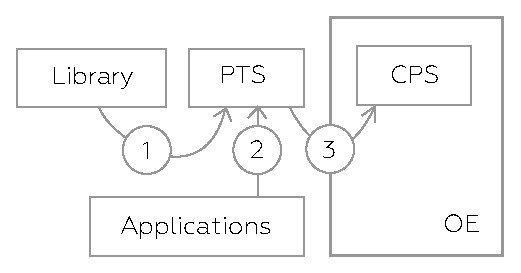
\includegraphics[scale=0.5]{minimal.eps}}
  \caption{Мінімальна система з чистої мови та інтерпретатора}
\end{figure}

\subsection{Максимальна система}
Інший приклад системи --- це максимальна система, яка містить усі формальні
мови програмування та формальне середовище виконання (порядок синтаксичних дерев
як параметрів при конструюванні мовної категорії може змінюватися, тут
генеалогія HTS не ведеться від MLTT, яке є розгалуженням).
\begin{equation}
Total = 
\begin{cases}
Ob: \{ O_{CPS}, O_{PTS}, O_{MLTT}, O_{ITS}, O_{HTS} \} \\
Hom: \begin{cases}
1,2: \mathbb{1} \rightarrow O_{HTS}, 3: O_{MLTT} \rightarrow O_{ITS} \\
4: O_{HTS} \rightarrow O_{ITS}, 5: O_{ITS} \rightarrow O_{PTS}, 6: O_{PTS} \rightarrow O_{CPS}
\end{cases}
\end{cases}
\end{equation}
За допомогою мереж Петрі це можна відобразити наступним чином:
\begin{figure}[h]
  \centerline{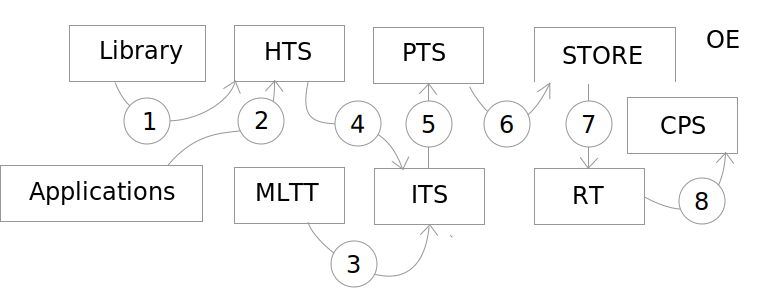
\includegraphics[scale=0.5]{full.eps}}
  \caption{Кубічна та чиста системи типів та середовище виконання}
\end{figure}

\newpage
\section{Формальні мови програмування}
Тут йдеться про мови програмування придатні для доведення теорем,
та їх таксономію від найелементарніших (чистої системи з одним типом $\Pi$) до
найпотужніших гомотопічних систем. Одна така гомотопічна система є кінцевим завданням
цього розділу --- побудова моделі гомотопічного верифікатора.
В процесі його побудови в цьому розділі ми розглянемо під
мікроскопом складові частини його нижчих мовних рівнів.

Застосуємо категорну семантику для мов програмування і будемо розглядати
мови програмування як моноїдальні мовні категорі, об'єкти яких є просторами
усіх програм цих мов програмування, а морфізми --- правила верифікації та компіляції цих мов.
Морфізми між мовними категоріями в категорї мов програмування --- це
функтори підвищення та пониження складності мови, подібно до того як діють
морфізми в контекстуальних категоріях. Морфізм деконструює або конструює за
допомогою Either-типу або $\Sigma$-типу індуктивний тип мови програмування.

Мови розкладаються у спектральну (індексовану натуральними числами $N \rightarrow U$)
послідовність мов, кожен елемент якої є мовою програмування,
яка не містить синтаксичне дерево вищої мови програмування.

\newpage
\subsection{Чиста система типів $O_{PTS}$}

Чиста ситема або числення конструкцій або система з одим типом або
система з однією аксіомою, продовжує традиції елементарних пруверів
в стилі першого AUTOMATH та сучасного Morte, Henk.

\begin{definition} (Мовна категорія чистої мови $O_{PTS}$).
\begin{equation}
O_{PTS} =
\begin{cases}
Ob: \{\ X: maybe\ PTS, target: maybe\ CPS \ \} \\
Hom: \begin{cases}
type,norm: X \rightarrow X, extract: X \rightarrow target \\
certify: X \rightarrow target = type \circ norm \circ extract
\end{cases}
\end{cases}
\end{equation}
\end{definition}

\begin{definition} (Синтаксис мовної категорії $O_{PTS}$).
Чиста мова $O_{PTS}$ містить лише синтаксис одного типу, $\Pi$-типу.
Така теорія називається теорією з одним типом, або з однією аксіомою.
\begin{lstlisting}
data PTS = ppure (_: pts PTS)
\end{lstlisting}
\end{definition}

Вона описана в літературі як Calculus of Construction (Кокан),
Pure Type System (Стемп, Фу).

\begin{definition} (Синтаксичне дерево $O_\Pi$).
\begin{lstlisting}[mathescape=true]
data pts (lang: U)
   = star (n: nat)
   | var (x: name) (l: nat)
   | pi (x: name) (l: nat) (f: lang)
   | lambda  (x: name) (l: nat) (f: lang)
   | app (f a: lang)
\end{lstlisting}
\end{definition}

\newpage
\subsection{Теорія типів Мартіна-Льофа $O_{MLTT}$}

Мова теорії типів є сучасною основою всіх пруверів з залежними типами,
такими, наприклад, як NuPRL та Agda. Багато так званих $\Pi\Sigma$ пруверів
імплементують $MLTT$ серед таких як:
$\Pi\Sigma$\footnote{\url{https://github.com/zlizta/pisigma-0-2-2}},
$\Pi\forall$\footnote{\url{https://github.com/sweirich/pi-forall}}.

\begin{definition} (Мовна категорія $O_{MLTT}$).
\begin{equation}
O_{MLTT} =
\begin{cases}
Ob: \{\ maybe\ MLTT\ \} \\
Hom: \begin{cases}
type,norm: Ob \rightarrow Ob \\
certify: Ob \rightarrow Ob = type \circ norm
\end{cases}
\end{cases}
\end{equation}
\end{definition}

\begin{definition} (Синтаксис мовної категорії $O_{MLTT}$).
Мова $O_{MLTT}$ включає в себе синтаксиси трьох типів
теорії Мартіна-Льофа: $O_\Pi$, $O_\Sigma$, $O_=$.
\begin{lstlisting}
data MLTT = mpure (_: pts MLTT)
          | msigma (_: exists MLTT)
          | mid (_: identity MLTT)
\end{lstlisting}
\end{definition}

\begin{definition} (Синтаксичне дерево $O_\Sigma$).
Також можна до чистої системи додати $\Sigma$-тип,
піднявши типову систему до мови $O_{MLTT-72}$ або $O_{\Pi\Sigma}$ :
\begin{lstlisting}[mathescape=true]
data exists (lang: U)
   = sigma (n: name) (a b: lang)
   | pair (a b: lang)
   | fst (p: lang)
   | snd (p: lang)
\end{lstlisting}
\end{definition}

\begin{definition} (Синтаксичне дерево $O_=$).
Додавши тип рівності можно підняти систему ще на одну сходинку,
до $O_{MLTT-84}$ або $O_{\Pi\Sigma=}$:
\begin{lstlisting}[mathescape=true]
data identity (lang: U)
   = id (t a b: lang)
   | id_intro (a b: lang)
   | id_elim (a b c d e: lang)
\end{lstlisting}
\end{definition}

\newpage
\subsection{Система індуктивних типів $O_{ITS}$}

\begin{definition} (Мовна категорія $O_{ITS}$).
\begin{equation}
O_{ITS} =
\begin{cases}
Ob: \{\ X: maybe\ ITS, target: maybe\ CPS\ \} \\
Hom: \begin{cases}
type,norm,induction: X \rightarrow X, extract: X \rightarrow target \\
certify : X \rightarrow target \\
cerfity = type \circ norm \circ induction \circ extract \\
\end{cases}
\end{cases}
\end{equation}
\end{definition}

Мова індуктивних типів дозволяє безпосередньо кодувати індуктивні типи,
не використовуючи схеми кодування Бома, містить усі попередні мовні синтаксиси:
$O_=$, $O_\Sigma$, $O_\Pi$.

\begin{definition} (Синтаксичне дерево мовної категорії $O_{ITS}$).
\begin{lstlisting}
data ITS = ipure (_: pts ITS)
         | isigma (_: exists ITS)
         | iid (_: identity ITS)
         | iITS (_: ind ITS)
\end{lstlisting}
\end{definition}

Мова містить наступні допоміжні визначення: i) телескопу,
який містить послідовність елементів мови; ii) розгалуження,
як конструкцій case оператора; iii) імен конструкторів індуктивного типу.

\begin{lstlisting}
data tele   (A: U) = emp | tel (n: name) (b: A) (t: tele A)
data branch (A: U) =        br (n: name) (args: list name) (term: A)
data label  (A: U) =       lab (n: name) (t: tele A)
                         | com (n: name) (t: tele A) (dim: list name)
                               (s: list  (prod (prod name bool) A))
\end{lstlisting}

\begin{definition} (Синтаксичне дерево $O_*$).
Правило формації, конструктора та елімінатора визначається синтаксичним деревом $O_*$:
\begin{lstlisting}
data ind (lang: U)
   = datum  (n: name) (t: tele lang) (labels:   list (label lang))
   | case   (n: name) (t: lang)      (branches: list (branch lang))
   | ctor   (n: name)                (args:     list lang)
\end{lstlisting}
\end{definition}

\newpage
\subsection{Гомотопічна система типів $O_{HTS}$}

\begin{definition} (Мовна категорія $O_{HTS}$).
$$
O_{HTS} =
\begin{cases}
Ob: \{\ maybe\ HTS\ \} \\
Hom: \begin{cases}
type,norm: Ob \rightarrow Ob \\
certify: Ob \rightarrow Ob = type \circ norm \\
\end{cases}
\end{cases}
$$
\end{definition}

\begin{definition} (Синтаксис мовної категорії $O_{HTS}$).
Синтаксис гомотопічної мовної категорії містить усі
попередні мовні синтаксиси: $O_I$, $O_W$, $O_=$, $O_\Sigma$, $O_\Pi$:
\begin{lstlisting}
data HTS = hpure (_: pts HTS)
         | hsigma (_: exists HTS)
         | hid (_: identity HTS)
         | hind (_: ind HTS)
         | homotopy (_: hts HTS)
\end{lstlisting}
\end{definition}

Гомотопічна типа наслідує $O_{ITS}$ але модифіковану з
Path-типом в індуктивних визначеннях, структурою композиції,
анонсує Path-тип (формація, конструктор, та елімінатор)
як лямбда функцію на відрізку, а також склейку типів у всесвіті
та склейку змінних з відповідними елімінаторами.

\begin{definition} (Синтаксичне дерево $O_I$).
\begin{lstlisting}
data hts (lang: U)
   = path (t a b: lang)
   | plam (n: name) (a: alg) (b: lang)
   | papp (f: name) (a: lang) (p: alg)
   | comp_ (a b: lang)
   | fill_ (a b c: lang)
   | glue_ (a b c: lang)
   | glue_elem (a b: lang)
   | unglue_elem (a b: lang)
\end{lstlisting}
\end{definition}

Таким чином,
$O_{HTS}$ містить два Id-типа, один унаслідований від $O_=$,
а інший який міститься в синтаксичному дереві $O_I$.

\newpage

\section{Формальне cередовище виконання}
Формальне середовище виконання складається з інтерпретатора
(нетитизованого $\lambda$-числення) та числення акторів (процесів, черг, таймерів).
Інтерпретатор та операційна система включені в систему доведення теорем
для уніфікації всіх сигнатур системи та формалізації самого інтерпретатора
як системи виконання. Слід зазначити, що не
завжди є змога зробити екстракт в $O_{CPS}$, тому об'єкти мовних
категорій є $maybe$-типами.
$$
O_{CPS}: O_\lambda \rightarrow O_\pi \rightarrow O_\mu \rightarrow U
$$
Далі буде йтися тільки про формальні інтерпретатори,
так як вони є найбільш компакними формами мов для
верифікації (в порівнянні з моделями System F).
Таким чином будемо розглядати формальне середовище виконання, як
сукупність інтерпретатора та операційної системи.

В цьому розділі ми побудуємо надшвидку імплементацію інтерпретатора,
яка цілком, разом зі своїми програмами, розміщується в кеш-памяті
першого рівня процесора, та здатна до AVX векторизацій засобами мови Rust.
Як промислова опція, підтримується також екстракт
в байт-код інтерпретатора BEAM віртуальної машини Erlang.


\newpage
\subsection{Категорія середовища виконання $O_{CPS}$}

\begin{definition} (Категорія середовища виконнання$O_{СPS}$).
$$
O_{CPS} =
\begin{cases}
Ob: \{\ maybe\ CPS\ \} \\
Hom: \{\ eval: Ob \rightarrow Ob\ \}
\end{cases}
$$
\end{definition}

Синтаксис середовища виконання може містити наступні синтаксиси:
$O_\lambda$, $O_\pi$, $O_\mu$.

\begin{definition} (Синтаксис мовної категорії $O_{HTS}$).
\begin{lstlisting}
data CPS = church (_: lambda CPS)
         | milner (_: pi     CPS)
         | tensor (_: mu     CPS)
\end{lstlisting}
\end{definition}

\begin{definition} (Синтаксичне дерево $O_\lambda$). Інтерпретатор визначається
своїм трьома конструкторами: номер змінної (індекс де Брейна),
лямбда функція та її апплікація:
\begin{lstlisting}
data lambda = var (x: nat)
            | lam (l: nat) (d: cps)
            | app (f a: cps)
\end{lstlisting}
Мовою інтерпретаторів є нетипизоване лямбда числення, однак в залежності
від складності інтерпретатора це дерево може виглядати по-різному.
\end{definition}

\begin{definition} (Синтаксичне дерево $O_\pi$).
Правило формації, конструктора та елімінатора визначається синтаксичним деревом $O_*$:
\begin{lstlisting}
data pi (lang: U)
   = process
   | spawn
   | snd
   | rcv
   | pub
   | sub
\end{lstlisting}
\end{definition}

Кожна секція цієї глави буде присвячена цим мовним компонентам
системи доведення теорем. В кінці розділу дається повна система, яка включає в себе усі
мови та усі мовні перетворення.



\newpage
\section{Чиста система типів PTS$^\infty$}

IEEE\footnote{IEEE Std 1012-2016  --- V\&V Software verification and validation} стандарт
та регуляторні документи ESA\footnote{ESA PSS-05-10 1-1 1995 -- Guide to software verification and validation}
визначають інтрументи та підходи до виробничого процесу верифікації та валідації.
Найбільш розвинені та потужні засоби вимагають застосування математичних мов та нотацій.
Ера верифікованої математики була започаткована верифікатором AUTOMATH\cite{deBruijn83} (де Брейн) розробленого
під керівництвом де Брейна, а також розвиток теорії типів Мартіна-Льофа\cite{Lof84}.
Сьогодні ми маємо Lean, Coq, F*, Agda мови які використовують числення
конструкцій, Calculus of Constructions\cite{Coq88} (CoC)
та числення індуктивних типів (Calculus of Inductive Constructions\cite{Pfenning89} (CiC).
Пізніше учень де Брейна, Хенк Барендрехт класифікував послаблені чисті
системи типів по трьом осям та візуазізував це за допомогою лямбда-куба\cite{Henk93}.
Чисті мови програмування вже були імплементовані раніше
(Morte\footnote{Gabriel Gonzalez. Haskell Morte Library} Габріеля Гонзалеза, Henk\cite{Erik97} Еріка Мейера).
Чисті системи типів це системи з однм $\Pi$-типом (або ще і $\Sigma$ як в ECC\cite{Ore92}, Оре),
з можливими розширеннями, такими як PTS$^\infty$ з бескінечною кількістю всесвітів\cite{Tonpa18} (Сохацький),
Cedil з self-типами\cite{Fu14}\cite{Stump17} (Стамп, Фу), система з К-правилами\cite{Barthe95} (Барте).

Головна мотивація чистих систем -- це простота аналізу ядра верифікатора,
можливість застосування сильної нормалізації та довірена зовнішня верифікація
та сертифікація завдяки простоті верифікатора (type checker), це означає, що
алгоритм верифікації повинен бути настільки простим, аби можна було
просто імплементувати його на будь-якій мові програмування. Приклади застовування
тут можуть бути: 1) формальна мова блокчейн контрактів (Pluto\footnote{Rebecca Valentine. Formal Specification of
the Plutus Core Language. 2017. \url{https://iohk.io/research/papers/#JT5XKNBP}});
2) сертифіковані обчислення для інтерпретаторів; 3) платіжні системи.

\subsection{Генерація сертифікованих програм}
Згідно ізоморфізму Каррі-Говарда-Ламбека або інтерпретації Брауера-Гейтінга-Колмогорова
існує взаємноознозначна відповідність між доведеннями теорем (або пруфтермами)
та лямбда функціями в теорії типів Мартіна-Льофа\cite{Lof84}.
Так як специфікація та доведення її відоповідності для певної програми
відбувається за допомогою мови з залежними типами, ми можемо екстрагувати
цільову імплементацію (зі стертою інформацією про типи) сертифікованої программи
в довільну мову програмування. У якості такої цільової мови підходять
майже усі інтерпретатор безтипового лямбда числення, такі як JavaScript,
Erlang, PyPy, LuaJIT, K.

Більш розвинені практики та підходи до кодогенерації та екстрагуванню
сертифікованих програм полягає у генерації С++ чи Rust програм, або програм
для нижчих систем лямюда-кубу, таких як System F або System F$_\omega$.
У цій роботі представлений екстракт в мову Erlang у якості цільового інтерпретатору.

\begin{table}[h]
\begin{center}
\caption{List of languages, tried as verification targets}
\label{tab:a}
\tabcolsep7pt\begin{tabular}{lcccc}
\hline
{\bf Target} & {\bf Class} & {\bf Intermediate} & {\bf Theory}\\
\hline
JVM        & interpreter/native   & Java       & F-sub\footnote{System F wit bounded quantification}\\
JVM        & interpreter/native   & Scala      & System F-omega\\
CLR        & interpreter/native   & F\#        & System F-omega\\
GHC        & compiler/native      & Haskell    & System D\\
GHC        & compiler/native      & Morte      & CoC\\
GHC,OCaml  & compiler/native      & Coq        & CiC\\
O,BEAM     & interpreter          & Om         & PTS$^\infty$ \\
JavaScript & interpreter/native   & PureScript & System F\\
\hline
\end{tabular}
\end{center}
\end{table}

{\bf PTS синтаксиси}. Мінімальне ядро з однією аксіомою
сприймає декілька лямбда ситаксисів.
Перший синтаксис сумісний з системою програмування
$morte$\footnote{http://github.com/Gabriel439/Haskell-Morte-Library}, та походить від неї.
Інший синтаксис сумісний з синтаксисом $cubical$\footnote{http://github.com/mortberg/cubicaltt}.
Планувалося також підтримати синтаксис $caramel$\footnote{https://github.com/MaiaVictor/caramel}.

$$
\begin{cases}
Sorts = U.\{i\},\ i : Nat\\
Axioms = U.\{i\} : U.\{inc\ i\}\\
Rules = U.\{i\} \leadsto U.\{j\} : U.\{max\ i\ j\}\\
\end{cases}
$$

Мова програмування Ом -- це мова з залежними типами, яка є розширенням
числення конструкцій (Calculus of Constructions, CoC) Тері Кокана. Саме з числення
конструкцій починається сучасна обчислювальна математика. В додаток до CoC,
наша мова Ом має предикативну ієрархію індексованих всесвітів. В цій мові немає
аксіоми рекурсії для безпосереднього визначення рекурсивних типів. Однак в цій мові
вцілому, рекурсивні дерева та корекурсія може бути визначена, або як кажуть, закодована.
Така система аксіом називається системою з однією аксіомою (або чистою системою), тому що в ній
існує тільки Пі-тип, а для кожного типу в теорії типів Мартіна Льофа існує п'ять
конструкцій: формація, інтро, елімінатор, бета та ета правила.

Усі терми підчиняються системі аксіом {\bf Axioms} всередині
послідовності всесвітів {\bf Sorts} та складність залежного
терму відповідає максимальній складності домена та кодомена
(правила {\bf Rules}). Таким чином визначається простір всесвітів,
та його конфігурація може бути записана згідно нотації
Барендрехта для систем з чистими типами:


\paragraph{}
Проміжна мова чистої системи типів Ом базується на мові
Henk\cite{Erik97}, вперше описаній Еріком Мейером та Саймоном Пейтоном Джонсом в 1997 році.
Пізніше Габріель Гонзалез імплементував на мові Haskell
верифікатор з посиланням на Henk, та використував кодування Бома для нерекурсивного
кодування рекурсивних індуктивних типів. Ця мова базується лише на $\Pi$-типі,
$\lambda$-функції, її елімінатора аплікації, $\beta$-редукції та $\eta$-експансії.
Дизайн мови Ом нагадує дизайн мов Henk та Morte.
Ця мова призначена бути максимально простою (повна імплементація займає 300 рядків),
формально верифікованою, здатною продукувати сертифіковані програми та
розповсюджувати їх за межі комп'ютера по мережах та недовірених каналах зв'язку,
та компілювати (верифікувати та екстрагувати) на цільових платформах за допомогою
тієї ж мови Ом, можливо імплементовоної на іншій мові програмування та вбудованої
в основну систему.

\newpage
\subsection{Синтаксис}

Синтаксис PTS сумісний з численням конструкцій (CoC) Тері Кокана,
та такими мовами як Morte та Henk.
Однак в системі PTS присутній індекс для всесвітів який
представлений натуральними числами. Тут наведений синтаксис у BNF нотації

\begin{lstlisting}[mathescape=true]
     I := #list #nat
     U := * + * . #nat
     O := U + I + ( O ) + O O + O $\rightarrow$ O
        + $\lambda$ ( I : O ) $\rightarrow$ O
        + $\forall$ ( I : O ) $\rightarrow$ O
\end{lstlisting}

Тут + --- сумма виразів, '.' --- конкатенація терміналів без пробілу,
:= --- оператор визначення BNF-правила, \#empty, \#nat, \#list --- вбудовані типи BNF-нотації
--- синтаксичні елементи BNF нотації,
а *,:, $\rightarrow$, (, ), $\lambda$, $\forall$ -- термінали або синтаксичні елементи мови програмування.
Еквівалентне визначення як ініціальний об'єкт категорій $O_{PTS}$ або $O_\Pi$
який може вмістити цей синтаксис містить всі правила виводу
внутрішньої мови категорії.

\begin{lstlisting}[mathescape=true]
data pts (lang: U)
   = star             (n: nat)
   | var    (x: name) (l: nat)
   | pi     (x: name) (l: nat) (d c: lang)
   | remote (n: name) (n: nat)
   | lambda (x: name) (l: nat) (d c: lang)
   | app                       (f a: lang)
\end{lstlisting}


\subsection{Всесвіти}

Мова PTS$^\infty$ -- це лямбда числення з залежними типами вищого порядку,
розширення числення конструкцій Кокана, або системи P$_\omega$ Барендрехта,
з предикативною (імпредикативною) ієрархією індексованих всесвітів.
Це розширення мотивоване консистентністю\cite{Lof75} в залежній теорії типів та
неможливістю кодування парадоксів Жирара-Хуркенса-Рассела\footnote{Так званий парадокс голяра який виникає в системах $U : U$}. Також для
забезпечення консистентності в мові PTS відсутня аксіома \lstinline{Fixpoint}, хоча
за допомогою рекурсивного трактування конструктора \lstinline{remote},
така можливість зберігається.

$$
    \mathrm{U_0} : \mathrm{U}_1 : \mathrm{U}_2 : \mathrm{U}_3 : ...
$$

Де $\mathrm{U_0}$ --- імпредикативний всесвіт,
   $\mathrm{U_1}$ --- перший предикативний всесвіт,
   $\mathrm{U_2}$ --- другий предикативний всесвіт,
   $\mathrm{U_3}$ --- третій предикативний всесвіт і т.д.

\begin{equation}
\tag{S}
\dfrac
{o : Nat}
{U_o}
\end{equation}

\newpage
\subsection*{Предикативні всесвіти}

Всі терми підпорядковуються системі аксіом А для послідовності всесвітів S.
Складність R залежності термів дорівнює максимальнії складної термів з
яких складаєтсья формула (або вираз мови). Система всесвітів описується
згідно SAR-нотації Барендрехта. Зауважте, що предикативні всесвіти
несумісні в Бом кодуванням, але ви можете переключати предикативність.

\[
\tag{$A_1$}
\dfrac{i: Nat, j: Nat, i < j}{U_i : U_j}
\]

\[
\tag{$R_1$}
\dfrac{i : Nat, j : Nat}{U_i \rightarrow U_j : U_{max(i,j)} }
\]

\subsection*{Імпредикативні всесвіти}
Стягуваний імпредикативний простір внизу ієрархії є єдиним можливим розширенням
предикативної ієрархії для того аби вона залишалась консистентною. Однак
в чистій системі типів PTS підтримується ієрархія бескінечних імпредикативних всесвітів.

\begin{equation}
\tag{$A_2$}
\dfrac
{i: Nat}
{U_i : U_{i+1}}
\end{equation}

\begin{equation}
\tag{$R_2$}
\dfrac
{i : Nat,\ \ \ \ j : Nat}
{U_i \rightarrow U_{j} : U_{j}}
\end{equation}

\subsection{Контексти}

Контексти моделюються словником з іменами змінних в верифікаторі.
Він може бути типизований як \lstinline{list Sigma}.
Правило елімінації тут не дається, після використання функції верифікації,
словник вивільняється з пам'яті.

\begin{equation}
\tag{Ctx-formation}
\dfrac
{}
{\Gamma : Ctx}
\end{equation}

\begin{equation}
\tag{Ctx-intro$_1$}
\dfrac
{\Gamma : Ctx}
{\emptyset : \Gamma}
\end{equation}

\begin{equation}
\tag{Ctx-intro$_2$}
\dfrac
{A : U_i,\ \ \ \ x : A,\ \ \ \ \Gamma : Ctx}
{(x : A)\ \vdash\ \Gamma : Ctx}
\end{equation}

\newpage
\subsection{Операційна семантика}

Операційна семантика --- це правила обчислення,
або $\beta$-,$\eta$-правила фьюжену інтро-правила та елімінаторів.
для визначення яких необхідно визначити:
1) інтро-правила, їх тип (правило формації), та класс (тип правила формації);
2) правило елімінації та залежної елімінації (індукції).
Таким чином будемо вважати, що операційна семантика системи типів $O_{PTS}$
буде складатися з 5 правил: формації, інтро-правило,
залежний елімінатор (індукція), $\beta$-редукція або правило обчислення,
$\eta$-експансія або правило унікальності.

\begin{equation}
\tag{$\Pi$-formation}
\dfrac
{A:U_i\ ,\ x:A \vdash B : U_j}
{\Pi\ (x:A) \rightarrow B : U_{p(i,j)}}
\end{equation}

\begin{equation}
\tag{$\lambda$-intro}
\dfrac
{x:A \vdash b : B}
{\lambda\ (x:A) \rightarrow b : \Pi\ (x: A) \rightarrow B }
\end{equation}

\begin{equation}
\tag{$App$-elimination}
\dfrac
{f: (\Pi\ (x:A) \rightarrow B)\ \ \ a: A}
{f\ a : B\ [a/x]}
\end{equation}

\begin{equation}
\tag{$\beta$-computation}
\dfrac
{x:A \vdash b: B\ \ \ a:A}
{(\lambda\ (x:A) \rightarrow b)\ a = b\ [a/x] : B\ [a/x]}
\end{equation}

\begin{equation}
\tag{subst}
\dfrac
{\pi_1 : A\ \ \ \ u:A \vdash \pi_2 : B}
{[\pi_1/u]\ \pi_2 : B}
\end{equation}

Перелік теорем (специфікації) для чистої системи типів можуть бути
прямо вбудовані в теорію типів, таким чином ми отримуємо логічний фреймворк
для перевірки імплементації залежної теорії.

\begin{lstlisting}[mathescape=true]
PTS (A: U): U
  = (Pi_Former: (A -> U) -> U)
  * (Pi_Intro: (B: A -> U) -> ((a: A) -> B a) -> (Pi A B))
  * (Pi_Elim: (B: A -> U) (a: A) -> (Pi A B) -> B a)
  * (Pi_Comp1: (B: A -> U) (a : A) (f: Pi A B) ->
    Equ (B a) (Pi_Elim B a (Pi_Intro B f)) (f a))
  * ((B: A -> U) (a: A) (f: Pi A B) ->
    Equ (Pi A B) f (\(x:A) -> f x))
\end{lstlisting}

Доведення цих теорем дано в модулі базової бібліотеки розділу 3.
Також можна повитися на інші доведення \cite{Henk93}.
Рівняння обсислювальної семантики (бета та ета правила) визначаються
за допомогою Path-типів, які визначаються $O_=$ або $O_I$ мовним синтаксисом.

Ці рівняння обчислювальної семантики представлені тут як Path-тип в вищій мові.
В чистій системі типів PTS з бескінечною кількістю всесвітів ми додається в AST
remote конструктор для завантаження файлів з локального довіреного сховища.
Рекурсія по цьому конструктору заборонена.

Індекси де брейна діють локально в межах одного імені.
При додаванні існуючого імені в контекст збільшується індекс цього імені.
Таким чином PTS верифікатор чистої системи типів відрізняється від
канонічного приклада алгоритма верифікації CoC\cite{Coq88}. Він включає
наступні функції мовної категорії: {\bf підстановка},
{\bf зсув імені}, {\bf нормалізація} термів, {\bf рівність}
за визначенням та {\bf верифікація}.

\subsection{Перевірка типів}

Для перевірки типів застосовується наступний алгоритм верифікації, який є основаю
усіх залежних систем. В чистих системах потрібно бути обережним з \lstinline{remote}
конструктором. Він використовуються для завантаження типів з локального довіреного сховища.
При дозволі рекурсії по \lstinline{remote} конструктору можливо реалізувати
self-типи\cite{Stump17}\cite{Fu14}.

\begin{lstlisting}[mathescape=true]
type (:star,N)     D $\rightarrow$ (:star,N+1)
     (:var,N,I)    D $\rightarrow$ :true = proplists:is_defined N B, om:keyget N D I
     (:remote,N)   D $\rightarrow$ om:cache (type N D)
     (:pi,N,0,I,O) D $\rightarrow$ (:star,h(star(type I D)),star(type O [(N,norm I)|D]))
     (:fn,N,0,I,O) D $\rightarrow$ let star (type I D), NI = norm I
                         in (:pi,N,0,NI,type(O,[(N,NI)|D]))
     (:app,F,A)    D $\rightarrow$ let T = type(F,D),
                            (:pi,N,0,I,O) = T, :true = eq I (type A D)
                         in norm (subst O N A)
\end{lstlisting}

\subsection{Індекси де Брейна}
Зсув переіменовує змінну N в контексті P, тобто додає одиницю для лічильника цієї змінної.

\begin{lstlisting}[mathescape=true]
  sh (:star,X)     N P $\rightarrow$ (:star,X)
     (:var,N,I)    N P $\rightarrow$ (:var,N,I+1) when I >= P
                       $\rightarrow$ (:var,N,I)
     (:remote,X)   N P $\rightarrow$ (:remote,X)
     (:pi,N,0,I,O) N P $\rightarrow$ (:pi,N,0,sh I N P,sh O N P+1)
     (:fn,N,0,I,O) N P $\rightarrow$ (:fn,N,0,sh I N P,sh O N P+1)
     (:app,L,R)    N P $\rightarrow$ (:app,L,R)
\end{lstlisting}

\subsection{Підстановка, нормалізація, рівність}
Підстановка заміняє змінну у виразі на певний терм.

\begin{lstlisting}[mathescape=true]
 sub (:star,X)     N V L $\rightarrow$ (:star,X)
     (:var,N,L)    N V L $\rightarrow$ V
     (:var,N,I)    N V L $\rightarrow$ (:var,N,I-1) when I > L
     (:remote,X)   N V L $\rightarrow$ (:remote,X)
     (:pi,N,0,I,O) N V L $\rightarrow$ (:pi,N,0,sub I N V L,sub O N (sh V N 0) L+1)
     (:pi,F,X,I,O) N V L $\rightarrow$ (:pi,F,X,sub I N V L,sub O N (sh V F 0) L)
     (:fn,N,0,I,O) N V L $\rightarrow$ (:fn,N,0,sub I N V L,sub O N (sh V N 0) L+1)
     (:fn,F,X,I,O) N V L $\rightarrow$ (:fn,F,X,sub I N V L,sub O N (sh V F 0) L)
     (:app,F,A)    N V L $\rightarrow$ (:app,   sub F N V L,sub A N V L)
\end{lstlisting}

Нормалізація виконує підстановку при аплікаціях до функцій (бета-редукція)
за допомогою рекурсивного спуску по конструкторам синтаксичного дерева.

\begin{lstlisting}[mathescape=true]
norm (:star,X)     $\rightarrow$ (:star,X)
     (:var,X)      $\rightarrow$ (:var,X)
     (:remote,N)   $\rightarrow$ cache (norm N [])
     (:pi,N,0,I,O) $\rightarrow$ (:pi,N,0,norm I,norm O)
     (:fn,N,0,I,O) $\rightarrow$ (:fn,N,0,norm I,norm O)
     (:app,F,A)    $\rightarrow$ case norm F of
                         (:fn,N,0,I,O) $\rightarrow$ norm (subst O N A)
                                    NF $\rightarrow$ (:app,NF,norm A) end
\end{lstlisting}

Рівність за визначенням перевіряє рівність Erlang термів.

\begin{lstlisting}[mathescape=true]
  eq (:star,N)        (:star,N)        $\rightarrow$ true
     (:var,N,I)       (:var,(N,I))     $\rightarrow$ true
     (:remote,N)      (:remote,N)      $\rightarrow$ true
     (:pi,N1,0,I1,O1) (:pi,N2,0,I2,O2) $\rightarrow$
          let :true = eq I1 I2
           in eq O1 (subst (shift O2 N1 0) N2 (:var,N1,0) 0)
     (:fn,N1,0,I1,O1) (:fn,N2,0,I2,O2) $\rightarrow$
          let :true = eq I1 I2
           in eq O1 (subst (shift O2 N1 0) N2 (:var,N1,0) 0)
     (:app,F1,A1)       (:app,F2,A2)   $\rightarrow$ let :true = eq F1 F2 in eq A1 A2
     (A,B)                             $\rightarrow$ (:error,(:eq,A,B))
\end{lstlisting}

\subsection{Використання мови}
Тут буде показано використання мови PTS.

\begin{lstlisting}
$ ./om help me
[{a,[expr],"to parse. Returns {_,_} or {error,_}."},
 {type,[term],"typechecks and returns type."},
 {erase,[term],"to untyped term. Returns {_,_}."},
 {norm,[term],"normalize term. Returns term's normal form."},
 {file,[name],"load file as binary."},
 {str,[binary],"lexical tokenizer."},
 {parse,[tokens],"parse given tokens into {_,_} term."},
 {fst,[{x,y}],"returns first element of a pair."},
 {snd,[{x,y}],"returns second element of a pair."},
 {debug,[bool],"enable/disable debug output."},
 {mode,[name],"select metaverse folder."},
 {modes,[],"list all metaverses."}]

$ ./om print fst erase norm a "#List/Cons"
   \ Head
-> \ Tail
-> \ Cons
-> \ Nil
-> Cons Head (Tail Cons Nil)
ok
\end{lstlisting}

\subsection{Екстракти}

Мова Ом передбачає автоматичну генерацію сертифікованих програм в цільові платформи.
Сертифікая полягаю у візуальному доведенню одніє стрілки ізоморфізма
$\lambda$-функції в залежній теорії типів та $\lambda$-фунції в нетипизованому лямбда численні.

\begin{lstlisting}[mathescape=true]
ext (:var,X,N,F)      $\rightarrow$ (:var,X)
    (:app,A,B,N,F)    $\rightarrow$ (:call,N,ext(F,A,N),[ext(F,B,N)])
    (:fn,S,_,I,O,N,F) $\rightarrow$ (:fun,N,(:clauses,[{:clause,N,
                                [(:var,N,S)],[],[ext(F,O,N)]}]))
                    _ $\rightarrow$ []
\end{lstlisting}

Так працьє функція екстракту в Erlang з системи типів PTS$^\infty$.
Erlang-версія Ом повинна бути зручна для використання для
віртуальних машин LING та BEAM. Оскільки цей екстракт генерує
AST дерево Erlang (подідбно до Elixir), результуючий код
подається повністью на весь стек оптимізаційного компілятора
Erlang включаючи Erlang Core, тому весь модуль екстракта займає 30 рядків.

\subsubsection{Інтерпретатори}
З практичною точки зору, мова Ом є способом використовувати залежні типи
та специфікації побудовані за їх допомогу на мові Erlang.
Завдяки глибокій інтеграції з Erlang вдалося мімізувати
імплементацію системи до 300 рядків.
Екстракт в інтерпретатор $O_{PTS}$ (чи інші) є альтернативною опцією для Ом.
Також мова Ом може бути легко портована на інші мови.

\subsubsection{LLVM}
Більш складна опція генерації сертифікованих програм --- це генерація машинного коду,
з використанням або без використання допоміжних проміжних мов таких як LLVM та MIR.
Тому що для цього потрібно верифікувати модель асемблера та процесора а також
його оптимізатора, так як зі складністю синтаксичного дерева росте складність
та велична терму-доведення будь-яких властивостей.

\subsubsection{FPGA}
Інша, не мен складна, або ще більш складна опція є безпосередня генерація
VHDL моделей (наприклад, clash).

\newpage
\section{Система індуктивних типів ITS}
Індуктивні синтаксиси та кодування можуть підтримуватися за допомогою системи модулів.
Кожна система модулів може самостійно (у вигляді ефектів), або за допомогою лямбда кодувань
попередньої мови PTS рівня, зберігати та оперувати індуктивними типами даних.

\subsection{Синтаксис}

\begin{lstlisting}[mathescape=true]
def := data id tele = sum + id tele : exp = exp +
       id tele : exp where def
exp := cotele*exp + cotele $\rightarrow$ exp + exp $\rightarrow$ exp + (exp) + app + id +
       (exp,exp) + \ cotele $\rightarrow$ exp + split cobrs + exp .1 + exp .2

  0 := #empty         imp    := [ import id ]
brs := 0 + cobrs      tele   := 0 + cotele
app := exp exp        cotele := ( exp : exp ) tele
 id := [ #nat ]       sum    := 0 + id tele + id tele | sum
ids := [ id ]         br     := ids $\rightarrow$ exp
cod := def dec        mod    := module id where imp def
dec := 0 + codec      cobrs  := | br brs
\end{lstlisting}

Індуктивні синтаксиси будуються на телескопах Диб'єра,
конструкторах сум, та їх елімінаторах.

\begin{lstlisting}
data tele   (A: U) = emp | tel (n: name) (b: A) (t: tele A)
data branch (A: U) =        br (n: name) (args: list name) (term: A)
data label  (A: U) =       lab (n: name) (t: tele A)
                         | com (n: name) (t: tele A) (dim: list name)
                               (s: list (prod (prod name bool) A))
\end{lstlisting}

\begin{lstlisting}
data ind (lang: U)
   = datum  (n: name) (t: tele lang) (labels:   list (label lang))
   | case   (n: name) (t: lang)      (branches: list (branch lang))
   | ctor   (n: name)                (args:     list lang)
\end{lstlisting}

\newpage
\subsection{Поліноміальні функтори}

\paragraph{}
Існує два види формальної рекурсії: 1) перша з найменшою нерухомою точкою
(як $F_A(X) = 1 + A \times X$ або $F_A(X) = A + X \times X$), іншими словами
рекурсія з базою (термінується $1$ або $A$). Списки та дерева є
прикладами таких рекурсивних структур з nil та leaf термінальними
конструкторами (або рекурсивні суми).
2) друга з найбільшою нерухомою точкою, або рекурсія без бази
(як $F_A(X) = A \times X$) --- така рекурсія не термінована на рівні типів,
та моделює нетерміновані послідовності, процеси тощо (або рекурсивні добутки).
Кодування найменшою нерухомою точкою ще називається кодуванням
добре-визначиними деревами або кодування поліноміальними функторами.

\paragraph{}
\noindent Натуральні числа: $\mu\ X \rightarrow 1 + X$\\
Списки елементів A: $\mu\ X \rightarrow 1 + A \times X$\\
Лямбда числення: $\mu\ X \rightarrow 1 + X \times X + X$\\
Потоки: $\nu\ X \rightarrow A \times X$\\
Потенційно нескінченний список елементів A: $\nu\ X \rightarrow 1 + A \times X$\\
Кінцеве дерево: $\mu\ X \rightarrow \mu\ Y \rightarrow 1 + X \times Y = \mu\ X = List\ X$\\

Для цих кодувань існує аналог кодування Чорча, який розповсюджує
кодування чистими функціями з нетипизованого лямбда числення до $\Pi$-типу.
Таке кодування називається кодуванням Бома-Беррардуччі, а просто кодування Бома.
Воно дозволяє кодувати індуктивні типи даних $\Pi$-типами чистими функціями.
Проте як було показано Жеверсом\cite{Geuvers01} неможливо побудувати принцип
індукції в чистих системх без використання в явному чи прихованому
вигляді \lstinline{Fixpoint} аксіоми. Також неможливо побудувати
J елімінатор Id типу закодованого в Бом кодуванні, а також
елімінатори гомотопічних примітивів, наприклад елімінатори гомотопічного
візрізка як \lstinline{funExt}, \lstinline{homotopy}.

\newpage
\subsection{Кодування Бома}
Тип даних List над даним типом А, може бути представлений як ініціальні алгебра
$(\mu L_A, in)$ функтору $L_A(X) = 1 + (A \times X)$. Позначається $\mu L_A = List(A)$.
Функції-конструктори $nil: 1 \rightarrow List(A)$ та
$cons: A \times List(A) \rightarrow List(A)$ визначені як
$nil = in \circ inl$ та $cons = in \circ inr$, таким чином $in = [nil,cons]$.
Для кожних двох функцій $c: 1 \rightarrow C$ та $h: A \times C \rightarrow C$,
катаморфізм $f = \llparenthesis [c,h] \rrparenthesis : List(A) \rightarrow C$
є унікальним розв'язком системи рівнянь:
$$
\begin{cases}
  f \circ nil  = c \\
  f \circ cons = h \circ (id \times f)
\end{cases}
$$
де $f = foldr(c,h)$. Маючи це, ініціальна алгебра представлена функтором
$\mu (1 + A \times X)$ та сумою морфізмів
$[1 \rightarrow List(A), A \times List(A) \rightarrow List(A)]$
як катаморфізму. Використовуючи це кодування, List-тип в базовій бібліотеці мови $O_{PTS}$
буде мати наступну форму:
$$
\begin{cases}
 foldr = \llparenthesis [ f \circ nil , h] \rrparenthesis, f \circ cons = h \circ (id \times f)\\
 len = \llparenthesis [ zero, \lambda\ a\ n \rightarrow succ\ n ] \rrparenthesis \\
 (++) = \lambda\ xs\ ys \rightarrow \llparenthesis [ \lambda (x) \rightarrow ys, cons ] \rrparenthesis (xs) \\
 map = \lambda\ f \rightarrow \llparenthesis [ nil, cons \circ (f \times id)] \rrparenthesis
\end{cases}
$$
\begin{lstlisting}[mathescape=true]
data list (A: U) = cons (x: A) (cs: list A) | nil
\end{lstlisting}
$$
\begin{cases}
list = \lambda\ ctor \rightarrow \lambda\ cons \rightarrow \lambda\ nil \rightarrow ctor\\
cons = \lambda\ x\ \rightarrow \lambda\ xs \rightarrow \lambda\ list \rightarrow \lambda\ cons \rightarrow\ \lambda\ nil \rightarrow cons\ x\ (xs\ list\ cons\ nil)\\
nil = \lambda\ list \rightarrow \lambda\ cons \rightarrow \lambda\ nil \rightarrow nil\\
\end{cases}
$$
\begin{lstlisting}[mathescape=true]
module list where
    map (A B: U) (f: A -> B) : list A -> list B
    length (A: U): list A -> nat
    append (A: U): list A -> list A -> list A
    foldl (A B: U) (f: B -> A -> B) (Z: B): list A -> B
    filter (A: U) (p: A -> bool) : list A -> list A
\end{lstlisting}
$$
\begin{cases}
len = foldr\ (\lambda\ x\ n \rightarrow succ\ n)\ 0\\
(++) = \lambda\ ys \rightarrow foldr\ cons\ ys\\
map = \lambda\ f \rightarrow foldr\ (\lambda x\ xs \rightarrow cons\ (f\ x)\ xs)\ nil\\
filter = \lambda\ p \rightarrow foldr\ (\lambda x\ xs \rightarrow if\ p\ x\ then\ cons\ x\ xs\ else\ xs)\ nil\\
foldl = \lambda\ f\ v\ xs = foldr\ (\lambda\ xg\rightarrow\ (\lambda \rightarrow g\ (f\ a\ x)))\ id\ xs\ v\\
\end{cases}
$$

\newpage
\section{Гомотопічна система типів HTS}

\subsection{Синтаксис}

\begin{lstlisting}[mathescape=true]
   sys := [ sides ]          side := (id=0)$\rightarrow$exp+(id=1)$\rightarrow$exp
  form := form\/f1+f1+f2    sides := #empty+cos+side
   cos := side,side+side,cos  mod := ${\bf module}$ id ${\bf where}$ imps dec
    f1 := f1/\f2               f2 := -f2+id+0+1
   imp := ${\bf import}$ id                 brs := #empty+cobrs
   app := exp exp             tel := #empty+cotel
  imps := #list imp         cotel := (exp:exp) tel
    id := #list #nat          dec := #empty+codec
    u2 := ${\bf glue}$+${\bf unglue}$+${\bf Glue}$                   u1 := ${\bf fill}$+${\bf comp}$
   ids := #list id             br := ids$\rightarrow$exp+ids@ids$\rightarrow$exp
 codec := def dec
 cobrs := | br brs
   sum := #empty+id tel+id tel|sum+id tel<ids>sys   
   def := ${\bf data}$ id tel=sum+id tel:exp=exp+id tel:exp ${\bf where}$ def
   exp := cotel*exp+cotel$\rightarrow$exp+exp$\rightarrow$exp+(exp)+id
          (exp,exp)+\cotele$\rightarrow$exp+${\bf split}$ cobrs+exp${\bf.1}$+exp${\bf.2}$+
          $\langle$ids$\rangle$exp+exp@form+app+u2 exp exp sys+u1 exp sys
\end{lstlisting}

Тут термінали := (визначенния), + (сума типів), \#empty (пустий тип), \#nat (тип натуральних чисел),
\#list (тип списків) --- є частинами BNF мови. Термінали
$\rvert$, :, *, $\langle$, $\rangle$, (, ), =, $\backslash$, /, -, $\rightarrow$, 0, 1, @, [, ],
$\mathbf{module}$, $\mathbf{import}$,
$\mathbf{data}$, $\mathbf{split}$, $\mathbf{where}$, $\mathbf{comp}$, $\mathbf{fill}$,
$\mathbf{Glue}$, $\mathbf{glue}$, $\mathbf{unglue}$,
$\mathbf{.1}$, $\mathbf{.2}$,
а також термінал $,$ є терміналами мови верифікатора гомотопічної системи типів.
Ця мова включає в себе: індуктивні типи, вищі індуктивні типи, оператори склеювання
для всесвітів та типів з відповідними елімінаторами. Усі ці концепції, та їх
моделі більш формально та детально описані у наступному розділі 3.

Система не повинна бути обмежена мовами та синтаксисами, ми покажемо як приклад,
підтримку гомотопічної мови з інтервалом [0,1] сумісної з $cubical$ та з пітримкою індуктивних
синтаксисів та кодувань попереднього рівня.

\begin{lstlisting}[mathescape=true]
data alg
   = zero
   | one
   | max (a b: alg)
   | min (a b: alg)

data hts
   = path (t a b: lang)
   | plam (n: name) (a: alg) (b: lang)
   | papp (f: name) (a: lang) (p: alg)
   | comp_ (a b: lang)
   | fill_ (a b c: lang)
   | glue_ (a b c: lang)
   | glue_elem (a b: lang)
   | unglue_elem (a b: lang)
\end{lstlisting}

\newpage
\section{Інтерпретатор та операційна система}

Мінімаль мова системи $O_{CPS}$ визначається простим
синтаксичним деревом

\begin{lstlisting}
data cps = var (x: nat)
         | lam (l: nat) (d: cps)
         | app (f a: cps)
\end{lstlisting}

Однак, на практиці, застосовують більш складні описи синтаксичних дерев,
зокрема для лінивих обчислень, та розширення синтаксичного дерева спеціальними
командами пов'язаними з середовищем виконання. Програми таких
інтерпретаторів відповідно виконуються у певній пам'яті, яка
використовується як контекст виконання. Кожна така програма крутиться
як одиниця виконання на певному ядрі процесора. Ситема процесів, де
кожен процес є CPS-програмою яку виконує інтерпретатор на певному ядрі.

Мотивація для побудови такого інтерпретатору, який повністю розміщується
разом зі программою в L1 стеку (який лімітований 64КБ) базується на успіху
таких віртуальних машин як LuaJIT, V8, HotSpot, а також векторних мов
програмування типу К та J. Якби ми могли побудувати дійсно швидкий інтерпретатор
який би виконував програми цілком в L1 кеші, байткод та стріми якого були би
вирівняні по словам архітектури, а для векторних обчислень застосовувалися би AVX інструкції,
які, як відомо перемагають по ціні-якості GPU обчислення. Таким чином, такий
інтерпретатор міг би, навіть без спеціалізованої JIT компіляції, скласти
конкуренцію сучасним промисловим інтерпретаторам, таким як Erlang, Python, K, LuaJIT.

Для дослідження цієї гіпотези мною було побудовано еспериментальний інтерпретатор
без байт-коду, але з вирівняним по словам архітерктури стріму команд, які є
безпосередньою машинною презентацією конструкторів індуктивних типів (enum) мови Rust.
Наступні результати були отримані після неотпимізованої версії інтерпретатора
пнри обчисленні факторіала (5) та функції Акермана у точці (3,4).

\begin{lstlisting}
Rust    0
Java    3
PyPy    8
O-CPS   291
Python  537
K       756
Erlang  10699/1806/436/9
LuaJIT  33856
\end{lstlisting}

\begin{lstlisting}
akkerman_k     635 ns/iter (+/- 73)
akkerman_rust  8,968 ns/iter (+/- 322)
\end{lstlisting}

Ключовим викликом тут стали лінійні типи мови Rust, які не дозволяють
звертатися до ссилок, які вже були оброблені, а це впливає на всю
архітектуру тензорного преставлення змінних в мові інтерпретатор $О_{CPS}$,
яка наслідує певним чином мову К.

\subsection{Векторизація засобами мови Rust}

\begin{lstlisting}
objdump ./target/release/o -d | grep mulpd
   223f1: c5 f5 59 0c d3    vmulpd (%rbx,%rdx,8),%ymm1,%ymm1
   223f6: c5 dd 59 64 d3 20 vmulpd 0x20(%rbx,%rdx,8),%ymm4,%ymm4
   22416: c5 f5 59 4c d3 40 vmulpd 0x40(%rbx,%rdx,8),%ymm1,%ymm1
   2241c: c5 dd 59 64 d3 60 vmulpd 0x60(%rbx,%rdx,8),%ymm4,%ymm4
   2264d: c5 f5 59 0c d3    vmulpd (%rbx,%rdx,8),%ymm1,%ymm1
   22652: c5 e5 59 5c d3 20 vmulpd 0x20(%rbx,%rdx,8),%ymm3,%ymm3
\end{lstlisting}

\subsection{Байт-код інтерпретатора}

Синтаксичне дерево, або неформалізований бай-код віртуальної
машини або інтерпретатора $O_{CPS}$ розкладається на два дерева, одне дерево
для управляючих команд інтерпретатора: Defer, Continuation, Start (початок програми),
Return (завершення програми).

\begin{lstlisting}
data Lazy = Defer (otree: NodeId) (a: AST) (cont: Cont)
          | Continuation (otree: NodeId) (a: AST) (cont: Cont)
          | Return (a: AST)
          | Start
\end{lstlisting}

Операції віртуальної машини: умовний оператор, оператор присвоєння, лямбда
функція та аплікація, є відображеннями на конструктори синтаксичного дерева.

\begin{lstlisting}
data Cont = Expressions (ast: AST) (vec: Option (Iter AST)) (cont: Cont)
          | Assign (ast: AST) (cont: Cont)
          | Cond (c,d: AST) (cont: Cont)
          | Func (a,b,c: AST) (cont: Cont)
          | List (acc: Vec AST) (vec: Iter AST) (i: Nat) (cont: Cont)
          | Call (a: AST) (i: Nat) (cont: Cont)
          | Return
          | Intercore (m: Message) (cont: Cont)
          | Yield (cont: Cont)
\end{lstlisting}

\newpage
\subsection{Синтаксис}

Синтаксис мови $O_{CPS}$ підтримує тензори, та звичайне лямбда числення
з значеннями у тензорах машинних типів даних: i32, i64.

\begin{lstlisting}[mathescape=true]
E: V | A | C
NC: ";" = [] | ";" m:NL = m
FC: ";" = [] | ";" m:FL = m
EC: ";" = [] | ";" m:EL = m
NL: NAME | o:NAME m:NC = Cons o m
FL: E | o:E | m:FC = Cons o m
EL: E | EC  | o:E m:EC = Cons o m
C: N | c:N a:C = Call c a
N: NAME | S | HEX | L | F
L: "(" ")" = [] | "([" c:NL "]" m:FL ")" = Table c m | "(" l:EL ")" = List l
F: "{" "}" = Lambda [] [] [] | "{[" c:NL "]" m:EL "}" = Lambda [] c m
                             | "{" m:EL "}" = Lambda [] [] m
\end{lstlisting}

Після парсера, синтаксичне дерево розкладається по наступним складовим: AST для
тензорів, визначення вищого рівня, Value для машинних слів, Scalar для
конструкцій мови, куд входить зокрема: списки та словники, умовний оператор,
присвоєння, визначення функції та її аплікація, UTF-8 літерал, та оператор
передачі управління в поток планувальника який закріплений за певним ядром CPU.

\begin{lstlisting}
data AST     = Atom (a: Scalar)
             | Vector (a: Vec AST)
\end{lstlisting}

\begin{lstlisting}
data Value   = Nil
             | SymbolInt (a: u16)
             | SequenceInt (a: u16)
             | Number (a: i64)
             | Float (a: f64)
             | VecNumber (Vec i64)
             | VecFloat (Vec f64)
\end{lstlisting}

\begin{lstlisting}
data Scalar  = Nil
             | Any
             | List (a: AST)
             | Dict (a: AST)
             | Call (a b: AST)
             | Assign (a b: AST)
             | Cond (a b c: AST)
             | Lambda (otree: Option NodeId) (a b: AST)
             | Yield (c: Context)
             | Value (v: Value)
             | Name (s: String)
\end{lstlisting}


\newpage
\subsection{Операційна система}
Перелічимо основні властивості операційної системи (прототип
якої опублікований на Github\footnote{\url{https://github.com/voxoz/kernel}}).

\subsection{Властивості}
Автобалансована низьколатентна, неблокована, без копіювання, система черг
з CAS-мультикурсорами, з пріоритетами задач та масштабованими таймерами.

\subsubsection{Асиметрична багапроцесорність}
Ядро системи використовує асиметричну багапроцесорність (АП)
для планування машинного часу. Так у системі для консольного
вводу-виводу та вебсокет моніторингу використовується окремий
ректор (закріплений за ядром процессора),
аби планування не впливало на програми на інших процесорах.
\paragraph{}
Це означає статичне закріплення певного атомарного процесу
обчислення за певним реактором, та навіть можливо дати гарантію, що
цей процес не перерветься при наступному кванті планування
ніяким іншим процесом на цьому ядрі (ситуація єдиного процесу
на реактор ядра процесору). Ядро системи постачається разом з конфігураційною
мовою для закріплення задач за реакторами:
\begin{lstlisting}
reactor[aux;0;mod[console;network]];
reactor[timercore;1;mod[timer]];
reactor[core1;2;mod[task]];
reactor[core2;3;mod[task]];
\end{lstlisting}

\subsubsection{Низьколатентність}
Усі реактори повинні намагатися обмежити IP-лічильник команд
діапазоном розміром з L1/L2 кеш об'єм процесора, для унеможливлення
колізій між ядрами на міжядерній шині можлива конфігурація, де
реактори виконують код, області пам'яті якого не перетинаються,
та обмежені об'ємом L1 кеш пам'яті що при наявній AVX векторизації
дать змогу повністю використовувати ресурси процесору наповну.

\newpage
\subsubsection{Мультикурсори}
Серцем низьколатентної системи транспорту є система наперед виділений
кільцевих буферів (які називаються секторами глобального кільця). У цій
системі кілець діє система курсорі для запису та читання, ці курсори
можуть мати різний напрямок руху.
\begin{figure}[h]
  \centerline{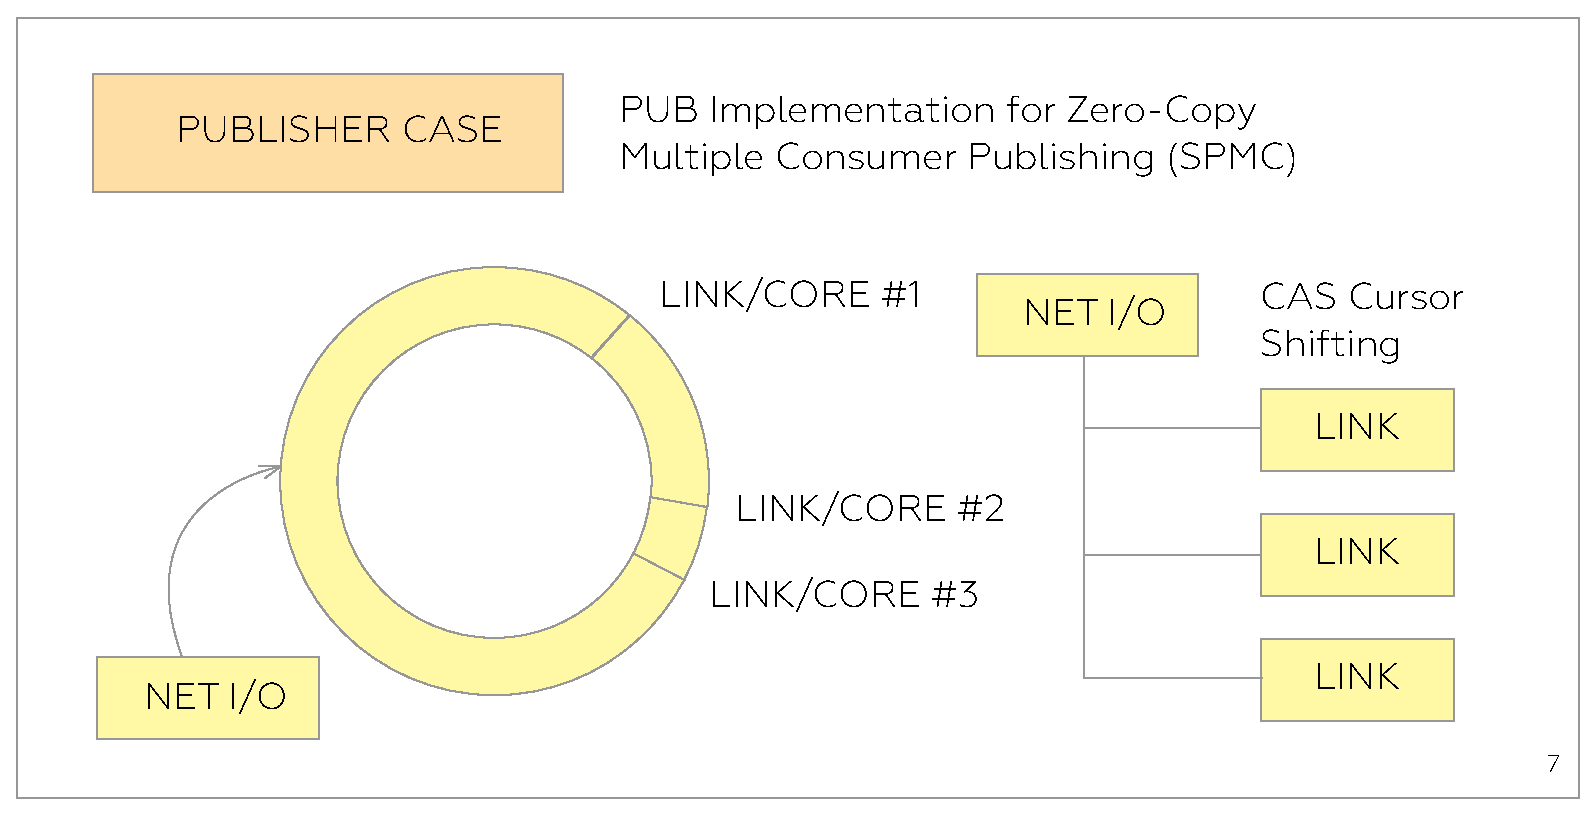
\includegraphics[scale=0.25]{pub.eps}}
  \caption{Кільцева статична черга з CAS-курсором для публікації}
\end{figure}
Для забезпечення імутабельності (нерухомості даних) та відсутності
копіювання в подальшій роботі, дані залишаються в черзі, а рухаються та передаються
лише курсори на типизовані послідовності даних.
\begin{figure}[h]
  \centerline{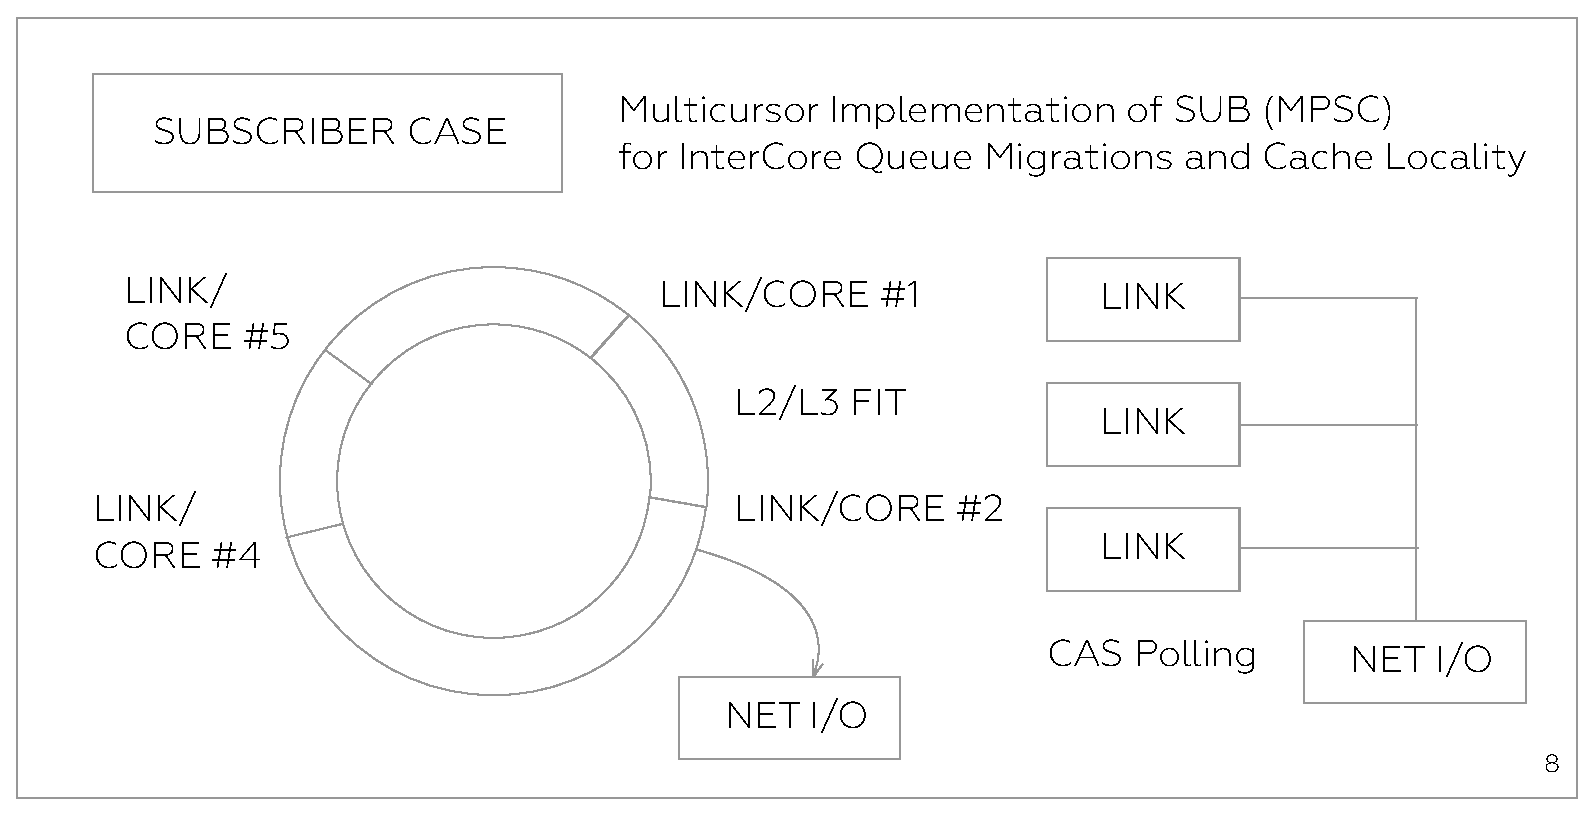
\includegraphics[scale=0.25]{sub.eps}}
  \caption{Кільцева статична черга з CAS-курсором для згортки}
\end{figure}

\newpage
\subsubsection{Реактори}
Кожен процесор має три типи реакторів які можуть бути на ньому запущені:
i) Task-реактор; ii) Timer-реактор; iii) IO-цикли. Для Task-реактора
існують черги пріорітетів, а для Timer-реактора --- дерева інтервалів.
\begin{figure}[h]
  \centerline{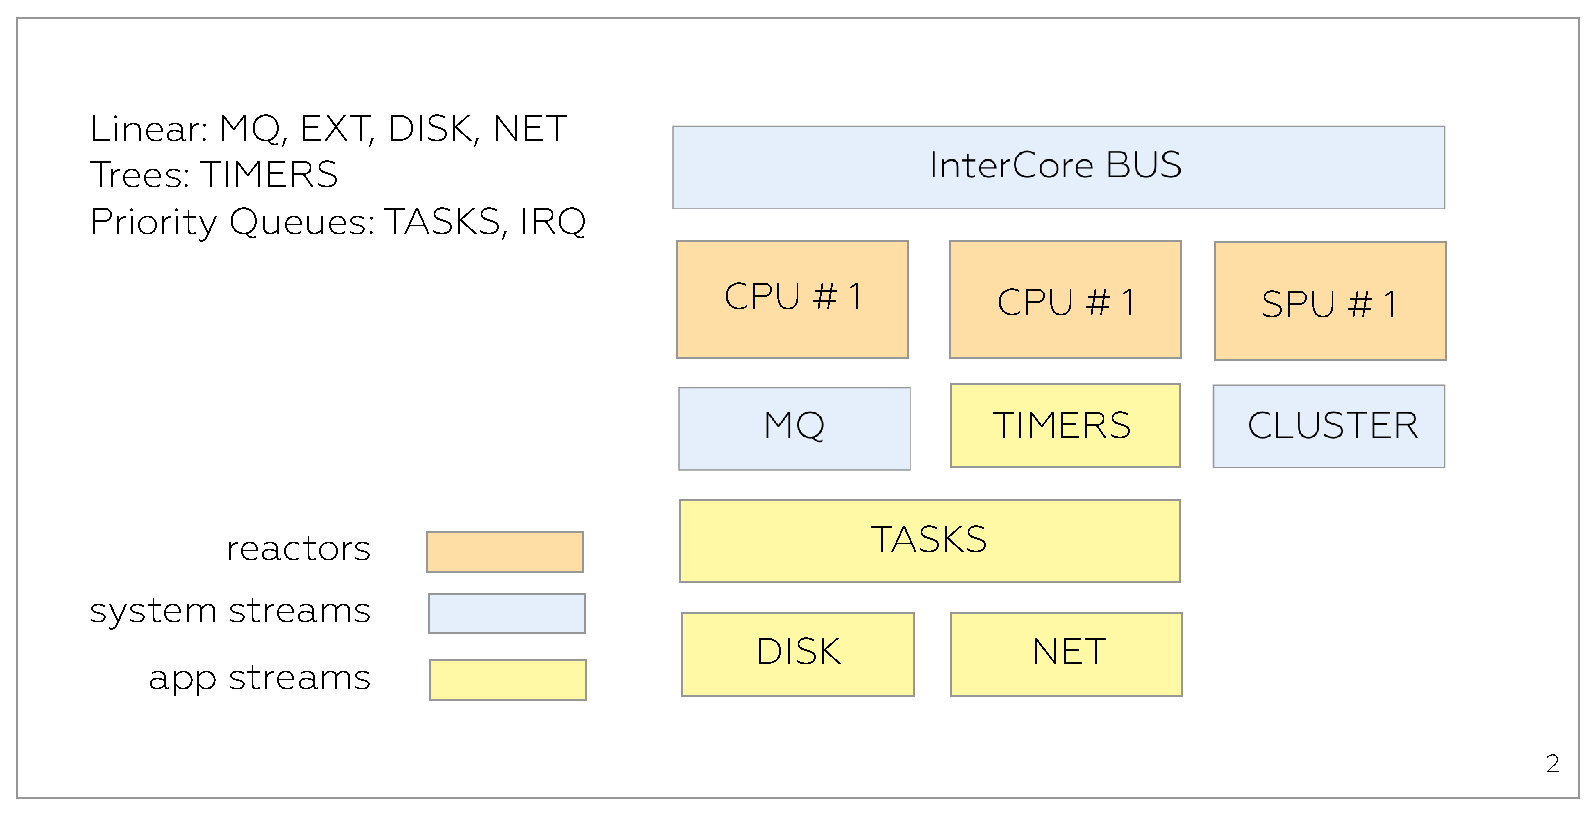
\includegraphics[scale=0.25]{sys.eps}}
  \caption{Система процесорних ядер та реакторів}
\end{figure}
Загальний спосіб комунікації для задач виглядає як публікація
в чергу (рух курсора запису) та підписка на черги і
згортання (руху курсора читання). Кожна черга має як
курсори для публікації так і курсори для читання. Можливо також
використання міжреакторної шини InterCore та посилання
службового повідомлення по цій шині на інший реактор. Так,
наприклад, працюють таймери та старти процесів, які передають
сигнал в реактор для перепланування. Можна створювати нові повідомлення
шини InterCore і систему фільтрів для згортання черги
реактора для більш гнучкої обробки сигналів реального часу.

\subsubsection*{Task-реактор}
Task-реактор або реактор задач виконує Rust задачі або
програми інтерпретатора, які можуть бути двох видів:
кінечні (які повертають результат виконання),
або бескінечні (процеси).
\begin{figure}[h]
  \centerline{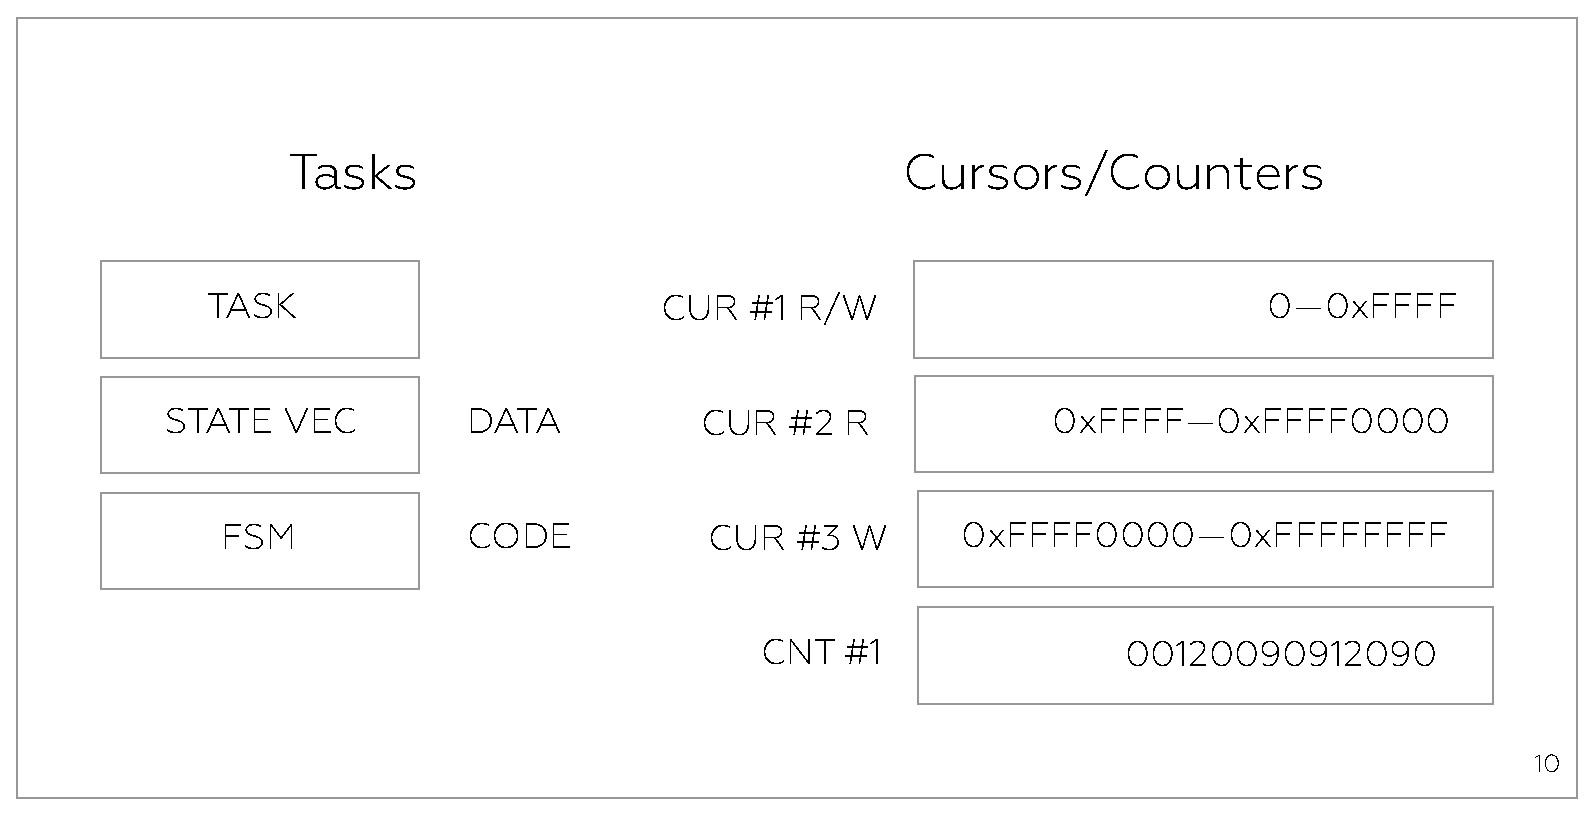
\includegraphics[scale=0.25]{task.eps}}
  \caption{Task-реактор або система інтерпретаторів}
\end{figure}

Приклад бескінечної задачі --- 0-процес,
який запускається при старті системи. Цей процес завжди доступний
по WebSocket каналу та з консолі терміналу.

\subsubsection*{IO-реактор}
Мережевий сервер або IO-реактор може обслуговувати багато
мережевих з'єднань та підтримує Windows, Linux, Mac смаки.
\begin{figure}[h]
  \centerline{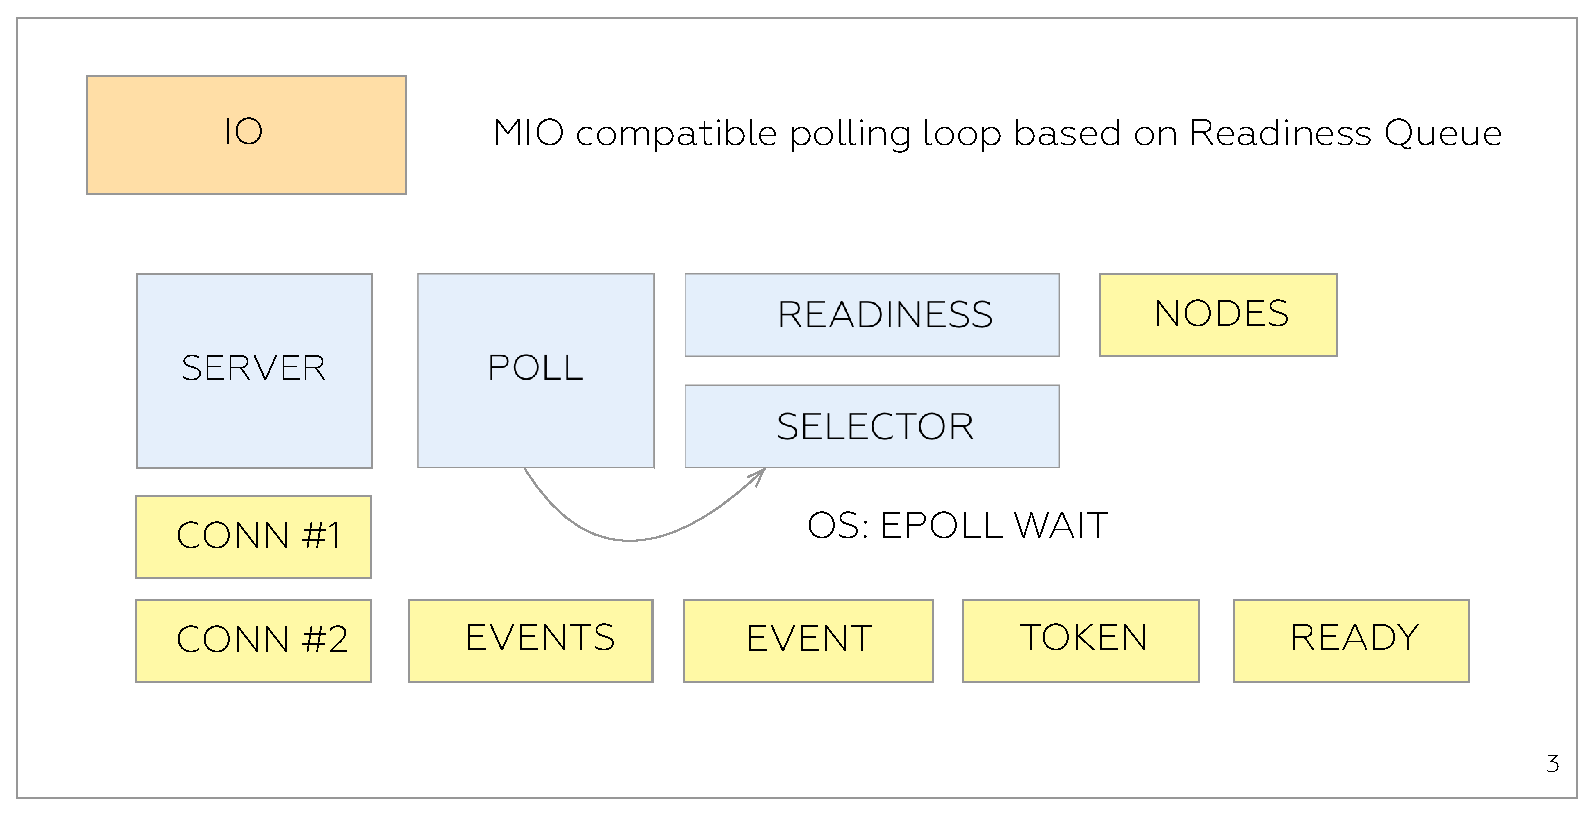
\includegraphics[scale=0.25]{net.eps}}
  \caption{IO-реактор або процес опитування мережевих сервісів}
\end{figure}

\subsubsection*{Timer-реактор}
Різні типи сутностей планування (такі як Task, IO, Timer)
мають різні дисципліни селекторів повідомлень для черг
(послідовно, через само-балансуючі дерева, BTree дерева тощо).
\begin{figure}[h]
  \centerline{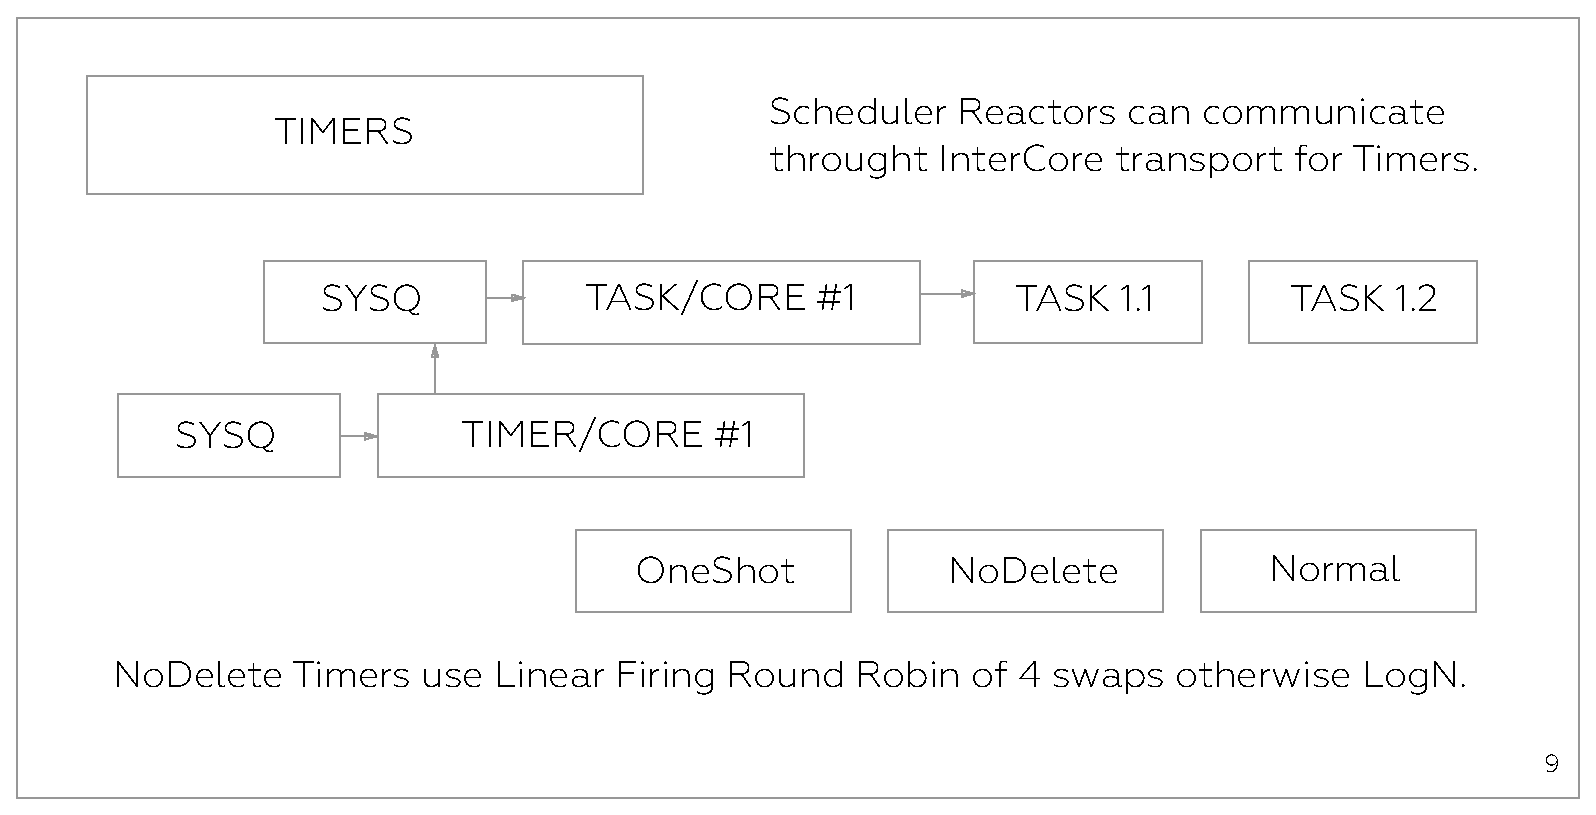
\includegraphics[scale=0.25]{timer.eps}}
  \caption{Timer-реактор або драйвер процесорного таймеру}
\end{figure}

\newpage
\subsubsection{Міжреакторний транспорт InterCore}
Шина InterCore конструюється певним числом SPMC черг, виділених для певного ядра.
Шина сама має топологію зірки між ядрами, та черга MPSC організована
як функція над множиною паблішерів. Кожне ядро має рівно одного паблішера.
Функція обробки шини протоколу InterCore називається poll\_bus та є членом планувальника.
Ви можете думати про InterCore як телепорт між процесорами, так як pull\_bus
викликається після кожної операції Yield в планувальник, і, таким чином,
якщо певному ядру опублікували в його чергу повідомлення, то після наступного Yield
на цьому ядрі буде виконана функція обробки цього повідомлення.

\subsubsection*{\lstinline{pub [ capacity ]}}
Створює новий CAS курсор для паблішінга, тобто для запису.
Повертає глобальних машинний ідентифікатор, має єдиний параметр, розмір черги.
Приклад: p: pub[16].

\subsubsection*{\lstinline{sub [ publisher ]}}
Створює новий CAS курсор для читання певної черги, певного врайтера.
Повертає глобальний машинний ідентифікатор для читання.
Приклад: s: sub[p].

\subsubsection*{\lstinline{spawn [ core ; program ; cursors ]}}
Створює нову програму задачу CPS-інтепреторатора для певного ядра.
Задача може бути або програмою на мові Rust або будь якою програмою через FFI.
Також при створенні задачі задається список курсорів,
які ексклюзивно належатимуть до цієї задачі.
Параметри функції: ядро, текст програми або назва FFI функції,спсисок курсорів.
Приклад: spawn[0;"etc/proc0";(0;1)].

\subsubsection*{\lstinline{snd [ writer ; data ]}}
Посилає певні дані в певний курсор для запису. Повертає Nil якшо всьо ОК.
Приклад: snd[p;42].

\subsubsection*{\lstinline{rcv [ reader ]}}
Повертає прочитані дані з певного курсору.
Якшо даних немає, то передає управління в планувальних за допомогою Yield.
Приклад: rcv[s].

\newpage
\subsection{Структури ядра}
Ядро є ситемою акторів з двома основними типами акторів:
чергами, які представляють кільцеві буфери та відрізки памяті;
та задачами, які резпрезентують байт-код програм та іх інтерпретацію на процесорі.
Черги бувають двох видів: для публікації, які місять курсори для запису;
та для читання, які містять курсори для читання. Задачі можна імплементувати
як Rust програми, або як $O_{CPS}$ програми.

\subsubsection{Черга для публікації}
\begin{lstlisting}
pub struct Publisher<T> {
    ring: Arc<RingBuffer<T>>,
    next: Cell<Sequence>,
    cursors: UncheckedUnsafeArc<Vec<Cursor>>,
}
\end{lstlisting}

\subsubsection{Черга для читання}
\begin{lstlisting}
pub struct Subscriber<T> {
    ring: Arc<RingBuffer<T>>,
    token: usize,
    next: Cell<Sequence>,
    cursors: UncheckedUnsafeArc<Vec<Cursor>>,
}
\end{lstlisting}

Існує дві спецільні задачі: InterCore задача, написана на Rust,
та запускається на всіх ядрах при запуску системи, а також CPS-інтерпретор
головного термінала системи, цей інтерпретор запускається на BSP ядрі,
поближче до Console та WebSocket IO селекторів.
В процесі життя різні CPS та Rust задачі можуть бути запущені в такій системі,
поєднуючи гнучкість програм інтерпретатора, та низькорівненивих програм написаних на мові Rust.

Окрім черг та задач, в системі присутні також таймери та інші IO задачі,
такі як сервери мережі або сервери доступу до файлів. Також існують
структури які репрезентують ядра та містять палнувальники.
Уся віртуальна машина є сукупністю таких структур-ядер.

\paragraph{}
\subsubsection{Канал}
Канал складається з одного курсору для запису та багатьох курсорів для читання.
Канал предствляє собою компонент зірки шини InterCore.
\begin{lstlisting}
pub struct Channel {
    publisher: Publisher<Message>,
    subscribers: Vec<Subscriber<Message>>,
}
\end{lstlisting}

\subsubsection{Черги ядра}
Память репрезентує усі наявні черги для публікації та читання на ядрі.
Ця інформація передається клонованою кожній задачі планувальника на цьому ядрі.
\begin{lstlisting}
pub struct Memory<'a> {
    publishers: Vec<Publisher<Value<'a>>,
    subscribers: Vec<Subscriber<Value<'a>>>,
}
\end{lstlisting}

\subsubsection{Планувальник}
Планувальник репрезентує ядро процесара,
які розрізняються як BSP-ядра (або 0-ядра, bootstrap)
та AP ядра (інші ядра > 0, application). BSP ядро
тримає на собі Console та WebSocket IO селектори.
Це означає, що BSP ядро дає свій час на обробку зовнішньої інформації,
у той час як AP процесори не обтяжені
таким навантаженням (io черга в таких планувальниках пуста).
Існує InterCore повідомлення яке додає або видаляє довільні IO селектори
в планувальних для довільних конфігурацій.

\begin{lstlisting}
pub struct Scheduler<'a> {
    pub tasks: Vec<T3<Job<'a>>>,
    pub bus: Channel,
    pub queues: Memory<'a>,
    pub io: IO,
}
\end{lstlisting}

\subsection{Протокол InterCore}

Протокол шини InterCore.

\begin{lstlisting}
pub enum Message {
    Pub(Pub),
    Sub(Sub),
    Print(String),
    Spawn(Spawn),
    AckSub(AckSub),
    AckPub(AckPub),
    AckSpawn(AckSpawn),
    Exec(usize, String),
    Select(String, u16),
    QoS(u8, u8, u8),
    Halt,
    Nop,
}
\end{lstlisting}

\newpage
\section{Висновки}

Як апогей, система HTS є фінальною категорією,
куди сходяться всі стрілки категорії мов. Кожна мова та її категорія
мають певний набір стрілок ендоморфізмів, які обчислюють, верифікують,
нормалізують, оптимізують програми своїх мов.
Стрілки виду $e_i: O_{n+1} \rightarrow O_n$ є екстракторами, які понижають систему типів,
при чому $O_{CPS} = O_0$.

Базова бібліотека мови Ерланг в яку проводиться основний
естракт йде з дистрибутивом Erlang/OTP. Базова бібліотека
$O_{PTS}$ наведена в репозиторії Github\footnote{\url{https://github.com/groupoid/om}}.
Гомотопічна базова бібліотека відповідає термінальній мові $O_{CCHM}$, та теж відкрита
на Github\footnote{\url{https://github.com/groupoid/infinity}}.
Останні два розділи присвячені математичному моделюванню математики на цій мові.

\subsection{Базова бібліотека}

Перша частина гомотопічної базової бібліотеки --- це основи гомотопічної теорії типів,
з основними визначеннями та теоремами.

\subsection{Математичні компоненти}

Друга частина гомотопічної базової бібліотеки --- це формалізація математики, як
приклад використання розробленої концепцтуальної моделі системи доведення теорем.


\addtocontents{toc}{\protect\newpage}
\chapter{ОСНОВА}

\section{Інтерналізація теорії типів}

Each language implementation needs to be checked. The one of possible test cases
for type checkers is the direct embedding of type theory model into the language of type checker.
As types in Martin-Löf Type Theory (MLTT) are formulated using 5 types of rules (formation,
introduction, elimination, computation, uniqueness), we construct aliases
for host language primitives and use type checker to prove that it is MLTT.
This could be seen as ultimate test sample for type checker as
intro-elimination fusion resides in beta-eta rules, so by proving them
we prove properties of the host type checker.

Also this issue opens a series of articles dedicated to formalization in
cubical type theory the foundations of mathematics. This issue is dedicated
to MLTT modeling and its verification. Also as many may not be familiar with
$\Pi$ and $\Sigma$ types, this issue presents different interpretation of MLTT types.

\subsubsection{Теорія типів}

MLTT could be reduced to $\Pi$, $\Sigma$, Path types, as W-types could be
modeled through $\Sigma$ and Fin/Nat/List/Maybe types could be modeled on W.
In this issue $\Pi$, $\Sigma$, Path are given as a core MLTT and W-types
are given as exercise. List, Nat, Fin types are defined in
next section.

Any new type in MLTT presented with set of 5 rules: i) formation rules, the signature of type;
ii) the set of constructors which produce the elements of formation rule signature;
iii) the dependent eliminator or induction principle for this type;
iv) the beta-equality or computational rule;
v) the eta-equality or uniquness principle. $\Pi$, $\Sigma$, and Path
types will be given shortly. This interpretation or rather way of modeling is MLTT specific.

The most interesting are Id types. Id types were added in \footnote{P. Martin-Löf, G. Sambin. Intuitionistic type theory. 1984.}{1984} while original MLTT was introduced in \footnote{P. Martin-Löf, G. Sambin. The Theory of Types. 1972.}{1972}.
Predicative Universe Hierarchy was added in \footnote{P. Martin-Löf. An intuitionistic theory of types: predicative part. 1975.}{1975}.
While original MLTT contains Id types that preserve uniquness of identity
proofs (UIP) or eta-rule of Id type, HoTT refutes UIP (eta rule desn't hold)
and introduces univalent heterogeneous Path equality (\footnote{M. Hofmann, T. Streicher. The groupoid interpretation of type theory. 1996.}{$\infty$-Groupoid interpretation}).
Path types are essential to prove computation and uniquness rules for all types
(needed for building signature and terms), so we will be able to prove all
the MLTT rules as a whole.

\subsubsection{Інтерпретації}

In contexts you can bind to variables (through de Brujin indexes or string names):
i) indexed universes; ii) built-in types; iii) user constructed types, and ask
questions about type derivability, type checking and code extraction. This system
defines the core type checker within its language.

\begin{table}
\centering
  \caption{Interpretations correspond to mathematical theories}\label{tab:pov}
 \begin{tabular}{lcccc}
    \hline
       Type Theory & Logic & Category Theory & Homotopy Theory\\
    \hline
       A type & class & object & space \\
       isProp A & proposition & (-1)-truncated object & space \\
       a:A program & proof & generalized element & point \\
       $B(x)$ & predicate & indexed object & fibration \\
       $b(x) : B(x)$ & conditional proof & indexed elements & section\\
       $\emptyset$ & $\bot$ false & terminal object & empty space \\
       $\mathbf{1}$ & $\top$ true & initial object & singleton \\
       $A + B$ & $A\vee B$ disjunction & coproduct & coproduct space \\
       $A\times B$ & $A\wedge B$ conjunction & product & product space \\
       $A\to B$ & $A\Rightarrow B$ & internal hom & function space \\
       $\sum{x:A},B(x)$ & $\exists_{x:A}B(x)$ & dependent sum & total space \\
       $\prod{x:A},B(x)$ & $\forall_{x:A}B(x)$ & dependent product & space of sections\\
       $\mathbf{Path}_{A}$ & equivalence $=_A$ & path space object & path space $A^I$ \\
       quotient & equivalence class & quotient & quotient \\
       W-type & induction & colimit & complex\\
       type of types & universe & object classifier & universe \\
       quantum circuit & proof net & string diagram & \\
      \hline
  \end{tabular}
\end{table}

By using this languages it is possible to encode different interpretations of
type theory itself and its syntax by construction. Usually the issues will refer to
following interpretations: i) type-theoretical; ii) categorical;
iii) set-theoretical; iv) homotopical; v) fibrational or geometrical.

\subsubsection*{Logical or Type-theoretical interpretation}

According to type theoretical interpretation for any type should be provided 5 formal
inference rules: i) formation; ii) introduction; iii) dependent elimination principle;
iv) beta rule or computational rule; v) eta rule or uniqueness rule. The last one could
be exceptional for Path types. The formal representation of all rules of MLTT
are given according to type-theoretical interpretation as a final result in this Issue I.
It was proven that classical Logic could be embedded into
intuitionistic propositional logic (IPL) which is directly embedded into MLTT.

Logical and type-theoretical interpretations could be distincted. Also
set-theoretical interpretation is not presented in Table 1.


\subsubsection*{Categorical or Topos-theoretical interpretation}

Categorical interpretation is a modeling through categories and functors.
First category is defined as objects, morphisms and their properties, then
we define functors, etc. In particular, as an example, according to categorical
interpretation $\Pi$ and $\Sigma$ types of MLTT are presented as adjoint
functors, and forms itself a locally closed cartesian category, which will be given a
intermediate result in {\bf Issue VII: Topos Theory}. In some sense we include here
topos-theoretical interpretations, with presheaf model of type theory as
example (in this case fibrations are constructes as functors, categorically).

\subsubsection*{Homotopical interpretation}

In classical MLTT uniquness rule of Id type do holds strictly. In Homotopical
interpretation of MLTT we need to allow a path space as Path type where uniqueness
rule doesn't hold. Groupoid interpretation of Path equality that doesn't hold UIP generally
was given in 1996 by Martin Hofmann and Thomas Streicher.

When objects are defined as fibrations, or dependent products, or indexed-objects
this leds to fibrational semantics and geometric sheaf interpretation. Several definition
of fiber bundles and trivial fiber bindle as direct isomorphisms of $\Pi$ types is
given here as theorem. As fibrations study in homotopical interpretation, geometric
interpretation could be treated as homotopical.

\subsubsection*{Set-theoretical interpretation}

Set-theoretical interpretations could replace first-order logic, but could not allow
higher equalities, as long as inductive types to be embedded directly. Set is modelled
in type theory according to homotopical interpretation as n-type.

\subsection{Типи $\Pi$, $\Sigma$, Path}

\subsubsection{$\Pi$-тип}

$\Pi$ is a dependent product type, the generalization of functions.
As a function it can serve the wide range of mathematical constructions as its domain and codomain,
which are in general: objects, types, or spaces; and could have as its
instance: sets, functions, polynomial functors, infinitesimals, $\infty$-groupoids,
topological $\infty$-groupoid, CW-complexes,
categories, languages, etc.

At this light there could be many interpretation of $\Pi$ types from different
areas of mathematics. We give here three: i) logical interpretation of $\Pi$ as
$\forall$ quantifier from higher order logic
that forms a ground of type theory; ii) geomeric intepretation of $\Pi$ as fiber bundle;
iii) categorical interpretation of functions as functors.

\subsubsection*{Теоретико-типова інтерпретація}

As a logical system dependent type theory could correspond to higher order logic.
However here only type-theoretical model is given completely.

\begin{definition} ($\Pi$-Formation).
$$(x: A) \rightarrow B(x) =_{def} \prod_{x:A}B(x) : U.$$
\begin{lstlisting}
Pi (A: U) (B: A -> U): U = (x: A) -> B x
\end{lstlisting}
\end{definition}

\begin{definition} ($\Pi$-Introduction).
$$\backslash (x: A) \rightarrow b =_{def} \prod_{A:U}\prod_{B:A \rightarrow U}\prod_{a: A}\prod_{b:B(a)}\lambda x.b : \prod_{y:A}B(a).$$
\begin{lstlisting}
lambda (A B: U) (b: B): A -> B = \ (x: A) -> b
lam (A:U) (B: A -> U) (a:A) (b:B a) : A -> B a = \ (x: A) -> b
\end{lstlisting}
\end{definition}

\begin{definition} ($\Pi$-Elimination).
$$f\ a =_{def} \prod_{A:U}\prod_{B: A \rightarrow U}\prod_{a:A}\prod_{f: \prod_{x:A}B(a)}f(a) : B(a).$$
\begin{lstlisting}
apply (A B: U) (f: A -> B) (a: A) : B = f a
app (A: U) (B: A -> U) (a: A) (f: A -> B a) : B a = f a
\end{lstlisting}
\end{definition}

\begin{theorem} ($\Pi$-Computation).
$$f(a) =_{B(a)} (\lambda (x:A) \rightarrow f(a))(a).$$
\begin{lstlisting}
Beta (A: U) (B: A -> U) (a: A) (f: A -> B a)
   : Path (B a) (app A B a (lam A B a (f a))) (f a)
\end{lstlisting}
\end{theorem}

\begin{theorem} ($\Pi$-Uniqueness).
$$f =_{(x:A)\rightarrow B(a)} (\lambda (y:A) \rightarrow f(y)).$$
\begin{lstlisting}
Eta (A: U) (B: A -> U) (a: A) (f: A -> B a)
  : Path (A -> B a) f (\(x:A) -> f x)
\end{lstlisting}
\end{theorem}

\subsubsection*{Категоріальна інтерпретація}

The adjoints $\Pi$ and $\Sigma$ is not the only adjoints could be presented in type system.
Axiomatic cohesions could contain a set of adjoint pairs as a core type checker operations.

\begin{definition} (Dependent Product).
The dependent product along morphism $g: B \rightarrow A$ in category $C$ is the right
adjoint $\Pi_g : C_{/B} \rightarrow C_{/A}$ of the base change functor.
\end{definition}

\begin{definition} (Space of Sections).
Let $\mathbf{H}$ be a $(\infty,1)$-topos, and let $E \rightarrow B : \mathbf{H}_{/B}$ a bundle in
$\mathbf{H}$, object in the slice topos. Then the space of sections $\Gamma_\Sigma(E)$
of this bundle is the Dependent Product:
$$ \Gamma_\Sigma(E) = \Pi_\Sigma (E) \in \mathbf{H}. $$
\end{definition}

\begin{theorem} (HomSet).
If codomain is set then space of sections is a set.
\begin{lstlisting}
setFun (A B : U) (_: isSet B) : isSet (A -> B)
\end{lstlisting}
\end{theorem}

\begin{theorem} (Contractability).
If domain and codomain is contractible then the space of sections is contractible.
\begin{lstlisting}
piIsContr (A: U) (B: A -> U) (u: isContr A)
          (q: (x: A) -> isContr (B x)) : isContr (Pi A B)
\end{lstlisting}
\end{theorem}

\begin{definition} (Section).
A section of morphism $f: A \rightarrow B$ in some category is the morphism $g: B \rightarrow A$
such that $f \circ g: B \mapright{g} A \mapright{f} B$ equals the identity morphism on B.
\end{definition}

\subsubsection*{Гомотопічна інтерпретація}

Geometrically, $\Pi$ type is a space of sections, while the dependent codomain is a space of fibrations.
Lambda functions are sections or points in these spaces, while the function result is a fibration.
$\Pi$ type also represents the cartesian family of sets, generalizing the cartesian product of sets.

\begin{definition} (Fiber).
The fiber of the map $p: E \rightarrow B$ in a point $y: B$ is all points $x: E$ such that $p(x)=y$.
\end{definition}

\begin{definition} (Fiber Bundle).
The fiber bundle $ F \rightarrow E \mapright{p} B$ on a total space $E$ with fiber layer $F$ and base $B$ is a
structure $(F,E,p,B)$ where $p: E \rightarrow B$ is a surjective map with following property:
for any point $y: B$ exists a neighborhood $U_b$ for which a homeomorphism $f: p^{-1}(U_b) \rightarrow U_b \times F$
making the following diagram commute.
\begin{center}
\begin{tikzpicture}
  \matrix (m) [matrix of math nodes,row sep=3em,column sep=3em,minimum width=2em]
  {
     {p^{-1}(U_b)} & {U_b \times F} \\
     U_b & \\};
  \path[-stealth]
    (m-1-1) edge node [above] {$f$}    (m-1-2)
            edge node [left]  {$p$}    (m-2-1)
    (m-1-2) edge node [right] {$pr_1$} (m-2-1);
\end{tikzpicture}
\end{center}
\end{definition}

\begin{definition} (Cartesian Product of Family over B).
Is a set $F$ of sections of the bundle with elimination map $app : F \times B \rightarrow E$ such that
\begin{equation}
F \times B \mapright{app} E \mapright{pr_1} B
\end{equation}
$pr_1$ is a product projection, so $pr_1$, $app$ are morphisms
of slice category $Set_{/B}$. The universal mapping property of $F$:
for all $A$ and morphism $A \times B \rightarrow E$ in $Set_{/B}$ exists
unique map $A \rightarrow F$ such that everything commute. So a category
with all dependent products is necessarily a category with all pullbacks.
\end{definition}

\begin{definition} (Trivial Fiber Bundle).
When total space $E$ is cartesian product $\Sigma(B,F)$ and $p = pr_1$
then such bundle is called trivial $(F,\Sigma(B,F),pr_1,B)$.
\end{definition}

\begin{theorem} (Functions Preserve Paths).
For a function $f: (x:A) \rightarrow B(x)$
there is an $ap_f : x =_A y \rightarrow f(x) =_{B(x)} f(y)$. This is called
application of $f$ to path or congruence property (for non-dependent case ---
$cong$ function). This property behaves functoriality
as if paths are groupoid morphisms and types are objects.
\end{theorem}

\begin{theorem} (Trivial Fiber equals Family of Sets).
Inverse image (fiber) of fiber bundle $(F,B*F,pr_1,B)$ in point $y:B$ equals $F(y)$.
\begin{lstlisting}
FiberPi (B: U) (F: B -> U) (y: B)
      : Path U (fiber (Sigma B F) B (pi1 B F) y) (F y)
\end{lstlisting}
\end{theorem}

\begin{theorem} (Homotopy Equivalence).
If fiber space is set for all base, and
there are two functions $f,g : (x:A) \rightarrow B(x)$ and two
homotopies between them, then these homotopies are equal.
\begin{lstlisting}
setPi (A: U) (B: A -> U) (h: (x: A) -> isSet (B x)) (f g: Pi A B)
      (p q: Path (Pi A B) f g) : Path (Path (Pi A B) f g) p q
\end{lstlisting}
\end{theorem}

Note that we will not be able to prove this theorem
until {\bf Issue III: Homotopy Type Theory} because
bi-invertible iso type will be announced there.

\subsubsection{$\Sigma$-тип}

$\Sigma$ is a dependent sum type, the generalization of products.
$\Sigma$ type is a total space of fibration. Element of total
space is formed as a pair of basepoint and fibration.

\subsubsection{Теоретико-типов інтерпретація}

\begin{definition} ($\Sigma$-Formation).
\begin{lstlisting}
Sigma (A : U) (B : A -> U) : U = (x : A) * B x
\end{lstlisting}
\end{definition}

\begin{definition} ($\Sigma$-Introduction).
\begin{lstlisting}
dpair (A: U) (B: A -> U) (a: A) (b: B a) : Sigma A B = (a,b)
\end{lstlisting}
\end{definition}

\begin{definition} ($\Sigma$-Elimination).
\begin{lstlisting}
pr1 (A: U) (B: A -> U)
    (x: Sigma A B): A = x.1

pr2 (A: U) (B: A -> U)
    (x: Sigma A B): B (pr1 A B x) = x.2

sigInd (A: U) (B: A -> U) (C: Sigma A B -> U)
       (g: (a: A) (b: B a) -> C (a, b))
       (p: Sigma A B) : C p = g p.1 p.2
\end{lstlisting}
\end{definition}

\begin{theorem} ($\Sigma$-Computation).
\begin{lstlisting}
Beta1 (A: U) (B: A -> U)
      (a:A) (b: B a)
    : Equ A a (pr1 A B (a,b))

Beta2 (A: U) (B: A -> U)
      (a: A) (b: B a)
    : Equ (B a) b (pr2 A B (a,b))
\end{lstlisting}
\end{theorem}

\begin{theorem} ($\Sigma$-Uniqueness).
\begin{lstlisting}
Eta2 (A: U) (B: A -> U) (p: Sigma A B)
   : Equ (Sigma A B) p (pr1 A B p,pr2 A B p)
\end{lstlisting}
\end{theorem}

\subsubsection{Категоріальна інтерпретація}

\begin{definition} (Dependent Sum).
The dependent sum along the morphism $f: A \rightarrow B$ in category $C$ is the left
adjoint $\Sigma_f : C_{/A} \rightarrow C_{/B}$ of the base change functor.
\end{definition}

\subsubsection{Теоретико-типова інтерпретація}

\begin{theorem} (Axiom of Choice).
If for all $x : A$ there is $y : B$ such that $R(x,y)$,
then there is a function $f : A \rightarrow B$
such that for all $x : A$ there is a witness of $R(x,f(x))$.
\begin{lstlisting}
ac (A B: U) (R: A -> B -> U)
 : (p: (x:A) -> (y:B)*(R x y)) -> (f:A->B) * ((x:A)->R(x)(f x))
\end{lstlisting}
\end{theorem}

\begin{theorem} (Total).
If fiber over base implies another fiber
over the same base then we can construct total space of section
over that base with another fiber.
\begin{lstlisting}
total (A:U) (B C: A -> U)
      (f: (x:A) -> B x -> C x) (w: Sigma A B)
    : Sigma A C = (w.1,f (w.1) (w.2))
\end{lstlisting}
\end{theorem}

\begin{theorem} ($\Sigma$-Contractability). If the fiber is set then the $\Sigma$ is set.
\begin{lstlisting}
setSig (A:U) (B: A -> U) (sA: isSet A)
       (sB : (x:A) -> isSet (B x)) : isSet (Sigma A B)
\end{lstlisting}
\end{theorem}

\begin{theorem} (Path Between Sigmas).
Path between two sigmas $t,u: \Sigma(A,B)$ could be decomposed to
sigma of two paths $p:t_1=_{A}u_1)$ and $(t_2=_{B(p@i)}u_2)$.
\begin{lstlisting}
pathSig (A:U) (B : A -> U) (t u : Sigma A B)
      : Path U (Path (Sigma A B) t u)
               ((p: Path A t.1 u.1) * PathP (<i>B(p@i)) t.2 u.2)
\end{lstlisting}
\end{theorem}

\subsubsection{Path-тип}

The Path identity type defines a Path space with elements and values.
Elements of that space are functions from interval $[0,1]$ to a values of that path space.
This ctt file reflects \footnote{Cyril Cohen, Thierry Coquand, Simon Huber, Anders M{\"{o}}rtberg. Cubical Type Theory: a constructive interpretation of the univalence axiom. 2015. \url{https://5ht.co/cubicaltt.pdf}}{CCHM} cubicaltt model with connections.
For \footnote{Carlo Angiuli, Brunerie, Coquand, Kuen-Bang Hou (Favonia), Robert Harper, Dan Licata. Cartesian Cubical Type Theory. 2017. \url{https://5ht.co/cctt.pdf}}{ABCFHL} yacctt model with
variables please refer to ytt file. You may also want to
read \footnote{Marc Bezem, Thierry Coquand, Simon Huber. A model of type theory in cubical sets. 2014. \url{http://www.cse.chalmers.se/~coquand/mod1.pdf}}{BCH},
\footnote{Carlo Angiuli, Kuen-Bang Hou (Favonia), Robert Harper. Cartesian Cubical Computational Type Theory: Constructive Reasoning with Paths and Equalities. 2018. \\ \url{https://www.cs.cmu.edu/~cangiuli/papers/ccctt.pdf}}{AFH}.
There is a \footnote{Andrew Pitts, Ian Orton. Axioms for Modelling Cubical Type Theory in a Topos. 2016. \url{https://arxiv.org/pdf/1712.04864.pdf}}{PO} paper about CCHM axiomatic in a topos.

\subsubsection{Кубічна інтерпретація}

\begin{definition} (Path Formation).
\begin{lstlisting}
Hetero (A B: U) (a: A) (b: B) (P: Path U A B) : U = PathP P a b
Path (A: U) (a b: A) : U = PathP (<i> A) a b
\end{lstlisting}
\end{definition}

\begin{definition} (Path Reflexivity).
Returns an element of reflexivity path space for a given value of the type.
The inhabitant of that path space is the lambda on the homotopy
interval $[0,1]$ that returns a constant value a. Written in
syntax as |<i>a| which equals to $\lambda\ (i: I) \rightarrow a$.
\begin{lstlisting}
refl (A: U) (a: A) : Path A a a
\end{lstlisting}
\end{definition}

\begin{definition} (Path Application).
You can apply face to path.
\begin{lstlisting}
app1 (A: U) (a b: A) (p: Path A a b): A = p @ 0
app2 (A: U) (a b: A) (p: Path A a b): A = p @ 1
\end{lstlisting}
\end{definition}

\begin{definition} (Path Composition).
Composition operation allows to build a new path by given to paths
in a connected point.
\begin{center}
\begin{tikzpicture}
  \matrix (m) [matrix of math nodes,row sep=3em,column sep=3em,minimum width=3em]
  {
     a & c \\ % (1,1) (1,2)
     a & b \\ % (2,1) (2,2)
  };
  \path[-stealth]
    (m-1-1) edge node [above] {$comp$} (m-1-2)
    (m-2-1) edge node [left]  {$\lambda(i:I)\rightarrow a$} (m-1-1)
    (m-2-2) edge node [right] {$q$} (m-1-2)
    (m-2-1) edge node [above] {$p @ i$} (m-2-2);
\end{tikzpicture}
\end{center}
\begin{lstlisting}
composition (A: U) (a b c: A) (p: Path A a b) (q: Path A b c)
          : Path A a c = comp (<i>Path A a (q@i)) p []
\end{lstlisting}
\end{definition}

\begin{theorem} (Path Inversion).
\begin{lstlisting}
inv (A: U) (a b: A) (p: Path A a b): Path A b a = <i> p @ -i
\end{lstlisting}
\end{theorem}

\begin{definition} (Connections).
Connections allows you to build square
with given only one element of path: i) $\lambda\ (i,j: I) \rightarrow p\ @\ min(i,j)$;
ii) $\lambda\ (i,j:I) \rightarrow p\ @\ max(i,j)$.
\begin{center}
  \begin{tikzpicture}
  \matrix (m) [matrix of math nodes,row sep=3em,column sep=3em,minimum width=3em]
  {
     a & b \\ % (1,1) (1,2)
     a & a                    \\ % (2,1) (2,2)
  };
  \path[-stealth]
    (m-1-1) edge node [above] {$p$}    (m-1-2)
    (m-2-1) edge node [left]  {$\lambda\ (i:I)\rightarrow a$}    (m-1-1)
    (m-2-2) edge node [right] {$p$} (m-1-2)
    (m-2-1) edge node [above] {$\lambda\ (i:I)\rightarrow a$} (m-2-2);
  \end{tikzpicture}
  \begin{tikzpicture}
  \matrix (m) [matrix of math nodes,row sep=3em,column sep=3em,minimum width=3em]
  {
     b & b \\ % (1,1) (1,2)
     a & b                    \\ % (2,1) (2,2)
  };
  \path[-stealth]
    (m-1-1) edge node [above] {$\lambda\ (i:I) \rightarrow b$}    (m-1-2)
    (m-2-1) edge node [left]  {$p$}    (m-1-1)
    (m-2-2) edge node [right] {$\lambda\ (i:I) \rightarrow b$} (m-1-2)
    (m-2-1) edge node [above] {$p$} (m-2-2);
  \end{tikzpicture}
\end{center}
\begin{lstlisting}
connection1 (A: U) (a b: A) (p: Path A a b)
          : PathP (<x> Path A (p@x) b) p (<i>b)
          = <y x> p @ (x \/ y)

connection2 (A: U) (a b: A) (p: Path A a b)
          : PathP (<x> Path A a (p@x)) (<i>a) p
          = <x y> p @ (x /\ y)
\end{lstlisting}
\end{definition}

\begin{theorem} (Congruence).
Is a map between values of one type
to path space of another type by an encode function between types.
Implemented as lambda defined on $[0,1]$ that returns
application of encode function to path application of
the given path to lamda argument |$\lambda$ (i:I) $\rightarrow$ f (p @ i)|
for both cases.
\begin{lstlisting}
ap  (A B: U) (f: A -> B)
    (a b: A) (p: Path A a b)
  : Path B (f a) (f b)

apd (A: U) (a x:A) (B: A -> U) (f: A -> B a)
    (b: B a) (p: Path A a x)
  : Path (B a) (f a) (f x)
\end{lstlisting}
\end{theorem}

\begin{theorem} (Transport).
Transports a value of the domain type to the value of the codomain type
by a given path element of the path space between domain and codomain types.
Defined as path composition with |[]| of a over a path $p$ --- |comp p a []|.
\begin{lstlisting}
trans (A B: U) (p: Path U A B) (a: A) : B
\end{lstlisting}
\end{theorem}

\subsubsection{Теоретико-типова інтерпретація}

\begin{definition} (Singleton).
\begin{lstlisting}
singl (A: U) (a: A): U = (x: A) * Path A a x
\end{lstlisting}
\end{definition}

\begin{theorem} (Singleton Instance).
\begin{lstlisting}
eta (A: U) (a: A): singl A a = (a,refl A a)
\end{lstlisting}
\end{theorem}

\begin{theorem} (Singleton Contractability).
\begin{lstlisting}
contr (A: U) (a b: A) (p: Path A a b)
  : Path (singl A a) (eta A a) (b,p)
  = <i> (p @ i,<j> p @ i/\j)
\end{lstlisting}
\end{theorem}

\begin{theorem} (Path Elimination, Diagonal).
\begin{lstlisting}
D (A: U) : U = (x y: A) -> Path A x y -> U
J (A: U) (x y: A) (C: D A)
  (d: C x x (refl A x))
  (p: Path A x y) : C x y p
= subst (singl A x) T (eta A x) (y, p) (contr A x y p) d where
  T (z: singl A x) : U = C x (z.1) (z.2)
\end{lstlisting}
\end{theorem}

\begin{theorem} (Path Elimination, Paulin-Mohring).
J is formulated in a form of Paulin-Mohring and implemented using
two facts that singleton are contractible and dependent function
transport.
\begin{lstlisting}
J (A: U) (a b: A)
  (P: singl A a -> U)
  (u: P (a,refl A a))
  (p: Path A a b) : P (b,p)
\end{lstlisting}
\end{theorem}

\begin{theorem} (Path Elimination, HoTT).
J from HoTT book.
\begin{lstlisting}
J (A: U) (a b: A)
  (C: (x: A) -> Path A a x -> U)
  (d: C a (refl A a))
  (p: Path A a b) : C b p
\end{lstlisting}
\end{theorem}

\begin{theorem} (Path Computation).
\begin{lstlisting}
trans_comp (A: U) (a: A)
  : Path A a (trans A A (<_> A) a)
  = fill (<i> A) a []
subst_comp (A: U) (P: A -> U) (a: A) (e: P a)
  : Path (P a) e (subst A P a a (refl A a) e)
  = trans_comp (P a) e
J_comp (A: U) (a: A) (C: (x: A) -> Path A a x -> U) (d: C a (refl A a))
  : Path (C a (refl A a)) d (J A a C d a (refl A a))
  = subst_comp (singl A a) T (eta A a) d where T (z: singl A a)
  : U = C a (z.1) (z.2)
\end{lstlisting}
\end{theorem}

Note that  Path type has no Eta rule due to groupoid interpretation.

\subsubsection{Групоїдна інтерпретація}

The groupoid interpretation of type theory is well known article by Martin Hoffman and Thomas Streicher,
more specific interpretation of identity type as infinity groupoid.
The groupoid interpretation of Path equality will be given along with category theory library
in {\bf Issue VII: Category Theory}.

\subsection{Всесвіти}

This introduction is a bit wild strives to be simple yet precise.
As we defined a language BNF we could define a language AST by
using inductive types which is yet to be defined
in {\bf Issue II: Inductive Types and Models}. This SAR notation is due Barendregt.

\begin{definition} (Terms). Point in initial object of language AST
inductive definition is called a term. If type theory or language is defined as
an inductive type (AST) then the term is defined as its instance.
\end{definition}

\begin{definition} (Sorts). N-indexed set of universes $\mathrm{U}_{n \in \mathrm{N}}$.
Could have any number of elements which defines different type systems. All built-in
types as long as user defined types are landed usually by default in $U_0$ universe.
Sorts represented in type checker as a separate constructor.
\end{definition}

\begin{definition} (Axioms). The inclusion rules {\bf $\mathrm{U_i : U_j}, i,j \in \mathrm{N}$},
that define which universe is element of another given universe. You may attach
any rules that joins $i,j$ in some way. Axioms with sorts define universe hierarchy.
\end{definition}

\begin{definition} (Rules). The set of landings
$\mathrm{U_i} \rightarrow \mathrm{U_j} : \mathrm{U_{\lambda(i,j), i,j \in \mathrm{N}}}$,
where $\mathrm{\lambda : N \times N \rightarrow N}$. These rules define term dependence or
how we land (in which universe) formation rules in definitions.
\end{definition}

\begin{definition} (Predicative hierarchy). If $\mathrm{\lambda}$ in Rules
is an uncurried function $\mathrm{max : N \times N \rightarrow N}$
then such universe hierarchy is called predicative.
\end{definition}

\begin{definition} (Impredicative hierarchy). If $\lambda$ in Rules
is a second projection of a tuple $\mathrm{snd : N \times N \rightarrow N}$
then such universe hierarchy is called impredicative.
\end{definition}

\begin{definition} (Definitional Equality). For any $\mathrm{U}_i, i \in \mathrm{N}$ there is
defined an equality between its members and between its instances.
For all x,y $\in$ A, there is defined a x=y. Definitional equality
compares normalized term instances.
\end{definition}

\begin{definition} (SAR). The universum space is configured with a triple of:
i) sorts, a set of universes  $\mathrm{U}_{n \in \mathrm{N}}$ indexed over set N;
ii) axioms, a set of inclusions {\bf $\mathrm{U_i : U_j}, i,j \in \mathrm{N}$};
iii) rules of term dependence universe landing, a set of landings
$\mathrm{U_i} \rightarrow \mathrm{U_j} : \mathrm{U_{\lambda(i,j), i,j \in \mathrm{N}}}$, where $\lambda$ could be function $max$ (predicative) or $snd$ (impredicative).
\end{definition}

\begin{example} (CoC). SAR = $\{ \{\star , \Box \},\{ \star : \Box \},
        \{ i \rightarrow j : j; i, j \in \{ \star, \Box \}
        \}$. Terms live in universe $\star$, and types live in universe $\Box$. In CoC $\mathrm{\lambda=snd}$.
\end{example}

\begin{example} ($\mathrm{PTS}^\infty$). SAR = $\{ \mathrm{U}_{i \in \mathrm{N}},
    \mathrm{U_i : U_{j; i < j; i,j \in N}},
    \mathrm{U_i} \rightarrow \mathrm{U_j} : \mathrm{U_{\lambda(i,j); i,j \in \mathrm{N}}}
    \}$. Where $U_i$ is a universe of $i$-level or $i$-category in categorical interpretation.
    The working prototype of $\mathrm{PTS}^\infty$ is given in
    {\bf Addendum I: Pure Type System for Erlang}\footnote{M.Sokhatsky,P.Maslianko. The Systems Engineering of Consistent Pure Language with Effect Type System for Certified Applications and Higher Languages. AIP Conference Proceedings. 2018.
    doi:10.1063/1.5045439}.
\end{example}

\subsection{Контексти}

Speaking of type checker execution, we introduce context or dictionary with types and terms,
from which we can derive typed variables. This chain could be implemented as
nested sigma types (due to R.A.G.Seely) or list types (due to Voevodsky). Categorically
dependent type theory is built upon categories of contexts.

\begin{definition} (Empty Context).
$$
    \gamma_0 : \Gamma =_{def} \star.
$$
\end{definition}

\begin{definition} (Context Comprehension).
$$
\Gamma\ ; A =_{def} \sum_{\gamma:\Gamma}A(\gamma).
$$
\end{definition}

\begin{definition} (Context Derivability).
$$
\Gamma \vdash A =_{def} \prod_{\gamma:\Gamma}A(\gamma).
$$
\end{definition}

\subsection{Інтерналізація}

Here is given formal model of type-theoretical interpretation of Martin-Löf Type Theory.
It combines 4 Path rules (no eta), 5 $\Pi$ rules, and 6 $\Sigma$ rules (two elims).
The proof is provided by direct embedding (internalizing) the model intro the model
of type checker which is even more powerful.

\begin{definition} (MLTT).
The MLTT as a Type is defined by taking all rules
for $\Pi$, $\Sigma$ and Path types into one $\Sigma$ telescope or context.
\begin{lstlisting}[mathescape=true]
MLTT (A: U): U
  = (Pi_Former: (A -> U) -> U)
  * (Pi_Intro: (B: A -> U) (a: A) -> B a -> (A -> B a))
  * (Pi_Elim: (B: A -> U) (a: A) -> (A -> B a) -> B a)
  * (Pi_Comp1: (B: A -> U) (a: A) (f: A -> B a) ->
    Path (B a) (Pi_Elim B a (Pi_Intro B a (f a))) (f a))
  * (Pi_Comp2: (B: A -> U) (a: A) (f: A -> B a) ->
    Path (A -> B a) f (\(x:A) -> f x))
  * (Sigma_Former: (A -> U) -> U)
  * (Sigma_Intro: (B: A -> U) (a: A) -> (b: B a) -> Sigma A B)
  * (Sigma_Elim1: (B: A -> U) (_: Sigma A B) -> A)
  * (Sigma_Elim2: (B: A -> U) (x: Sigma A B) -> B (pr1 A B x))
  * (Sigma_Comp1: (B: A -> U) (a: A) (b: B a) ->
    Path A a (Sigma_Elim1 B (Sigma_Intro B a b)))
  * (Sigma_Comp2:  (B: A -> U) (a: A) (b: B a) ->
    Path (B a) b (Sigma_Elim2 B (a,b)))
  * (Sigma_Comp3: (B: A -> U) (p: Sigma A B)  ->
    Path (Sigma A B) p (pr1 A B p,pr2 A B p))
  * (Id_Former: A -> A -> U)
  * (Id_Intro: (a: A) -> Path A a a)
  * (Id_Elim: (x: A) (C: D A) (d: C x x (Id_Intro x))
    (y: A) (p: Path A x y) -> C x y p)
  * (Id_Comp: (a:A)(C: D A) (d: C a a (Id_Intro a)) ->
    Path (C a a (Id_Intro a)) d (Id_Elim a C d a (Id_Intro a))) * U
\end{lstlisting}
\end{definition}

\begin{theorem} (Model Check).
There is an instance of MLTT.
\begin{lstlisting}
instance (A: U): MLTT A
    = (Pi A, lam A, app A, Beta A, Eta A,
       Sigma A, dpair A, pr1 A, pr2 A, Beta1 A, Beta2 A, Eta2 A,
       Path A, refl A, J A, J_comp A, A)
\end{lstlisting}
\end{theorem}

\subsection*{Перевірка в кубічній теорії}

The result of the work is a |mltt.ctt| file which can be runned using |cubicaltt|.
Note that computation rules take a seconds to type check.

\begin{lstlisting}
$ time cubical -b mltt.ctt
Checking: MLTT
Checking: instance
File loaded.

real    0m6.308s
user    0m6.278s
sys     0m0.014s
\end{lstlisting}

\section{Індуктивні типи}

\subsection*{Empty}

empty type lacks both introduction rules and eliminators. However, it has recursor and induction.

\begin{lstlisting}
data empty =
emptyRec (C: U): empty -> C = split {}
emptyInd (C: empty -> U): (z: empty) -> C z = split {}
\end{lstlisting}

\subsection*{Unit}

\begin{lstlisting}
data unit = star
unitRec (C: U) (x: C): unit -> C = split tt -> x
unitInd (C: unit -> U) (x: C tt): (z: unit) -> C z = split tt -> x
\end{lstlisting}

\subsection*{Bool}

bool is a run-time version of the boolean logic you may use in your general purpose applications. bool is isomorphic to 1+1: either unit unit.

\begin{lstlisting}
data bool = false | true
b1: U = bool -> bool
b2: U = bool -> bool -> bool
negation: b1 = split { false -> true ; true -> false }
or:  b2 = split { false -> idfun bool ; true -> lambda bool bool true  }
and: b2 = split { false -> lambda bool bool false ; true -> idfun bool }
boolEq: b2 = lambda bool (bool -> bool) negation
boolRec (C: U) (f t: C): bool -> C = split { false -> f ; true -> t }
boolInd (C: bool -> U) (f: A false) (t: A true): (n:bool) -> A n
      = split { false -> f ; true -> t }
\end{lstlisting}

\subsection{Maybe}

Maybe has representing functor MA(X) = 1 + A. It is used for wrapping values with optional nothing constructor. In ML-family languages this type is called Option (Miranda, ML). There is an isomorphims between (fix maybe) and nat.

\begin{lstlisting}
data maybe (A: U) = nothing | just (x: A)
maybeRec (A P: U) (n: P) (j: A -> P): maybe A -> P
       = split { nothing -> n; just a -> j a }

maybeInd (A: U) (P: maybe A -> U) (n: P nothing)
         (j: (a: A) -> P (just a)): (a: maybe A) -> P a
       = split { nothing -> n ; just x -> j x }
\end{lstlisting}

\subsection{Either}

either is a representation for sum types or disjunction.

\begin{lstlisting}
data either (A B: U) = left (x: A) | right (y: B)
eitherRec (A B C: U) (b: A -> C) (c: B -> C): either A B -> C
        = split { inl x -> b(x) ; inr y -> c(y) }

eitherInd (A B: U) (C: either A B -> U)
          (x: (a: A) -> C (inl a))
          (y: (b: B) -> C (inr b))
        : (x: either A B) -> C x
        = split { inl i -> x i ; inr j -> y j }
\end{lstlisting}

\subsection*{Tuple}

tuple is a representation for non-dependent product types or conjunction.

\begin{lstlisting}
data tuple (A B: U) = pair (x: A) (y: B)
prod (A B: U) (x: A) (y: B): (_: A) * B = (x,y)
tupleRec  (A B C: U) (c: (x:A) (y:B) -> C): (x: tuple A B) -> C
        = split pair a b -> c a b
tupleInd  (A B: U) (C: tuple A B -> U)
          (c: (x:A)(y:B) -> C (pair x y))
        : (x: tuple A B) -> C x
        = split pair a b -> c a b
\end{lstlisting}

\subsection{Nat}

Pointed Unary System is a category nat with the terminal object and a carrier nat having morphism [zero: 1nat → nat, succ: nat → nat]. The initial object of nat is called Natural Number Object and models Peano axiom set.

\begin{lstlisting}
data nat = zero | succ (n: nat)
natEq: nat -> nat -> bool
natCase (C:U) (a b: C): nat -> C
natRec  (C:U) (z: C) (s: nat->C->C): (n:nat) -> C
natElim (C:nat->U) (z: C zero) (s: (n:nat)->C(succ n)): (n:nat) -> C(n)
natInd  (C:nat->U) (z: C zero) (s: (n:nat)->C(n)->C(succ n)): (n:nat) -> C(n)
\end{lstlisting}

\subsection{List}

The data type of list L over a given set A can be represented as the initial algebra $(\mu L_A, in)$ of the functor LA(X) = 1 + (A × X). Denote μ LA = List(A). The constructor functions $nil: 1 \rightarrow List(A)$ and $cons: A \times List(A) \rightarrow List(A)$ are defined by $nil = in \circ inl$ and $cons = in \circ inr$, so $in = [nil,cons]$.

\begin{lstlisting}
data list (A: U) = nil | cons (x:A) (xs: list A)
listCase (A C:U) (a b: C): list A -> C
listRec (A C:U) (z: C) (s: A->list A->C->C): (n:list A) -> C
listElim (A: U) (C:list A->U) (z: C nil)
   (s: (x:A)(xs:list A)->C(cons x xs)): (n:list A) -> C(n)
listInd (A: U) (C:list A->U) (z: C nil)
   (s: (x:A)(xs:list A)->C(xs)->C(cons x xs)): (n:list A) -> C(n)
\end{lstlisting}

\begin{lstlisting}
null (A:U): list A −> bool
head (A:U): list A −> maybe A
tail (A:U): list A −> maybe (list A)
nth (A:U): nat −> list A −> maybeA
append (A: U): list A −> list A −> list A
reverse (A: U): list A −> list A
map (A B: U): (A −> B) −> list A −> list B
zip (AB: U): list A −> list B −> list (tuple A B)
foldr (AB: U): (A −> B −> B) −> B −> list A −> B
foldl (AB: U): (B −> A −> B) −> B −> list A −> B
switch (A: U): (Unit −> list A) −> bool −> list A
filter (A: U): (A −> bool) −> list A −> list A
length (A: U): list A −> nat
listEq (A: eq): list A.1 −> list A.1 −> bool
\end{lstlisting}

\subsection{Stream}

stream is a record form of the list's cons constructor. It models the infinity list that has no terminal element.

\begin{lstlisting}
data stream (A: U) = cons (x: A) (xs: stream A)
\end{lstlisting}

\subsection{Fin}

fin is the inductive defintion of set with finite elements.

\begin{lstlisting}
data fin (n: nat)
   = fzero | fsucc (_: fin (pred n))

fz (n: nat): fin (succ n)          = fzero
fs (n: nat): fin n -> fin (succ n) = \(x: fin n) -> fsucc x
\end{lstlisting}

\subsection{Vector}

vector is the inductive defintion of limited length list.

\begin{lstlisting}
data vector (A: U) (n: nat)
   = nil | cons (_: A) (_: vector A (pred n))
\end{lstlisting}

seq — abstract compositional sequences.

\begin{lstlisting}
data seq (A: U) (B: A -> A -> U) (X Y: A)
   = seqNil (_: A)
   | seqCons (X Y Z: A) (_: B X Y) (_: Seq A B Y Z)
\end{lstlisting}

\subsection{Моделі та кодування}

\section{Гомотопічна теорія типів}

Homotypy Type Theory takes its origins in 1996 from groupoid interpretation by
Hofmann and Streicher's, and later (in 10 years) was formalized by Awodey,
Warren and Voevodsky. Voevodsky constrtucted Kan simplicial sets interpretation
of type theory and discovered the property of this model, that was named univalence.
This property allows to identify isomorphic structures in terms of type theory.

Homotopy type theory to classical homotopy theory is like Euclidian
syntethic geometry (points, lines, axioms and deduction rules) to
analytical geometry with cartesian coordinates on $\mathbb{R}^n$ (geometric and algebraic)
\footnote{We will denote geometric, type theoretical and homotopy constants bold font ${\bf R}$ while
analitical will be denoted with double lined letters $\mathbb{R}$.}

In the same way as inductive types extends MLTT for inductive programming,
the higher inductive types (HIT) extend homotopy type theory for geometry programming.
You can directly encode CW-complexes by using HIT. The definition of HIT syntax will
be given in the next {\bf Issue IV: Higher Inductive Types}.

\subsection{Гомотопії}
The first higher equality we meet in homotopy theory is a notion of homotopy,
where we compare two functions or two path spaces (which is sort of dependent families).
The homotopy interval $\mathrm{I}=[0,1]$ is the perfect foundation for definition of homotopy.

\begin{definition} (Interval). Compact interval.
\begin{lstlisting}
data I = i0
       | i1
       | seg <i> [(i=0) -> i0,
                  (i=1) -> i1]
\end{lstlisting}
\end{definition}

You can think of ${\bf I}$ as isomorphism of equality type,
disregarding carriers on the edges. By mapping $i0,i1:{\bf I}$ to $x,y:A$ one can
obtain identity or equality type from classic type theory.

\begin{definition} (Interval Split).
The convertion function from $\mathrm{I}$ to a type of comparison
is a direct eliminator of interval. The interval is also known as one of
primitive higher inductive types which will be given in the next
{\bf Issue IV: Higher Inductive Types}.
\begin{lstlisting}
pathToHtpy (A: U) (x y: A) (p: Path A x y): I -> A
   = split { i0 -> x; i1 -> y; seg @ i -> p @ i }
\end{lstlisting}
\end{definition}

\begin{definition} (Homotopy). The homotopy between two function $f,g: X \rightarrow Y$
is a continuous map of cylinder $H : X \times {\bf I} \rightarrow Y$ such that
$$
\begin{cases}
H(x,0)=f(x), \\
H(x,1)=g(x).
\end{cases}
$$
\begin{lstlisting}
homotopy (X Y: U) (f g: X -> Y)
         (p: (x: X) -> Path Y (f x) (g x))
         (x: X): I -> Y = pathToHtpy Y (f x) (g x) (p x)
\end{lstlisting}
\end{definition}

\subsection{Групоїдна інтерпретація}
The first text about groupoid interpretation of type theory can be found in Francois Lamarche:
A proposal about Foundations\footnote{\url{http://www.cse.chalmers.se/~coquand/Proposal.pdf}}.
Then Martin Hofmann and Thomas Streicher wrote the initial
document on groupoid interpretation of type
theory\footnote{Martin Hofmann and Thomas Streicher. The Groupoid Interpretation of Type Theory. 1996.}.

\begin{table}
\begin{center}
\begin{tabular}{lccc}
\hline
{\bf Equality} & {\bf Homotopy} & {\bf $\infty$-Groupoid} \\
\hline
reflexivity  & constant path & identity morphism \\
symmetry     & inversion of path & inverse morphism \\
transitivity & concatenation of paths & composition of mopphisms \\
\hline
\end{tabular}
\end{center}
\end{table}

There is a deep connection between higher-dimentinal groupoids in category theory and
spaces in homotopy theory, equipped with some topology. The category or groupoid could
be built where the objects are particular spaces or types, and morphisms are path types
between these types, composition operation is a path concatenation. We can write this
groupoid here recalling that it should be category with inverted morphisms.

\begin{lstlisting}
cat: U = (A: U) * (A -> A -> U)
groupoid: U = (X: cat) * isCatGroupoid X
PathCat (X: U): cat = (X,\(x y:X)->Path X x y)
\end{lstlisting}

\begin{lstlisting}
isCatGroupoid (C: cat): U
  = (id: (x: C.1) -> C.2 x x)
  * (c: (x y z:C.1) -> C.2 x y -> C.2 y z -> C.2 x z)
  * (inv: (x y: C.1) -> C.2 x y -> C.2 y x)
  * (inv_left:  (x y: C.1) (p: C.2 x y) ->
    Path (C.2 x x) (c x y x p (inv x y p)) (id x))
  * (inv_right: (x y: C.1) (p: C.2 x y) ->
    Path (C.2 y y) (c y x y (inv x y p) p) (id y))
  * (left: (x y: C.1) (f: C.2 x y) ->
    Path (C.2 x y) (c x x y (id x) f) f)
  * (right: (x y: C.1) (f: C.2 x y) ->
    Path (C.2 x y) (c x y y f (id y)) f)
  * ((x y z w:C.1)(f:C.2 x y)(g:C.2 y z)(h:C.2 z w)->
    Path (C.2 x w) (c x z w (c x y z f g) h)
                   (c x y w f (c y z w g h)))
\end{lstlisting}

\begin{lstlisting}
PathGrpd (X: U)
  : groupoid
  = ((Ob,Hom),id,c,sym X,compPathInv X,compInvPath X,L,R,Q) where
    Ob: U = X
    Hom (A B: Ob): U = Path X A B
    id (A: Ob): Path X A A = refl X A
    c (A B C: Ob) (f: Hom A B) (g: Hom B C): Hom A C
      = comp (<i> Path X A (g@i)) f []
\end{lstlisting}
From here should be clear what it meant to be groupoid interpretation
of path type in type theory. In the same way we can construct categories of $\prod$ and $\sum$ types.
In {\bf Issue VIII: Topos Theory} such categories will be given.

\subsection{Функціональна екстенсіональність}

\begin{definition} (funExt-Formation)
\begin{lstlisting}
funext_form (A B: U) (f g: A -> B): U
  = Path (A -> B) f g
\end{lstlisting}
\end{definition}

\begin{definition} (funExt-Introduction)
\begin{lstlisting}
funext (A B: U) (f g: A -> B) (p: (x:A) -> Path B (f x) (g x))
  : funext_form A B f g
  = <i> \(a: A) -> p a @ i
\end{lstlisting}
\end{definition}

\begin{definition} (funExt-Elimination)
\begin{lstlisting}
happly (A B: U) (f g: A -> B) (p: funext_form A B f g) (x: A)
  : Path B (f x) (g x)
  = cong (A -> B) B (\(h: A -> B) -> apply A B h x) f g p
\end{lstlisting}
\end{definition}

\begin{definition} (funExt-Computation)
\begin{lstlisting}
funext_Beta (A B: U) (f g: A -> B) (p: (x:A) -> Path B (f x) (g x))
  : (x:A) -> Path B (f x) (g x)
  = \(x:A) -> happly A B f g (funext A B f g p) x
\end{lstlisting}
\end{definition}

\begin{definition} (funExt-Uniqueness)
\begin{lstlisting}
funext_Eta (A B: U) (f g: A -> B) (p: Path (A -> B) f g)
  : Path (Path (A -> B) f g) (funext A B f g (happly A B f g p)) p
  = refl (Path (A -> B) f g) p
\end{lstlisting}
\end{definition}

\subsection{Пулбеки}

\subsection{Фібрації}

\begin{definition} (Fibration-1) Dependent fiber bundle derived from Path contractability.
\begin{lstlisting}
isFBundle1 (B: U) (p: B -> U) (F: U): U
  = (_: (b: B) -> isContr (Path U (p b) F))
  * ((x: Sigma B p) -> B)
\end{lstlisting}
\end{definition}

\begin{definition} (Fibration-2). Dependent fiber bundle derived from surjective function.
\begin{lstlisting}
isFBundle2 (B: U) (p: B -> U) (F: U): U
  = (V: U)
  * (v: surjective V B)
  * ((x: V) -> Path U (p (v.1 x)) F)
\end{lstlisting}
\end{definition}

\begin{definition} (Fibration-3). Non-dependent fiber bundle derived from fiber truncation.
\begin{lstlisting}
im1 (A B: U) (f: A -> B): U = (b: B) * pTrunc ((a:A) * Path B (f a) b)
BAut (F: U): U = im1 unit U (\(x: unit) -> F)
unitIm1 (A B: U) (f: A -> B): im1 A B f -> B = \(x: im1 A B f) -> x.1
unitBAut (F: U): BAut F -> U = unitIm1 unit U (\(x: unit) -> F)

isFBundle3 (E B: U) (p: E -> B) (F: U): U
  = (X: B -> BAut F)
  * (classify B (BAut F) (\(b: B) -> fiber E B p b) (unitBAut F) X) where
  classify (A' A: U) (E': A' -> U) (E: A -> U) (f: A' -> A): U
    = (x: A') -> Path U (E'(x)) (E(f(x)))
\end{lstlisting}
\end{definition}

\begin{definition} (Fibration-4). Non-dependen fiber bundle derived as pullback square.
\begin{lstlisting}
isFBundle4 (E B: U) (p: E -> B) (F: U): U
  = (V: U)
  * (v: surjective V B)
  * (v': prod V F -> E)
  * pullbackSq (prod V F) E V B p v.1 v' (\(x: prod V F) -> x.1)
\end{lstlisting}
\end{definition}

\subsection{Еквівалентність}

\begin{definition} (Equivalence).
\begin{lstlisting}
fiber (A B: U) (f: A -> B) (y: B): U = (x: A) * Path B y (f x)
isSingleton (X:U): U = (c:X) * ((x:X) -> Path X c x)
isEquiv (A B: U) (f: A -> B): U = (y: B) -> isContr (fiber A B f y)
equiv (A B: U): U = (f: A -> B) * isEquiv A B f
\end{lstlisting}
\end{definition}

\begin{definition} (Surjective).
\begin{lstlisting}
isSurjective (A B: U) (f: A -> B): U
  = (b: B) * pTrunc (fiber A B f b)

surjective (A B: U): U
  = (f: A -> B)
  * isSurjective A B f
\end{lstlisting}
\end{definition}

\begin{definition} (Injective).
\begin{lstlisting}
isInjective' (A B: U) (f: A -> B): U
  = (b: B) -> isProp (fiber A B f b)

injective (A B: U): U
  = (f: A -> B)
  * isInjective A B f
\end{lstlisting}
\end{definition}

\begin{definition} (Embedding).
\begin{lstlisting}
isEmbedding (A B: U) (f: A -> B) : U
  = (x y: A) -> isEquiv (Path A x y) (Path B (f x) (f y)) (cong A B f x y)

embedding (A B: U): U
  = (f: A -> B)
  * isEmbedding A B f
\end{lstlisting}
\end{definition}

\begin{definition} (Half-adjoint Equivalence).
\begin{lstlisting}
isHae (A B: U) (f: A -> B): U
  = (g: B -> A)
  * (eta_: Path (id A) (o A B A g f) (idfun A))
  * (eps_: Path (id B) (o B A B f g) (idfun B))
  * ((x: A) -> Path B (f ((eta_ @ 0) x)) ((eps_ @ 0) (f x)))

hae (A B: U): U
  = (f: A -> B)
  * isHae A B f
\end{lstlisting}
\end{definition}

\subsection{Ізоморфізм}

\begin{definition} (iso-Formation)
\begin{lstlisting}
iso_Form (A B: U): U = isIso A B -> Path U A B
\end{lstlisting}
\end{definition}

\begin{definition} (iso-Introduction)
\begin{lstlisting}
iso_Intro (A B: U): iso_Form A B
\end{lstlisting}
\end{definition}

\begin{definition} (iso-Elimination)
\begin{lstlisting}
iso_Elim (A B: U): Path U A B -> isIso A B
\end{lstlisting}
\end{definition}

\begin{definition} (iso-Computation)
\begin{lstlisting}
iso_Comp (A B : U) (p : Path U A B)
  : Path (Path U A B) (iso_Intro A B (iso_Elim A B p)) p
\end{lstlisting}
\end{definition}

\begin{definition} (iso-Uniqueness)
\begin{lstlisting}
iso_Uniq (A B : U) (p: isIso A B)
  : Path (isIso A B) (iso_Elim A B (iso_Intro A B p)) p
\end{lstlisting}
\end{definition}

\subsection{Унівалентність}

\begin{definition} (uni-Formation)
\begin{lstlisting}
univ_Formation (A B: U): U = equiv A B -> Path U A B
\end{lstlisting}
\end{definition}

\begin{definition} (uni-Introduction)
\begin{lstlisting}
equivToPath (A B: U): univ_Formation A B
  = \(p: equiv A B) -> <i> Glue B [(i=0) -> (A,p),
    (i=1) -> (B, subst U (equiv B) B B (<_>B) (idEquiv B)) ]
\end{lstlisting}
\end{definition}

\begin{definition} (uni-Elimination)
\begin{lstlisting}
pathToEquiv (A B: U) (p: Path U A B) : equiv A B
  = subst U (equiv A) A B p (idEquiv A)
\end{lstlisting}
\end{definition}

\begin{definition} (uni-Computation)
\begin{lstlisting}
eqToEq (A B : U) (p : Path U A B)
  : Path (Path U A B) (equivToPath A B (pathToEquiv A B p)) p
  = <j i> let Ai: U = p@i in Glue B
    [ (i=0) -> (A,pathToEquiv A B p),
      (i=1) -> (B,pathToEquiv B B (<k> B)),
      (j=1) -> (p@i,pathToEquiv Ai B (<k> p @ (i \/ k))) ]

\end{lstlisting}
\end{definition}

\begin{definition} (uni-Uniqueness)
\begin{lstlisting}
transPathFun (A B : U) (w: equiv A B)
  : Path (A -> B) w.1 (pathToEquiv A B (equivToPath A B w)).1
\end{lstlisting}
\end{definition}

\section{Вищі індуктивні типи}

CW-complexes are fundamental objects in homotopy type theory and even included inside cubical type checker in a form of higher (co)-inductive types (HITs). Just like regular (co)-inductive types could be described as recur- sive terminating (well-founded) or non-terminating trees, higher inductive types could be described as CW-complexes. Defining HIT means to define some CW- complex directly using cubical homogeneous composition structure as an ele- ment of initial algebra inside cubical model.

\subsection{Інтервал}

\begin{definition} (Interval). Compact interval.
\begin{lstlisting}
data I = i0
       | i1
       | seg <i> [(i=0) -> i0,
                  (i=1) -> i1]
\end{lstlisting}
\end{definition}

You can think of ${\bf I}$ as isomorphism of equality type,
disregarding carriers on the edges. By mapping $i0,i1:{\bf I}$ to $x,y:A$ one can
obtain identity or equality type from classic type theory.

\subsection{n-Сфера}

\begin{definition} (Shperes and Disks).
Here are some example of using dimensions to construct spherical shapes.
\begin{lstlisting}
data S1
   = base
   | loop <i> [ (i = 0) -> base,
                (i = 1) -> base ]
\end{lstlisting}
\begin{lstlisting}
data S2
   = point
   | surf <i j> [ (i = 0) -> point, (i = 1) -> point,
                  (j = 0) -> point, (j = 1) -> point ]
                  (j = 0) -> point, (j = 1) -> point ]
\end{lstlisting}
\end{definition}

\subsection{Суспензія}

\begin{definition} (Suspension).
\begin{lstlisting}
data susp (A: U)
  = north
  | south
  | merid (a: A) <i> [ (i = 0) -> north ,
                       (i = 1) -> south ]
\end{lstlisting}
\end{definition}


\subsection{Транкейшин}

\begin{definition} (Truncation).
\end{definition}

\begin{lstlisting}
data pTrunc (A: U) -- (-1)-trunc, mere proposition truncation
  = pinc (a: A)
  | pline (x y: pTrunc A) <i>
        [ (i = 0) -> x,
          (i = 1) -> y ]
\end{lstlisting}

\begin{lstlisting}
data sTrunc (A: U) -- (0)-trunc, set truncation
  = sinc (a: A)
  | sline (a b: sTrunc A)
          (p q: Path (sTrunc A) a b) &lt;i j&gt;
        [ (i = 0) -> p @ j,
          (i = 1) -> q @ j,
          (j = 0) -> a,
          (j = 1) -> b ]
\end{lstlisting}

\begin{lstlisting}
data gTrunc (A: U) -- (1)-trunc, groupoid truncation
  = ginc   (a: A)
  | gline  (a b: gTrunc A)
           (p q: Path (gTrunc A) a b)
           (r s: Path (Path (gTrunc A) a b) p q) &lt;i j k&gt;
         [ (i = 0) -> r @ j @ k,
           (i = 1) -> s @ j @ k,
           (j = 0) -> p @ k,
           (j = 1) -> q @ k,
           (k = 0) -> a,
           (k = 1) -> b ]
\end{lstlisting}

\subsection{Факторизація}

\begin{definition} (Quotient).
\begin{lstlisting}
data quot (A: U) (R: A -> A -> U)
  = inj (a: A)
  | quoteq (a b: A) (r: R a b) &lt;i&gt;
         [ (i = 0) -> inj a,
           (i = 1) -> inj b ]
\end{lstlisting}
\begin{lstlisting}
data setquot (A: U) (R: A -> A -> U)
  = quotient (a: A)
  | identification (a b: A) (r: R a b) &lt;i&gt;
                 [ (i = 0) -> quotient a,
                   (i = 1) -> quotient b ]
  | setTruncation  (a b: setquot A R)
                   (p q: Path (setquot A R) a b) &lt;i j&gt;
                 [ (i = 0) -> p @ j,
                   (i = 1) -> q @ j,
                   (j = 0) -> a,
                   (j = 1) -> b ]
\end{lstlisting}
\end{definition}

\subsection{Пушаут}

\begin{definition} (Pushout). One of the notable examples is pushout as it's used
to define the cell attachment formally, as others cofibrant objects.
\begin{lstlisting}
data pushout (A B C: U) (f: C -> A) (g: C -> B)
   = po1 (_: A)
   | po2 (_: B)
   | po3 (c: C) <i> [ (i = 0) -> po1 (f c) ,
                      (i = 1) -> po2 (g c) ]
\end{lstlisting}
\end{definition}

\section{Модальності}

\subsection{Процеси}

Process Calculus defines formal business process engine that could be mapped onto Synrc/BPE Erlang/OTP application or OCaml Lwt library with Coq.io front-end. Here we will describe an Erlang approach for modeling processes.
We will describe process calculus as a formal model of two types: 1) the general abstract MLTT interface of process modality that can be used as a formal binding to low-level programming or as a top-level interface; 2) the low-level formal model of Erlang/OTP generic server.

\begin{definition} (Storage).
The secure storage based on verified cryptography.
NOTE: For simplicity let it be a compatible list.
\begin{lstlisting}
storage: U -> U = list
\end{lstlisting}
\end{definition}

\begin{definition} (Process).
The type formation rule of the process
is a $\Sigma$ telescope that contains: i) protocol type; ii) state type;
iii) in-memory current state of process in the form of cartesian product
of protocol and state which is called signature of the process; iv) monoidal
action on signature; v) persistent storage for process trace.
\begin{lstlisting}
process : U
  = (protocol state: U)
  * (current: prod protocol state)
  * (act: id (prod protocol state))
  * (storage (prod protocol state))
\end{lstlisting}
\end{definition}

\begin{definition} (Spawn).
The sole introduction rule, process constructor
is a tuple with filled process type information. Spawn is a modal arrow
representing the fact that process instance is created at some
scheduler of CPU core.
\begin{lstlisting}
spawn (protocol state: U) (init: prod protocol state)
      (action: id (prod protocol state)) : process
    = (protocol,state,init,action,nil)
\end{lstlisting}
\end{definition}

\begin{definition} (Accessors). Process type defines following
accessors (projections, this eliminators) to its structure:
i) protocol type; ii) state type; iii) signature of the
process; iv) current state of the process; v) action
projection; vi) trace projection.
\begin{lstlisting}
protocol  (p: process): U = p.1
state     (p: process): U = p.2.1
signature (p: process): U = prod p.1 p.2.1
current   (p: process):          signature p  = p.2.2.1
action    (p: process):      id (signature p) = p.2.2.2.1
trace     (p: process): storage (signature p) = p.2.2.2.2
\end{lstlisting}
\end{definition}

NOTE: there are two kinds of approaches to process design:
1) Semigroup: $P \times S \rightarrow S$;
and 2) Monoidal: $P \times S \rightarrow P \times S$,
where P is protocol and S is state of the process.

\begin{definition} (Receive).
The modal arrow that represents
sleep of the process until protocol message arrived.
\begin{lstlisting}
receive (p: process) : protocol p = axiom
\end{lstlisting}
\end{definition}

efinition} (Send).
The response free function that represents
sending a message to a particular process in the run-time. The Send
nature is async and invisible but is a part of process modality as
it's effectfull.
\begin{lstlisting}
send (p: process) (message: protocol p) : unit = axiom
\end{lstlisting}
\end{definition}

\begin{definition} (Execute).
The Execute function is an
eliminator of process stream performing addition of a single entry
to the secured storage of the process. Execute is a transactional
or synchronized version of asynchronous Send.
\begin{lstlisting}
execute (p: process) (message: protocol p) : process
  = let step: signature p = (action p) (message, (current p).2)
     in (protocol p, state p, step, action p, cons step (trace p))
\end{lstlisting}
\end{definition}

1) Run-time formal model
of Erlang/OTP compatible generic server with extraction to Erlang.
This is an example of low-level process modality usage.
The run-time formal model can be seen
here\footnote{\url{https://n2o.space/articles/streams.htm}}.

2) Formal model of Business Process Engine application that runs on top of Erlang/OTP
extracted model. The Synrc/BPE model can be seen
here\footnote{\url{https://n2o.space/articles/bpe.htm}}.

3) Formal model of Synrc/N2O application
and n2o\_async\footnote{\url{https://mqtt.n2o.space/man/n2o_async.htm}} in particular.


\addtocontents{toc}{\protect\newpage}
\chapter{МАТЕМАТИКА}

\section{Теорія множин}
\section{Теорія категорій}

\section{Категорія}

\begin{definition} (Category Signature).
The signature of category is
a $\Sigma_{A:U}A \rightarrow A \rightarrow U$ where $U$ could be any universe.
The $pr_1$ projection is called $Ob$ and $pr_2$ projection is
called $Hom(a,b)$, where $a,b:Ob$.
\begin{lstlisting}
cat: U = (A: U) * (A -> A -> U)
\end{lstlisting}
\end{definition}

Precategory $C$ defined as set of $Hom_C(a,b)$ where $a,b:Ob_C$
are objects defined by its $id$ arrows $Hom_C(x,x)$.
Properfies of left and right units included with composition c
and its associativity.

\begin{definition} (Precategory).
More formal, precategory $C$ consists of the following.
(i) A type $Ob_C$, whose elements are called objects;
(ii) for each $a,b: Ob_C$, a set $Hom_C(a,b)$, whose
elements are called arrows or morphisms.
(iii) For each $a: Ob_C$, a morphism $1_a : Hom_C(a,a)$,
called the identity morphism.
(iv) For each $a,b,c: Ob_C$, a function
$Hom_C(b,c) \rightarrow Hom_C(a,b) \rightarrow Hom_C(a,c)$
called composition, and denoted $g \circ f$.
(v) For each $a,b: Ob_C$ and $f: Hom_C(a,b)$,
$f = 1_b \circ f$ and $f = f \circ 1_a$.
(vi) For each $a,b,c,d: A$ and
$f: Hom_C(a,b)$, $g: Hom_C(b,c)$, $h: Hom_C(c,d)$,
$h \circ (g \circ f ) = (h \circ g) \circ f$.
\end{definition}

\begin{definition} (Small Category).
If for all $a,b: Ob$ the $Hom_C(a,b)$ forms a Set, then
such category is called small category.
\begin{lstlisting}
isPrecategory (C: cat): U
  = (id: (x: C.1) -> C.2 x x)
  * (c: (x y z: C.1) -> C.2 x y -> C.2 y z -> C.2 x z)
  * (homSet: (x y: C.1) -> isSet (C.2 x y))
  * (left: (x y: C.1) -> (f: C.2 x y)
  -> Path (C.2 x y) (c x x y (id x) f) f)
  * (right: (x y: C.1) -> (f: C.2 x y)
  -> Path (C.2 x y) (c x y y f (id y)) f)
  * ( (x y z w: C.1) (f: C.2 x y) (g: C.2 y z)
    (h: C.2 z w) -> Path (C.2 x w)
    (c x z w (c x y z f g) h) (c x y w f (c y z w g h)))

precategory: U = (C: cat) * isPrecategory C
\end{lstlisting}
\end{defintion}

Accessors of the precategory structure.
For $Ob$ is carrier and for $Hom$ is hom.

\begin{lstlisting}
carrier (C: precategory): U = C.1.1
hom     (C: precategory) (a b: carrier C): U = C.1.2 a b
path    (C: precategory) (x: carrier C): hom C x x = C.2.1 x
compose (C: precategory) (x y z: carrier C)
        (f: hom C x y) (g: hom C y z): hom C x z = C.2.2.1 x y z f g
\end{lstlisting}

\subsection{(Ко)термінал}
\begin{definition} (Initial Object).
Is such object $Ob_C$, that $\Pi_{x,y:Ob_C}$ $isContr(Hom_C(x,y))$.
\end{definition}

\begin{definition} (Terminal Object).
Is such object $Ob_C$, that $\Pi_{x,y:Ob_C}$ $isContr(Hom_C(y,x))$.
\begin{lstlisting}
isInitial (C: precategory) (x: carrier C): U
  = (y: carrier C) -> isContr (hom C x y)
isTerminal (C: precategory) (y: carrier C): U
  = (x: carrier C) -> isContr (hom C x y)
initial (C: precategory): U
  = (x: carrier C) * isInitial  C x
terminal(C: precategory): U
  = (y: carrier C) * isTerminal C y
\end{lstlisting}
\end{definition}

\subsection{Функтор}
\begin{definition} (Category Functor). Let $A$ and $B$ be precategories.
A functor $F : A \rightarrow B$ consists of: (i) A function $F_{Ob}: Ob_hA \rightarrow Ob_B$;
(ii) for each $a,b:Ob_A$, a function $F_{Hom}:Hom_A(a,b)\rightarrow Hom_B(F_{Ob}(a),F_{Ob}(b))$;
(iii) for each $a:Ob_A$, $F_{Ob}(1_a) = 1_{F_{Ob}}(a)$;
(iv) for $a,b,c:Ob_A$ and $f: Hom_A(a,b)$ and $g: Hom_A(b,c)$, $F(g\circ f) = F_{Hom}(g)\circ F_{Hom}(f)$.
\begin{lstlisting}
catfunctor (A B: precategory): U
  = (ob: carrier A -> carrier B)
  * (mor: (x y: carrier A) -> hom A x y -> hom B (ob x) (ob y))
  * (id: (x: carrier A) -> Path (hom B (ob x) (ob x))
    (mor x x (path A x)) (path B (ob x)))
  * ((x y z: carrier A) -> (f: hom A x y) -> (g: hom A y z) ->
     Path (hom B (ob x) (ob z)) (mor x z (compose A x y z f g))
      (compose B (ob x) (ob y) (ob z) (mor x y f) (mor y z g)))
\end{lstlisting}
\end{definition}

\subsection{Натуральні перетворення}
\begin{definition} (Natural Transformation).
For functors $F,G: C \rightarrow D$,
a nagtural transformation $\gamma: F \rightarrow G$ consists of:
(i) for each $x:C$, a morphism $\gamma_a : Hom_D(F(x),G(x))$;
(ii) for each $x,y:C$ and $f: Hom_C(x,y)$, $G(f)\circ \gamma_x = \gamma_y \circ F(g)$.
\begin{lstlisting}
isNaturalTrans (C D: precategory)
               (F G: catfunctor C D)
               (eta: (x: carrier C) -> hom D (F.1 x) (G.1 x)): U
  = (x y: carrier C) (h: hom C x y) ->
     Path (hom D (F.1 x) (G.1 y))
     (compose D (F.1 x) (F.1 y) (G.1 y) (F.2.1 x y h) (eta y))
     (compose D (F.1 x) (G.1 x) (G.1 y) (eta x) (G.2.1 x y h))

ntrans (C D: precategory) (F G: catfunctor C D): U
  = (eta: (x: carrier C) -> hom D (F.1 x) (G.1 x))
  * (isNaturalTrans C D F G eta)
\end{lstlisting}
\end{definition}

\subsection{Розширення Кана}
\begin{definition} (Kan Extension).
\begin{lstlisting}
extension (C C' D: precategory)
    (K: catfunctor C C') (G: catfunctor C D) : U
  = (F: catfunctor C' D)
  * (ntrans C D (compFunctor C C' D K F) G)
\end{lstlisting}
\end{definition}

\subsection{Category Isomorphism}
\begin{definition} (Category Isomorphism).
A morphism $f : Hom_A(a,b)$ is an iso
if there is a morphism $g: Hom_A(b,a)$ such that
$1_a =_\eta g \circ f$ and
$f \circ g =_\epsilon 1_b = g$. "f is iso" is
a mere proposition.
If A is a precategory and $a,b: A$,
then $a = b \rightarrow iso_A(a,b)$ (idtoiso).
\begin{lstlisting}
iso (C: precategory) (A B: carrier C): U
  = (f: hom C A B)
  * (g: hom C B A)
  * (eta: Path (hom C A A) (compose C A B A f g) (path C A))
  * (Path (hom C B B) (compose C B A B g f) (path C B))
\end{lstlisting}
\end{definition}

\subsection{Резк-поповнення}
\begin{definition} (Category).
A category is a precategory
such that for all $a:Ob_C$, the $\Pi_{A:Ob_C} isContr \Sigma_{B:Ob_C} iso_C(A,B)$.
\begin{lstlisting}
isCategory (C: precategory): U
  = (A: carrier C) -> isContr ((B: carrier C) * iso C A B)
    category: U = (C: precategory) * isCategory C
\end{lstlisting}
\end{definition}

\subsection{Конструкції}

\subsubsection{(Ко)продукти категорій}
\begin{definition} (Category Product).
\begin{lstlisting}
Product    (X Y: precategory) : precategory
Coproduct  (X Y: precategory) : precategory
\end{lstlisting}
\end{definition}

\subsubsection{Обернена категорія}
\begin{definition} (Opposite Category). The opposite category to category $C$
is a category $C^{op}$ with same structure, except all arrows are inverted.
\begin{lstlisting}
opCat (P: precategory): precategory
\end{lstlisting}
\end{definition}

\subsubsection{(Ко)слайс категорія}
\begin{definition} (Slice Category).
\end{definition}
\begin{definition} (Coslice Category).
\begin{lstlisting}
sliceCat (C D: precategory)
    (a: carrier (opCat C))
    (F: catfunctor D (opCat C))
  : precategory
  = cosliceCat (opCat C) D a F

cosliceCat (C D: precategory)
  (a: carrier C)
  (F: catfunctor D C) : precategory
\end{lstlisting}
\end{definition}

\subsubsection{Універсальна властивість}
\begin{definition} (Universal Mapping Property).
\begin{lstlisting}
initArr (C D: precategory)
  (a: carrier C)
  (F: catfunctor D C): U = initial (cosliceCat C D a F)

termArr (C D: precategory)
  (a: carrier (opCat C))
  (F: catfunctor D (opCat C)): U = terminal (sliceCat C D a F)
\end{lstlisting}
\end{definition}

\subsubsection{Одинична категорія}
\begin{definition} (Unit Category).
In unit category both $Ob = \top$ and $Hom = \top$.
\begin{lstlisting}
unitCat: precategory
\end{lstlisting}
\end{definition}

\subsection{Приклади}
\subsubsection{Категорія множин}
\begin{definition} (Category of Sets).
\begin{lstlisting}
Set: precategory = ((Ob,Hom),id,c,HomSet,L,R,Q) where
  Ob: U = SET
  Hom (A B: Ob): U = A.1 -> B.1
  id (A: Ob): Hom A A = idfun A.1
  c (A B C: Ob) (f: Hom A B) (g: Hom B C): Hom A C
   = o A.1 B.1 C.1 g f
  HomSet (A B: Ob): isSet (Hom A B) = setFun A.1 B.1 B.2
  L (A B: Ob) (f: Hom A B): Path (Hom A B) (c A A B (id A) f) f
   = refl (Hom A B) f
  R (A B: Ob) (f: Hom A B): Path (Hom A B) (c A B B f (id B)) f
   = refl (Hom A B) f
  Q (A B C D: Ob) (f: Hom A B) (g: Hom B C) (h: Hom C D)
   : Path (Hom A D) (c A C D (c A B C f g) h) (c A B D f (c B C D g h))
   = refl (Hom A D) (c A B D f (c B C D g h))
\end{lstlisting}
\end{definition}

\subsubsection{Категорія функцій}
\begin{definition} (Category of Functions over Sets).
\begin{lstlisting}
Functions (X Y: U) (Z: isSet Y): precategory
   = ((Ob,Hom),id,c,HomSet,L,R,Q) where
  Ob: U = X -> Y
  Hom (A B: Ob): U = id (X -> Y)
  id (A: Ob): Hom A A = idfun (X -> Y)
  c (A B C: Ob) (f: Hom A B) (g: Hom B C): Hom A C = idfun (X -> Y)
  HomSet (A B: Ob): isSet (Hom A B) = setFun Ob Ob (setFun X Y Z)
  L (A B: Ob) (f: Hom A B): Path (Hom A B) (c A A B (id A) f) f = undefined
  R (A B: Ob) (f: Hom A B): Path (Hom A B) (c A B B f (id B)) f = undefined
  Q (A B C D: Ob) (f: Hom A B) (g: Hom B C) (h: Hom C D)
   : Path (Hom A D) (c A C D (c A B C f g) h)
                    (c A B D f (c B C D g h)) = undefined
\end{lstlisting}
\end{definition}

\subsubsection{Категорія категорій}
\begin{definition} (Category of Categories).
\begin{lstlisting}
Cat: precategory = ((Ob,Hom),id,c,HomSet,L,R,Q) where
  Ob: U = precategory
  Hom (A B: Ob): U = catfunctor A B
  id (A: Ob): catfunctor A A = idFunctor A
  c (A B C: Ob) (f: Hom A B) (g: Hom B C): Hom A C
   = compFunctor A B C f g
  HomSet (A B: Ob): isSet (Hom A B) = undefined
  L (A B: Ob) (f: Hom A B): Path (Hom A B) (c A A B (id A) f) f = undefined
  R (A B: Ob) (f: Hom A B): Path (Hom A B) (c A B B f (id B)) f = undefined
  Q (A B C D: Ob) (f: Hom A B) (g: Hom B C) (h: Hom C D)
   : Path (Hom A D) (c A C D (c A B C f g) h)
                    (c A B D f (c B C D g h)) = undefined
\end{lstlisting}
\end{definition}

\subsubsection{Категорія функторів}
\begin{definition} (Category of Functors).
\begin{lstlisting}
Func (X Y: precategory): precategory
   = ((Ob,Hom),id,c,HomSet,L,R,Q) where
  Ob: U = catfunctor X Y
  Hom (A B: Ob): U = ntrans X Y A B
  id (A: Ob): ntrans X Y A A = undefined
  c (A B C: Ob) (f: Hom A B) (g: Hom B C): Hom A C = undefined
  HomSet (A B: Ob): isSet (Hom A B) = undefined
  L (A B: Ob) (f: Hom A B): Path (Hom A B) (c A A B (id A) f) f = undefined
  R (A B: Ob) (f: Hom A B): Path (Hom A B) (c A B B f (id B)) f = undefined
  Q (A B C D: Ob) (f: Hom A B) (g: Hom B C) (h: Hom C D)
   : Path (Hom A D) (c A C D (c A B C f g) h)
                    (c A B D f (c B C D g h)) = undefined
\end{lstlisting}
\end{definition}

\subsection{k-морфізми}

\begin{definition} ($k$-Morphism).
The k-morphism is defined as morphism
between $(k-1)$-morphism. The base of induction, the $0$-morphism is
defined as object of $1$-category, which is precategory.
\begin{lstlisting}
equiv: U
functor (C D: cat): U
ntrans (C D: cat) (F G: functor C D): U
modification (C D: cat) (F G: functor C D) (I J: ntrans C D F G): U
\end{lstlisting}
І так далі.
\end{definition}

\subsection{2-категорія}
\begin{definition} (2-Category).
\begin{lstlisting}
Cat2 : U
  = (Ob: U)
  * (Hom:  (A B: Ob) -> U)
  * (Hom2: (A B: Ob) -> (C F: Hom A B) -> U)
  * (id:     (A: Ob) -> Hom A A)
  * (id2:    (A: Ob) -> (B: Hom A A) -> Hom2 A A B B)
  * (c:  (A B C: Ob) (f: Hom A B) (g: Hom B C) -> Hom A C)
  * (c2:   (A B: Ob) (X Y Z: Hom A B)
    (f: Hom2 A B X Y) (g: Hom2 A B Y Z) -> Hom2 A B X Z)
\end{lstlisting}
\end{definition}

\subsection{Аддитивна категорія}

%\subsection{Абелева категорія}

\subsection{Група Гротендіка}

\subsection{Категорія Гротендіка}

\section{Теорія топосів}

One can admit two topos theory lineages. One lineage takes its roots from published
by Jean Leray in 1945 initial work on sheaves and spectral sequences. Later this lineage
was developed by Henri Paul Cartan, André Weil. The peak of lineage was settled
with works by Jean-Pierre Serre, Alexander Grothendieck, and Roger Godement.

Second remarkable lineage take its root from William Lawvere and
Myles Tierney. The main contribution is the reformulation of Grothendieck topology
by using subobject classifier.

\begin{definition} (Categorical Pullback).
The pullback of the cospan $A \mapright{f} C \mapleft{g} B$ is a object $A \times_{C} B$ with
morphisms $pb_1 : \times_C \rightarrow A $, $pb_2 : \times_C \rightarrow B$, such that
diagram commutes:
\begin{center}
\begin{tikzpicture}
  \matrix (m) [matrix of math nodes,row sep=3em,column sep=3em,minimum width=2em]
  {
     A \times_{C} B & B \\
     A & C\\};
  \path[-stealth]
    (m-1-1) edge node [above] {$pb_2$} (m-1-2)
            edge node [above] {$$} (m-2-2)
    (m-1-1) edge node [left]  {$f$} (m-2-1)
    (m-1-2) edge node [right] {$pb_1$} (m-2-2)
    (m-2-1) edge node [above] {$g$} (m-2-2);
\end{tikzpicture}
\end{center}
Pullback $(\times_C,pb_1,pb_2)$ must be universal, means for any $(D,q_1,q_2)$
for which diagram also commutes there must exists a unique $u: D \rightarrow \times_C$,
such that $pb_1 \circ u = q_1$ and $pb_2 \circ q_2$.
\begin{lstlisting}
homTo  (C: precategory) (X: carrier C): U
  = (Y: carrier C) * hom C Y X
cospan (C: precategory): U
  = (X: carrier C) * (_: homTo C X) * homTo C X
cospanCone (C: precategory) (D: cospan C): U
  = (W: carrier C) * hasCospanCone C D W
cospanConeHom (C: precategory) (D: cospan C)
    (E1 E2: cospanCone C D) : U
  = (h: hom C E1.1 E2.1) * isCospanConeHom C D E1 E2 h
isPullback (C: precategory) (D: cospan C) (E: cospanCone C D) : U
  = (h: cospanCone C D) -> isContr (cospanConeHom C D h E)
hasPullback (C: precategory) (D: cospan C) : U
  = (E: cospanCone C D) * isPullback C D E
\end{lstlisting}
\end{definition}

\begin{definition} (Category Functor).
Let $A$ and $B$ be precategories.
A functor $F : A \rightarrow B$ consists of: (i) A function $F_{Ob}: Ob_hA \rightarrow Ob_B$;
(ii) for each $a,b:Ob_A$, a function $F_{Hom}:Hom_A(a,b)\rightarrow Hom_B(F_{Ob}(a),F_{Ob}(b))$;
(iii) for each $a:Ob_A$, $F_{Ob}(1_a) = 1_{F_{Ob}}(a)$;
(iv) for $a,b,c:Ob_A$ and $f: Hom_A(a,b)$ and $g: Hom_A(b,c)$, $F(g\circ f) = F_{Hom}(g)\circ F_{Hom}(f)$.
\begin{lstlisting}
catfunctor (A B: precategory): U
  = (ob: carrier A -> carrier B)
  * (mor: (x y:carrier A)->hom A x y->hom B(ob x)(ob y))
  * (id: (x: carrier A) -> Path (hom B (ob x) (ob x))
    (mor x x (path A x)) (path B (ob x)))
  * ((x y z: carrier A) -> (f: hom A x y) -> (g: hom A y z) ->
    Path (hom B (ob x) (ob z)) (mor x z (compose A x y z f g))
         (compose B (ob x) (ob y) (ob z) (mor x y f) (mor y z g)))
\end{lstlisting}
\end{definition}

\begin{definition} (Terminal Object). Is such object $\mathrm{Ob}_C$,
that
$$
    \prod_{x,y:\mathrm{Ob}_C} \mathrm{isContr} (\mathrm{Hom}_C(y,x)).
$$
\begin{lstlisting}
isTerminal (C: precategory) (y: carrier C): U
  = (x: carrier C) -> isContr (hom C x y)
terminal (C: precategory): U
  = (y: carrier C) * isTerminal C y
\end{lstlisting}
\end{definition}

%\begin{definition}
%\begin{lstlisting}
%\end{lstlisting}
%\end{definition}

\subsection*{Теорія множин}

Here is given the $\infty$-groupoid model of sets.

\begin{definition} (Mere proposition, $\mathrm{PROP}$).
A type P is a mere proposition if for all $x,y: P$ we have $x=y$:
$$
    \mathrm{isProp}(P) = \prod_{x,y:P}(x=y).
$$
\end{definition}

\begin{definition} (0-type).
A type A is a 0-type is for all $x,y: A$ and $p,q: x =_A y$ we have $p = q$.
\end{definition}

\begin{definition} (1-type).
A type A is a 1-type if for all $x,y: A$ and $p,q: x =_A y$ and $r,s:p =_{=_A} q$, we have $r = s$.
\end{definition}

\begin{definition} (A set of elements, $\mathrm{SET}$).
A type A is a $\mathrm{SET}$ if for all $x,y: A$ and $p,q: x = y$, we have $p = q$:
$$
    \mathrm{isSet}(A) = \prod_{x,y:A}\prod_{p,q:x=y}(p=q).
$$
\end{definition}

\begin{definition}
\begin{lstlisting}
data N = Z  | S (n: N)

n_grpd (A: U) (n: N): U = (a b: A) -> rec A a b n where
  rec (A: U) (a b: A) : (k: N) -> U
    = split { Z -> Path A a b ; S n -> n_grpd (Path A a b) n }

isContr (A: U): U = (x: A) * ((y: A) -> Path A x y)
isProp  (A: U): U = n_grpd A Z
isSet   (A: U): U = n_grpd A (S Z)
PROP  : U = (X:U) * isProp X
SET   : U = (X:U) * isSet X
\end{lstlisting}
\end{definition}

\begin{definition} ($\Pi$-Contractability).
If fiber is set thene path space between any sections is contractible.
\begin{lstlisting}
setPi (A: U) (B: A -> U) (h: (x: A) -> isSet (B x)) (f g: Pi A B)
      (p q: Path (Pi A B) f g)
    : Path (Path (Pi A B) f g) p q
\end{lstlisting}
\end{definition}

\begin{definition} ($\Sigma$-Contractability).
If fiber is set then $\Sigma$ is set.
\begin{lstlisting}
setSig (A:U) (B: A -> U) (base: isSet A)
       (fiber: (x:A) -> isSet (B x)) : isSet (Sigma A B)
\end{lstlisting}
\end{definition}

\begin{definition} (Unit type, $1$).
The unit $1$ is a type with one element.
\begin{lstlisting}
data unit = tt
unitRec (C: U) (x: C): unit -> C = split tt -> x
unitInd (C: unit -> U) (x: C tt): (z:unit) -> C z
  = split tt -> x
\end{lstlisting}
\end{definition}

\begin{theorem} (Category of Sets, $\mathbf{Set}$).
Sets forms a Category.
All compositional theorems proved by using reflection rule of internal language.
The proof that $\mathrm{Hom}$ forms a set is taken through $\Pi$-contractability.
\begin{lstlisting}
Set: precategory = ((Ob,Hom),id,c,HomSet,L,R,Q) where
  Ob: U = SET
  Hom (A B: Ob): U = A.1 -> B.1
  id (A: Ob): Hom A A = idfun A.1
  c (A B C: Ob) (f: Hom A B) (g: Hom B C): Hom A C
    = o A.1 B.1 C.1 g f
  HomSet (A B: Ob): isSet (Hom A B) = setFun A.1 B.1 B.2
  L (A B:Ob) (f:Hom A B): Path (Hom A B)(c A A B (id A)f)f
    = refl (Hom A B) f
  R (A B:Ob) (f:Hom A B): Path (Hom A B)(c A B B f(id B))f
    = refl (Hom A B) f
  Q (A B C D: Ob) (f:Hom A B) (g:Hom B C) (h:Hom C D)
    : Path (Hom A D) (c A C D (c A B C f g) h)
                     (c A B D f (c B C D g h))
    = refl (Hom A D) (c A B D f (c B C D g h))
\end{lstlisting}
\end{theorem}

Topos theory extends category theory with notion of topological
structure but reformulated in a categorical way
as a category of sheaves on a site or as one that has cartesian closure
and subobject classifier. We give here two definitions.

\subsection{Топологічна структура}

\begin{definition} (Topology). The topological structure on $\mathrm{A}$
(or topology) is a subset $S \in \mathrm{A}$ with following properties:
i) any finite union of subsets of $\mathrm{S}$ is belong to $\mathrm{S}$;
ii) any finite intersection of subsets of $\mathrm{S}$ is belong to $\mathrm{S}$.
Subets of $\mathrm{S}$ are called open sets of family $\mathrm{S}$.
\begin{lstlisting}
Structure topology (A : Type) := {
          open :> (A -> Prop) -> Prop;
          empty_open: open (empty _);
          full_open:  open (full _);
          inter_open: forall u,
                      open u -> forall v, open v
                             -> open (inter A u v) ;
          union_open: forall s, (subset _ s open)
                             -> open (union A s) }.
\end{lstlisting}
For fully functional general topology theorems and Zorn lemma you can refer to
the Coq library \footnote{https://github.com/verimath/topology}{topology} by Daniel Schepler.
\end{definition}

\subsection{Топос Гротендіка}

Grothendieck Topology is a calculus of coverings which generalizes the algebra
of open covers of a topological space, and can exist on much more general categories.
There are three variants of Grothendieck topology definition:
i) sieves; ii) coverage; iii) covering families.
A category have one of these three is called a Grothendieck site.

{\bf Examples}: Zariski, flat, étale, Nisnevich topologies.

A sheaf is a presheaf (functor from opposite category to category of sets) which
satisties patching conditions arising from Grothendieck topology, and applying
the associated sheaf functor to preashef forces compliance with these conditions.

The notion of Grothendieck topos is a geometric flavour of topos theory,
where topos is defined as category of sheaves on a Grothendieck site with
geometric moriphisms as adjoint pairs of functors between topoi, that
satisfy exactness properties. \cite{Jardine15}

As this flavour of topos theory uses category of sets as a prerequisite,
the formal construction of set topos is cricual in doing sheaf topos theory.

\begin{definition} (Sieves).
Sieves are a family of subfunctors
$$\def\mapright#1{\xrightarrow{{#1}}}
  \def\mapdown#1{\Big\downarrow\rlap{\raise2pt{\scriptstyle{#1}}}}
  \def\mapdiagl#1{\vcenter{\searrow}\rlap{\raise2pt{\scriptstyle{#1}}}}
  \def\mapdiagr#1{\vcenter{\swarrow}\rlap{\raise2pt{\scriptstyle{#1}}}}
  R \subset Hom_C(\under,U), U \in \mathrm{C},
$$
such that following axioms hold: i) (base change) If $R \subset Hom_C(\under,U)$ is covering
and $\phi : V \rightarrow U$ is a morphism of $\mathrm{C}$, then the subfuntor
$$
   \phi^{-1}(R) = \{ \gamma : W \rightarrow V \| \phi \cdot \gamma \in R \}
$$
is covering for $V$; ii) (local character) Suppose that $R,R' \subset Hom_C(\under,U)$ are
subfunctors and R is covering. If $\phi^{-1}(R')$ is covering for
all $\phi : V \rightarrow U$ in $R$, then $R'$ is covering; iii)
$Hom_C(\under,U)$ is covering for all $U \in \mathrm{C}$.
\end{definition}

\begin{definition} (Coverage).
A coverage is a function assigning
to each $\mathrm{Ob}_C$ the family of morphisms $\{f_i : U_i \rightarrow U \}_{i\in I}$ called
covering families, such that for any $g: V \rightarrow U$ exist
a covering family $\{h:V_j \rightarrow V\}_{j \in J}$ such that
each composite $h_j \circ g$ factors some $f_i$:
\begin{tikzcd}
 & V_j \arrow[r, "k"] \arrow[d, "h"]
 & U_i \arrow[d, "f_i"] \\
 & V \arrow[r, "g"] & U
\end{tikzcd}
\begin{lstlisting}
Co (C: precategory) (cod: carrier C) : U
  = (dom: carrier C)
  * (hom C dom cod)

Delta (C: precategory) (d: carrier C) : U
  = (index: U)
  * (index -> Co C d)

Coverage (C: precategory): U
  = (cod: carrier C)
  * (fam: Delta C cod)
  * (coverings: carrier C -> Delta C cod -> U)
  * (coverings cod fam)
\end{lstlisting}
\end{definition}

\begin{definition} (Grothendieck Topology).
Suppose category $\mathrm{C}$ has all pullbacks.
Since $\mathrm{C}$ is small, a pretopology on $\mathrm{C}$ consists of families of sets of
morphisms
$$
    \{ \phi_\alpha : U_\alpha \rightarrow U \}, U \in \mathrm{C},
$$
called covering families, such that following axioms hold:
i) suppose that $\phi_\alpha : U_\alpha \rightarrow U$ is a covering family
and that $\psi : V \rightarrow U$ is a morphism of $\mathrm{C}$.
Then the collection $V \times_U U_\alpha \rightarrow V$ is a cvering family for $V$.
ii) If $\{\phi_\alpha : U_\alpha \rightarrow U \}$ is covering,
and $\{\gamma_{\alpha,\beta} : W_{\alpha,\beta} \rightarrow U_\alpha \}$
is covering for all $\alpha$, then the family of composites
$$
    W_{\alpha,\beta} \mapright{\gamma_{\alpha,\beta}} U_\alpha \mapright{\phi_\alpha} U
$$
is covering; iii) The family $\{1: U \rightarrow U\}$ is covering for all $U \in \mathrm{C}$.
\end{definition}

\begin{definition} (Site).
Site is a category having either a coverage, grothendieck topology, or sieves.
\begin{lstlisting}
site (C: precategory): U
  = (C: precategory) * Coverage C
\end{lstlisting}
\end{definition}

\begin{definition} (Presheaf).
Presheaf of a category $\mathrm{C}$ is a functor from opposite category to category of sets:
$\mathrm{C}^{op} \rightarrow \mathrm{Set}$.
\begin{lstlisting}
presheaf (C: precategory): U
  = catfunctor (opCat C) Set
\end{lstlisting}
\end{definition}

\begin{definition} (Presheaf Category, {\bf PSh}).
Presheaf category {\bf PSh} for a site $\mathrm{C}$ is category
were objects are presheaves and morphisms are natural transformations
of presheaf functors.
\end{definition}

\begin{definition} (Sheaf). Sheaf is a presheaf on a site. In other words
a presheaf $F : \mathrm{C}^{op} \rightarrow \mathbf{Set}$ such that the
cannonical map of inverse limit
$$
    F(U) \rightarrow \lim^{\leftarrow}_{V \to U \in R}{F(V)}
$$
is an isomorphism for each covering sieve $R \subset Hom_C(\_,U)$.
Equivalently, all induced functions
$$
    Hom_C(Hom_C(\_,U),F) \rightarrow Hom_C(R,F)
$$
should be bejections.
\begin{lstlisting}
sheaf (C: precategory): U
  = (S: site C)
  * presheaf S.1
\end{lstlisting}
\end{definition}

\begin{definition} (Sheaf Category, {\bf Sh}).
Sheaf category {\bf Sh}
is a category where objects are sheaves and morphisms are
natural transformation of sheves. Sheaf category is a full subcategory
of category of presheaves {\bf PSh}.
\end{definition}

\begin{definition} (Grothendieck Topos).
Topos is the category of sheaves {\bf Sh}$(C,J)$ on a site $\mathrm{C}$ with topology $J$.
\end{definition}

\begin{theorem} (Giraud).
A category $\mathrm{C}$ is a Grothiendieck topos iff it has following properties:
i) has all finite limits;
ii) has small disjoint coproducts stable under pullbacks;
iii) any epimorphism is coequalizer;
iv) any equivalence relation $R \rightarrow E$ is a kernel pair and has a quotient;
v) any coequalizer $R \rightarrow E \rightarrow Q$ is stably exact;
vi) there is a set of objects that generates $\mathrm{C}$.
\end{theorem}

\begin{definition} (Geometric Morphism). Suppose that $\mathrm{C}$ and $\mathrm{D}$
are Grothendieck sites. A geometric morphism
$$
    f : {\bf Sh}(C) \rightarrow {\bf Sh}(D)
$$
consist of functors $f_* : {\bf Sh}(C) \rightarrow {\bf Sh}(D)$ and
$f^* : {\bf Sh}(D) \rightarrow {\bf Sh}(C)$ such that $f^*$ is
left adjoint to $f_*$ and $f^*$ preserves finite limits. The left adjoint $f^*$ is called
the inverse image functor, while $f_*$ is called the direct image. The inverse image functor
$f^*$ is left and right exact in the sense that it preserves all finite
colimits and limits, respectively.
\end{definition}

\begin{definition} (Cohesive Topos). A topos $E$ is a cohesive topos over a base topos $S$,
if there is a geometric morphism $(p^*,p_*): E \rightarrow S$, such that:
i) exists adjunction $p^! \vdash p_*$ and $ p^! \dashv p_*$;
ii) $p^*$ and $p^!$ are full faithful; iii) $p_!$ preserves finite products.
\end{definition}
This quadruple defines adjoint triple:
$$
\int \dashv \fl \dashv \sharp
$$

\subsection{Елементарний топос}

Giraud theorem was a synonymical topos definition involved only topos
properties but not a site properties. That was step forward on
predicative definition. The other step was made by Lawvere and Tierney,
by removing explicit dependance on categorical model of set
theory (as category of set is used in definition of presheaf). This information
was hidden into subobject classifier which was well defined through
categorical pullback and property of being cartesian
closed (having lambda calculus as internal language).

Elementary topos doesn't involve 2-categorical modeling, so we can construct
set topos without using functors and natural transformations
(what we need in geometrical topos theory flavour). This flavour of topos
theory more suited for logic needs rather that geometry, as its set properties
are hidden under the predicative predicative pullback definition of subobject classifier
rather that functorial notation of presheaf functor. So we can simplify proofs
at the homotopy levels, not to lift everything to 2-categorical model.

\begin{definition} (Monomorphism).
An morphism $f : Y \rightarrow Z $ is a monic or mono
if for any object $X$ and every pair of parralel morphisms $g_1,g_2: X \rightarrow Y$ the
$$
    f \circ g_1 = f \circ g_2 \rightarrow g_1 = g_2.
$$
More abstractly, f is mono if for any $X$ the $\mathrm{Hom}(X,\_)$ takes it to an injective
function between hom sets $\mathrm{Hom}(X,Y) \rightarrow \mathrm{Hom}(X,Z)$.
\begin{lstlisting}
mono (P: precategory) (Y Z: carrier P) (f: hom P Y Z): U
   = (X: carrier P) (g1 g2: hom P X Y)
  -> Path (hom P X Z) (compose P X Y Z g1 f)
                      (compose P X Y Z g2 f)
  -> Path (hom P X Y) g1 g2
\end{lstlisting}
\end{definition}

\begin{definition} (Subobject Classifier\cite{Johnstone14}).
In category $\mathrm{C}$ with finite limits,
a subobject classifier is a monomorphism $true: 1 \rightarrow \Omega$ out of terminal
object $\mathrm{1}$, such that for any mono $U \rightarrow X$ there is a unique
morphism $\chi_U : X \rightarrow \Omega$ and pullback diagram:
\begin{tikzcd}
 & U \arrow[r, "k"] \arrow[d, ""]
 & 1 \arrow[d, "true"] \\
 & X \Omega \arrow[r, "\chi_U"] & \Omega
\end{tikzcd}
\begin{lstlisting}
subobjectClassifier (C: precategory): U
  = (omega: carrier C)
  * (end: terminal C)
  * (trueHom: hom C end.1 omega)
  * (chi: (V X: carrier C) (j: hom C V X) -> hom C X omega)
  * (square: (V X: carrier C) (j: hom C V X) -> mono C V X j
    -> hasPullback C (omega,(end.1,trueHom),(X,chi V X j)))
  * ((V X: carrier C) (j: hom C V X) (k: hom C X omega)
    -> mono C V X j
    -> hasPullback C (omega,(end.1,trueHom),(X,k))
    -> Path (hom C X omega) (chi V X j) k)
\end{lstlisting}
\end{definition}

\begin{theorem} (Category of Sets has Subobject Classifier).
\end{theorem}

\begin{definition} (Cartesian Closed Categories).
The category $\mathrm{C}$ is called cartesian closed if exists all:
i) terminals; ii) products; iii) exponentials. Note that this definition
lacks beta and eta rules which could be found in embedding $\mathbf{MLTT}$.
\begin{lstlisting}
isCCC (C: precategory): U
  = (Exp:   (A B: carrier C) -> carrier C)
  * (Prod:  (A B: carrier C) -> carrier C)
  * (Apply: (A B: carrier C) -> hom C (Prod (Exp A B) A) B)
  * (P1:    (A B: carrier C) -> hom C (Prod A B) A)
  * (P2:    (A B: carrier C) -> hom C (Prod A B) B)
  * (Term:  terminal C)
  * unit
\end{lstlisting}
\end{definition}

\begin{theorem} (Category of Sets is cartesian closed).
As you can see from exp and pro we internalize $\Pi$ and $\Sigma$ types as $\mathrm{SET}$ instances,
the $\mathrm{isSet}$ predicates are provided with contractability.
Exitense of terminals is proved by $\mathrm{propPi}$. The same technique you
can find in $\mathbf{MLTT}$ embedding.
\begin{lstlisting}
cartesianClosure : isCCC Set
  = (expo,prod,appli,proj1,proj2,term,tt) where
    exp (A B: SET): SET = (A.1   -> B.1, setFun A.1 B.1 B.2)
    pro (A B: SET): SET = (prod A.1 B.1, setSig A.1 (\(_ : A.1)
                          -> B.1) A.2 (\(_ : A.1) -> B.2))
    expo:  (A B: SET) -> SET = \(A B: SET) -> exp A B
    prod:  (A B: SET) -> SET = \(A B: SET) -> pro A B
    appli: (A B: SET) -> hom Set (pro (exp A B) A) B
        = \(A B: SET) -> \(x:(pro(exp A B)A).1)-> x.1 x.2
    proj1: (A B: SET) -> hom Set (pro A B) A
        = \(A B: SET) (x: (pro A B).1) -> x.1
    proj2: (A B: SET) -> hom Set (pro A B) B
        = \(A B: SET) (x: (pro A B).1) -> x.2
    unitContr (x: SET) (f: x.1 -> unit) : isContr (x.1 -> unit)
      = (f, \(z: x.1 -> unit) -> propPi x.1 (\(_:x.1)->unit)
           (\(x:x.1) -> propUnit) f z)
    term: terminal Set = ((unit,setUnit),
           \(x: SET) -> unitContr x (\(z: x.1) -> tt))
\end{lstlisting}
Note that rules of cartesian closure forms a type theoretical langage
called lambda calculus.
\end{theorem}

\begin{definition} (Elementary Topos).
Topos is a precategory which is cartesian closed and has subobject classifier.
\begin{lstlisting}
Topos (cat: precategory) : U
  = (cartesianClosure: isCCC cat)
  * subobjectClassifier cat
\end{lstlisting}
\end{definition}

\begin{theorem} (Topos Definitions).
Any Grothendieck topos is an elementary topos too.
The proof is sligthly based on results of Giraud theorem.
\end{theorem}

\begin{theorem} (Category of Sets forms a Topos).
There is a cartesian closure and subobject classifier for a categoty of sets.
\begin{lstlisting}
internal : Topos Set
         = (cartesianClosure,hasSubobject)
\end{lstlisting}
\end{theorem}

\begin{theorem} (Freyd). Main theorem of topos theory\cite{Goldblatt14}.
For any topos $C$ and any $b : \mathrm{Ob}_C$ relative category $C\downarrow b$ is also a topos.
And for any arrow $f: a \rightarrow b$ inverse image functor $f^*: C\downarrow b \rightarrow c\downarrow a$
has left adjoint $\sum_f$ and right adjoin $\prod_f$.
\end{theorem}

\section*{Conclusion}

We gave here constructive definition of topology as finite unions and
intersections of open subsets. Then make this definition categorically
compatible by introducing Grothendieck topology in three different forms: sieves, coverage,
and covering families. Then we defined an elementary topos and introduce category of sets,
and proved that {\bf Set} is cartesian closed, has object classifier and thus a topos.

This intro could be considered as a formal introduction to topos theory (at least of the level of first chapter)
and you may evolve this library to your needs or ask to help porting or developing your application
of topos theory to a particular formal construction.

\section{Алгебраїчна топологія}
\subsection{Теорія груп}
\subsection{Простори}
\subsubsection{Cімпліціальні}
\subsubsection{CW-комплекси}

The definition of homotopy groups, a special role is played
by the inclusions $S^{n-1} \incmap D^n$. We study spaces
obtained iterated attachments of $D^n$ along $S^{n-1}$.

\begin{definition} (Attachment).
Attaching n-cell to a space $X$
along a map $f : S^{n-1} \rightarrow X$ means taking a pushout figure.
$$
\begin{tikzcd}
 & S^{n-1} \arrow[r, "k"] \arrow[d, ""]
 & X \arrow[d, ""] \\
 & D^n \arrow[r, "g"] & \cup_f D^n
\end{tikzcd}
$$
where the notation $X \cup_f D^n$ means result depends
on homotopy class of $f$.
\end{definition}

\begin{definition} (CW-Complex).
Inductively. The only CW-complex of dimention $-1$ is $\varnothing$.
A CW-complex of dimension $\leqslant n$ on $X$ is a
space $X$ obtained by attaching a collection of n-cells
to a CW-complex of dimension $n-1$.

A CW-complex is a space $X$ which is the $colimit(X_i)$ of a
sequence $X_{-1} = \varnothing \incmap X_0 \incmap X_1 \incmap X_2 \incmap ... X$ of
CW-complexes $X_i$ of dimension $\leqslant n$, with $X_{i+1}$
obtained from $X_i$ by i-cell attachments.
Thus if X is a CW-complex, it comes with a filtration
$$
    \varnothing \incmap X_0 \incmap X_1 \incmap X_2 \incmap ... X
$$
where $X_i$ is a CW-complex of dimension $\leqslant i$ called
the i-skeleton, and hence the filtration is called the skeletal
filtration.
\end{definition}

\subsection{Теорія (Ко)Гомотопій}

\subsubsection{Простори петель}

\begin{definition} (Pointed Space). A pointed type $(A,a)$ is a type $A:U$
together with a point $a:A$, called its basepoint.
\begin{lstlisting}
pointed: U = (A: U) * A
point (A: pointed): A.1 = A.2
space (A: pointed): U = A.1
\end{lstlisting}
\end{definition}

\begin{definition} (Loop Space).
$$\Omega(A,a) =_{def} ((a =_A a), refl_A(a)).$$
\begin{lstlisting}
omega1 (A: pointed) : pointed
  = (Path (space A) (point A) (point A), refl A.1 (point A))
\end{lstlisting}
\end{definition}

\begin{definition} (n-Loop Space).
$$
\begin{cases}
\Omega^0(A, a) =_{def} (A, a)\\
\Omega^{n+1}(A,a) =_{def} \Omega^{n}(\Omega(A,a))\\
\end{cases}
$$
\begin{lstlisting}
omega : nat -> pointed -> pointed = split
  zero -> idfun pointed
  succ n -> \(A: pointed) -> omega n (omega1 A)
\end{lstlisting}
\end{definition}

\subsubsection{Обчислення гомотопічних груп}

\begin{definition} (n-th Homotopy Group of m-Sphere).
$$\pi_{n}S^{m} = ||\Omega^{n}(S^{m})||_0.$$
\begin{lstlisting}
piS (n: nat): (m: nat) -> U = split
   zero   -> sTrunc (space (omega n (bool,false)))
   succ x -> sTrunc (space (omega n (Sn (succ x),north)))
\end{lstlisting}
\end{definition}

\begin{theorem} ($\Omega(S^1)=\mathbb{Z}$).
\begin{lstlisting}
data S1 = base
        | loop <i> [ (i=0) -> base ,
                     (i=1) -> base ]

loopS1 : U = Path S1 base base

encode (x:S1) (p:Path S1 base x)
  : helix x
  = subst S1 helix base x p zeroZ

decode : (x:S1) -> helix x -> Path S1 base x = split
  base -> loopIt
  loop @ i -> rem @ i where
    p : Path U (Z -> loopS1) (Z -> loopS1)
      = <j> helix (loop1@j) -> Path S1 base (loop1@j)
    rem : PathP p loopIt loopIt
      = corFib1 S1 helix (\(x:S1)->Path S1 base x) base
        loopIt loopIt loop1 (\(n:Z) ->
        comp (<i> Path loopS1 (oneTurn (loopIt n))
             (loopIt (testIsoPath Z Z sucZ predZ
                      sucpredZ predsucZ n @ i)))
             (<i>(lem1It n)@-i) [])

loopS1eqZ : Path U Z loopS1
  = isoPath Z loopS1 (decode base) (encode base)
    sectionZ retractZ
\end{lstlisting}
\end{theorem}

\subsubsection{Розшарування Хопфа}

This article defines the Hopf Fibration (HF), the concept
of splitting the $S^3$ sphere onto the twisted cartesian product
of spheres $S^1$ and $S^2$.
Basic HF applications are:
1) HF is a Fiber Bundle structure of Dirac Monopole;
2) HF is a map from the $S^3$ in H to the Bloch sphere;
3) If HF is a vector field in $R^3$ then there exists a solution
to compressible non-viscous Navier-Stokes equations.
It was figured out that there are only
4 dimensions of fibers with Hopf invariant 1, namely
$S^0$, $S^1$, $S^3$, $S^7$.

This article consists of two parts:
1) geometric visualization of projection of $S^3$ to $S^2$ (frontend);
2) formal topological version of HF in cubical type theory (backend).
Consider this a basic intro and a summary of results or companion
guide to the chapter 8.5 from HoTT.

\subsubsection*{Геометрична інтерпретація}

Let's imagine $S^3$ as smooth differentiable manifold and build
a projection onto the display as if demoscene is still alive.

\begin{definition} (Sphere $S^3$).
Like a little baby in $\mathbb{R}^4$:
$$
S^3 = \{ (x_0,x_1,x_2,x_3) \in \mathbb{R}^4 : \sum_{i=0}^3 x_i^2 = 1 \};
$$
\end{definition}

after math classes in quaternions $\mathbb{H}$:

$$
S^3 = \{ x \in \mathbb{H} : \|x\| = 1 \}.
$$

\begin{definition} (Locus).
The $S^3$ is realized as a disjoint
union of circular fibers in Hopf coordinates $(\eta,\theta_1,\theta_2)$:

\paragraph{}
\begin{cases}
x_0 = cos(\theta_1)sin(\eta), \\
x_1 = sin(\theta_1)sin(\eta), \\
x_2 = cos(\theta_2)cos(\eta), \\
x_3 = sin(\theta_2)cos(\eta).
\end{cases}

\paragraph{}
Where $\eta \in [0,\frac{\pi}{2}]$ and $\theta_{1,2} \in [0,2\pi]$.

\begin{definition} (Mapping on $S^2$).

A mapping of the Locus to the $S^2$ has points on the circles
parametrized by $\theta_2$:

\paragraph{}
\begin{cases}
x = sin(2\eta)cos(\theta_1), \\
y = sin(2\eta)sin(\theta_1), \\
z = cos(2\eta).
\end{cases}

\paragraph{}
\begin{figure}[h]
  \centerline{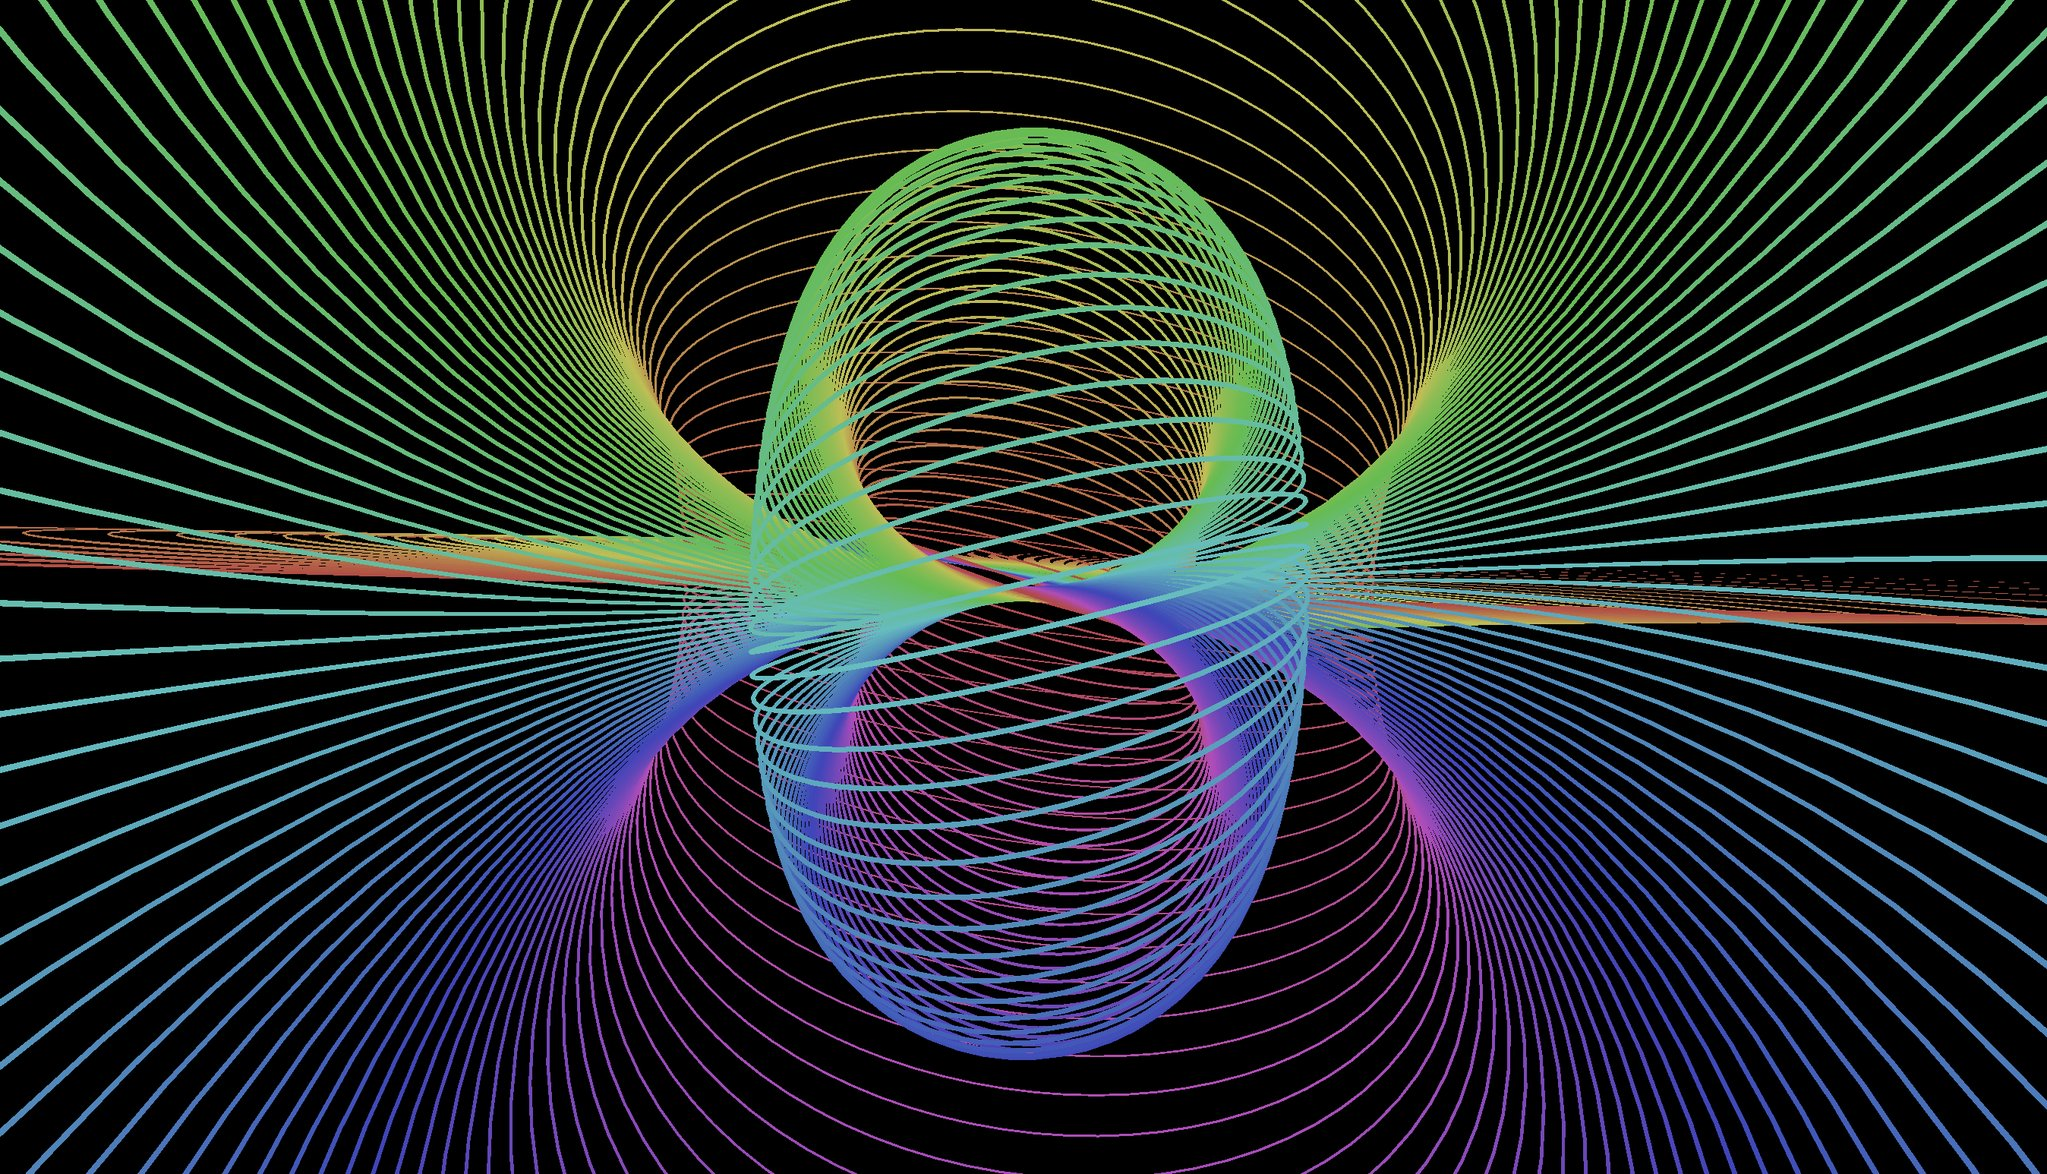
\includegraphics[scale=0.28]{hopf-2.jpeg}}
  \caption{Розшарування Хопфа}
\end{figure}

\begin{lstlisting}
var fiber = new THREE.Curve(),
    color = sphericalCoords.color;

fiber.getPoint = function(t) {
    var eta = sphericalCoords.eta,
        phi = sphericalCoords.phi,
        theta = 2 * Math.PI * t;
    var x1 = Math.cos(phi+theta) * Math.sin(eta/2),
        x2 = Math.sin(phi+theta) * Math.sin(eta/2),
        x3 = Math.cos(phi-theta) * Math.cos(eta/2),
        x4 = Math.sin(phi-theta) * Math.cos(eta/2);
    var m = mag([x1,x2,x3]),
        r = Math.sqrt((1-x4)/(1+x4));
        return new THREE.Vector3(r*x1/m,r*x2/m, r*x3/m);
    };
\end{lstlisting}

\newpage
\subsubsection*{Гомотопічна інтерпретація}

Can we reason about spheres without a metric? Yes!
But can we do this in a constructive way? Also yes.


\subsubsection{Розшарування Хопфа}

\begin{example} ($S^3$ Hopf Fiber).
Guillaume Brunerie.
\begin{lstlisting}
rot: (x : S1) -> Path S1 x x = split
    base -> loop1
    loop @ i -> constSquare S1 base loop1 @ i

mu : S1 -> equiv S1 S1 = split
    base -> idEquiv S1
    loop @ i -> equivPath S1 S1 (idEquiv S1)
                (idEquiv S1) (<j> \(x : S1) -> rot x @ j) @ i

H : S2 -> U = split
    north -> S1
    south -> S1
    merid x @ i -> ua S1 S1 (mu x) @ i

total : U = (c : S2) * H c
\end{lstlisting}
\end{example}

\begin{definition} (H-space).
H-space over a carrier $A$ is a tuple
$$
H_A=
\begin{cases}
A : U\\
e : A\\
\mu : A \rightarrow A \rightarrow A\\
\beta : (a:A) \rightarrow \Sigma (\mu(e,a)=a) (\mu(a,e)=a)
\end{cases}
$$.
\end{definition}

\begin{theorem} (Hopf Fibrations).
There are fiber bundles:\\
(S^0,S^1,p,S^1),
(S^1,S^3,p,S^2),
(S^3,S^7,p,S^4),
(S^7,S^{15},p,S^8).
\end{theorem}

\begin{definition} (Hopf Invariant).
Let $\phi: S^{2n-1} \rightarrow S^{n}$ a continuous map.
Then homotopy pushout (cofiber) of $\phi$ is
$cofib(\phi) = S^{n} \bigcup_\phi \mathbb{D}^{2n}$ has
ordinary cohomology
$$
H^{k}(cofib(\phi),\mathbb{Z})=
\begin{cases}
\mathbb{Z}\ for\ k=n,2n \\[2ex]
0\ otherwise
\end{cases}
$$
\end{definition}

Hence for $\alpha,\beta$ generators of the cohomology groups in
degree $n$ and $2n$, respectively, there exists an integer $h(\phi)$
that expresses the <b>cup product</b> square of $\alpha$
as a multiple of $\beta$ &mdash; $\alpha\sqcup\alpha=h(\phi)\cdot\beta$.
This integer $h(\phi)$ is called Hopf invariant of $\phi$.

\begin{theorem} (Adams, Atiyah).
Hopf Fibrations are only maps that have Hopf invariant $1$.
\end{theorem}



\subsection{Теорія (Ко)Гомологій}
\section{Диференціальна геометрія}
\subsection{V-многовиди}
\subsection{G-структури}
\subsection{H-простори}

\lstset{xleftmargin=-2.65cm}


\lstset{xleftmargin=0cm}

\include{apps}

\cite{Lof72}
\cite{Lof84}
\cite{Coq88}
\cite{Hofmann96}
\cite{Henk93}
\cite{Erik97}
\cite{Hermida95}
\cite{Curien08}
\cite{MacLane71}
\cite{Lawvere09}
\cite{Dybjer08}
\cite{Clairambault05}
\cite{Abel08}
\cite{Seely84}
\cite{Curien14}
\cite{Castellan14}
\cite{Voevodsky14}
\cite{Dybjer95}
\cite{Bishop67}
\cite{Nordstrom90}
\cite{Hermida98}
\cite{Barthe00}
\cite{Voevodsky15}
\cite{Sozeau}
\cite{Selsam16}
\cite{Bohm85}
\cite{Pfenning89}
\cite{Wadler90}
\cite{Gambino03}
\cite{Dybjer94}
\cite{Jacobs97}
\cite{Vene00}
\cite{Basold16}
\cite{Hofmann94}
\cite{Jacobs99}
\cite{Joyal14}
\cite{HoTT13}
\cite{Mortberg17}
\cite{Shulman15}
\cite{Orton17}
\cite{Huber16}
\cite{Huber17}
\cite{Angiuli16}
\cite{Angiuli162}

\bibliographystyle{ieeetr}
\bibliography{diss}

\end{document}
